\documentclass[../Thesis-IJspeert.tex]{subfiles}

\begin{document}

\graphicspath{ {"Dynamic Dipole Traps for Single Atoms/figs/"} }
\pgfplotsset{table/search path={"Dynamic Dipole Traps for Single Atoms/data/"}}

\chapter{Dynamic Dipole Traps for Single Atoms}
\addtocontents{toc}{\vskip-6pt\par\noindent\protect\textcolor{gray75}{\protect\rule{\textwidth}{0.5pt}}\par}
\label{chap:DynamicDipoleTrapsforSingleAtoms}

In this chapter, we investigate the effect of changing the depth of a static, optical dipole trap on the atom loading and loss rates and propose a feedback mechanism that enhances the trap filling ratio greatly beyond what is maximally achievable in the collisional blockade regime. Apart from requiring significantly less optical power with respect to the conventional approach of relocating atoms, this method reduces the need for atom rearrangement to achieve consistent filling of dipole trap arrays. 

\section{Introduction}

Single trapped atoms at temperatures near absolute zero constitute ideal information carriers in quantum computing and simulation. Recent advances in this field underpin the utility of using reconfigurable, optical tweezers to trap cold neutral atoms. This approach has enabled remarkable achievements in the context of quantum information science and many-body physics \cite{Labuhn2016, Endres2016, Bernien2017, Lienhard2018, Barredo2018}. Apart from being highly scalable \cite{Manetsch2024}, neutral atoms in reconfigurable microtraps exhibit long coherence times \cite{Norcia2019,Wu2019,Young2020} and allow for arbitrary qubit connectivity \cite{Beugnon2007,Bluvstein2022}. They furthermore enable fully programmable single-qubit rotations \cite{Ma2023} and are shown to yield a high readout and two-qubit gate fidelity \cite{Evered2023}. The combination of these characteristics fostered the development of a logical quantum processor based on reconfigurable atom arrays \cite{Bluvstein2023}. In the context of quantum repeaters and networks, arrays of individually controlled neutral atoms coupled to optical cavities are equally promising for generating efficient remote entanglement over a mesh of quantum nodes \cite{Wilk2007, rempe2012, Covey2023}. 

Single-atom optical dipole traps have been implemented using a large range of different techniques with varying degrees of configurability: acousto-optic deflectors \cite{Endres2016, Bernien2017}, micro-lens arrays \cite{OhldeMello2019}, standing wave dipole traps \cite{Alt2003, Gallego2018}, digital mirror devices (DMD) \cite{Stuart2018} and liquid crystal spatial light modulators (SLM) \cite{Bergamini2004, Kim2016}. The use of a DMD or liquid crystal SLM for holographic beam shaping extends the range of trapping geometries beyond periodic lattices to arbitrary configurations in up to three dimensions \cite{Barredo2018}.

With any of these trapping techniques, achieving consistent single-atom occupation across multiple trapping sites constitutes a challenging task, due to the fact that atoms enter the traps stochastically \cite{Grimm2000}. To be precise, in sufficiently tight dipole traps---those with a beam waist of around \SI{1}{\micro\meter}---single-atom loading is accomplished by virtue of light-assisted collisions, which cause a collisional blockade \cite{Schlosser2002}. This regime is characterised with a strong two-atom loss rate due to inelastic collisions, resulting in a negligible probability of finding a doubly occupied trap. When loading atoms directly from a magneto-optic trap (MOT) or optical molasses however, the time-averaged, single-atom occupation probability is limited to $0.5$. This implies that the likelihood of establishing fully occupied arrays of traps will decrease exponentially as the system size increases. The strategies to overcome this problem are to either increase the single-atom loading efficiency \cite{Fung2014} or to relocate ancillary atoms to vacant positions \cite{Vala2005}. Whilst this is typically accomplished with acousto-optic beam deflectors \cite{Barredo2018}, atom relocation has also been achieved through the use of dynamic holograms \cite{Kim2016,Kim2019}. When atoms are transported by means of dynamic holograms however, phase changes of a liquid crystal SLM or resettling oscillations of DMD micro-mirrors give rise to uncontrollable fluctuations in the trapping potential, causing a dramatic increase in the atom loss rate \cite{Stuart2018,McGloin2003}.

\section{The collisional blockade}
As aforementioned, the collisional blockade refers to a phenomenon that limits the number of atoms that can be trapped in a given region of space due to collisions between atoms. In this section, we discuss the relevant loading regimes by considering the dynamics of the number of trapped atoms, followed by a discussion of the light-assisted collisions that occur when the internuclear separation is sufficiently small.
\subsection{Atom number dynamics}
When a dipole trap with a small trapping volume is initially loaded from a low density MOT, the observed number of atoms $N$ in the trap is either zero or one, which corresponds to a statistical distribution of the atom number that is strongly sub-Poissonian. In order to understand the mechanism responsible for this phenomenon, let us consider the dynamics of the number of atoms in a trap that is subject to continuous atom loading at a rate $R$. Losses occur due to two main mechanisms: single-body losses caused by collisions with background gas atoms and two-body losses, due to inelastic collisions between the trapped atoms themselves. These processes occur at respective rates of $-\gamma_1 N$ and $-\gamma_2 N(N-1)$, in terms of the single-body ($\gamma_1$) and two-body ($\gamma_2$) decay coefficients, the latter of which being inversely proportional to the trap volume. The rate of change of $N$ is thus governed by the differential equation:
\begin{equation}
\frac{\mathrm{d}N}{\mathrm{d}t} = R - \gamma_1 N - \gamma_2 N (N-1)\,.
\end{equation}
In the steady state, two distinct parameter spaces can be identified \cite{Schlosser2002}: the weak and strong loading regimes. In the former regime, the loading rate $R$ (and therefore $\langle N \rangle$) is sufficiently small that the two-body loss term can be neglected, which results in the average number of atoms approaching the ratio $\langle N \rangle \rightarrow \sfrac{R}{\gamma} $. On the contrary, when $R$ (and therefore $\langle N \rangle$) is large, the two-body decay becomes the dominating loss channel, which leads to $\langle N \rangle \rightarrow \sqrt{ \sfrac{R}{\gamma_2} }$. The crossover between these two regimes is characterised by the critical atom number $ N_c = \sfrac{\gamma_1}{\gamma_2} $, which corresponds to a critical loading rate of $ R_c = \sfrac{\gamma_1^2}{\gamma_2} $. When the atom number exceeds $N_c$ (or when the loading rate exceeds $ R_c $), two-body collisions start to dominate the system dynamics. The collisional blockade occurs when the trapping volume and therefore the critical atom number is sufficiently small ($N_c \ll 1$) such that the two-body loss mechanism already dominates when a second atom enters the dipole trap.

\subsection{Light-assisted collisions}
Here, we discuss a semi-classical model that helps explain the dynamics of atom pairs during light-assisted, inelastic collisions, which are a key mechanism behind two-body loss in tightly confined dipole traps. Light-assisted collisions occur when two atoms interact in the presence of resonant light, facilitating transitions between electronic states. In a semi-classical model consisting of two \ce{^87Rb} atoms, this process involves excitation from the \ce{5\!^2S_{\sfrac{1}{2}}}\,+\,\ce{5\!^2S_{\sfrac{1}{2}}} ground state to the \ce{5\!^2S_{\sfrac{1}{2}}}\,+\,\ce{5\!^2P_{\sfrac{1}{2}}} excited state at a specific internuclear distance known as the Condon radius $R_C$ (see \autoref{lightassistedcollisions}).
\begin{figure}[h]
\centering
	\begin{tikzpicture}
	\pgfmathsetmacro{\eps}{4}
	\pgfmathsetmacro{\sig}{1.1}
	\pgfmathsetmacro{\min}{1}
	\pgfmathdeclarefunction{V}{1}{%
		\pgfmathparse{%
			4*\eps*((\sig/#1)^12-(\sig/#1)^6)
		}%
	}
	\begin{groupplot}[group style={group size=1 by 2,horizontal sep=0cm, vertical sep=0.cm},xmin=0,ymin=0,width=5.5cm,no markers]
	
	\nextgroupplot
	[
	xmin=17,
	xmax=38,
	ymin=-2,
	ytickmin=-1,
	axis y discontinuity=crunch,
	ymax=2,
	%xtick={1.4,1.6},
	xticklabels={},
	ylabel={Potential $U/h$ (\si{\giga\hertz})},
	height=5cm,
	axis x line*=top,
	ylabel style={xshift=-0.2cm}
	];
	
	
	\node[] (source) at (axis cs:1.6, 2.7){};
	\node (destination) at (axis cs:1.6, 6.7){};
	\draw[->, color=markrood](source)--(destination);
	
	\node[] (source) at (axis cs:1.4, 5.3){};
	\node (destination) at (axis cs:1.4, 2.55){};
	\draw[->, color=markrood,decorate,decoration={snake,amplitude=.4mm,segment length=1.5mm}](source)--(destination);
	
	\draw[color=markgrijs, dashed] 
	(axis cs:27.65, 0.4) -- (axis cs:27.65, 2);
	\draw[color=markgrijs, dashed] 
	(axis cs:22.5, -0.525) -- (axis cs:22.5, 2);
	
	\draw[color=markgrijs, dashed] 
	(axis cs:15, 0) -- (axis cs:40, 0);
	\draw[color=markrood, dashed] 
	(axis cs:21, -0.3) -- (axis cs:27.2, -0.3);
	\draw[color=markdiepblauw, dashed] 
	(axis cs:21, 0.3) -- (axis cs:27.5, 0.3);
	

	
	\pgfplotsset{
		after end axis/.append code={
			\node [align=center] at (axis cs:27.65,2.3) {\footnotesize $R_C$};
			\node [align=center] at (axis cs:22.5,2.3) {\footnotesize $R_S$};
		}
	}
	
	\draw[->, markdiepblauw] (axis cs:27.8,-4) to (axis cs:27.8, 0.31);
	\draw[->, color=markdiepblauw,decorate,decoration={snake,amplitude=.4mm,segment length=1.497mm}](axis cs:30,0.245)--(axis cs:30,-4);
	
	\addplot[markrood] table [col sep=comma] {redline.csv};
	\addplot[markdiepblauw] table [col sep=comma] {blueline.csv};
	
	\draw[->, markrood] (axis cs:27.5,-4) to (axis cs:27.5, -0.31);
	\draw[->, color=markrood,decorate,decoration={snake,amplitude=.4mm,segment length=1.483mm}](axis cs:22.5,-0.525)--(axis cs:22.5,-4);
	
	
	\draw[->, black] (axis cs:35.5,-2) -- node[left] {\footnotesize $\nu_0$} (axis cs:35.5, 0);
	\draw[<->, markrood] (axis cs:21,-0.3) to (axis cs:21, 0.0);
	%\draw[->, markrood] (axis cs:19,-0.5) to (axis cs:19, -0.3);
	
	\draw[<->, markdiepblauw] (axis cs:21,0.3) to (axis cs:21, 0);
	%\draw[->, markblauw] (axis cs:22,-0.2) to (axis cs:22, 0);
	
	\node[align=left, color=markdiepblauw] at (axis cs:19,0.2) {\footnotesize $\delta$};
	\node[align=left, color=markrood] at (axis cs:19,-0.2) {\footnotesize $\delta$};
	\node[rotate=191,color=markrood] at (axis cs:25,-0.43) {\footnotesize$\rightharpoonup$};
	
	\node[rotate=-15,color=markdiepblauw] at (axis cs:25,0.48) {\footnotesize$\leftharpoonup$};
	
	\node[rotate=-9,color=markdiepblauw] at (axis cs:29,0.305) {\footnotesize$\rightharpoonup$};
	\node[color=markdiepblauw] at (axis cs:31,-0.5) {\footnotesize$4$};
	\node[color=markdiepblauw] at (axis cs:28.7,0.55) {\footnotesize$3$};
	\node[color=markdiepblauw] at (axis cs:25.5,0.7) {\footnotesize$2$};
	\node[color=markdiepblauw] at (axis cs:28.5,-1.7) {\footnotesize$1$};
	\node[color=markrood] at (axis cs:26.8,-1.7) {\footnotesize$1$};
	\node[color=markrood] at (axis cs:25.2,-0.7) {\footnotesize$2$};
	\node[color=markrood] at (axis cs:21.5,-1) {\footnotesize$3$};
	
	\pgfplotsset{
		after end axis/.append code={
			\node [anchor=east,text width=2cm,align=left] at (axis cs:50.5,-2.13) {\footnotesize \ce{5\!^2S_{\sfrac{1}{2}}}\,+\,\ce{5\!^2S_{\sfrac{1}{2}}}};
			\node [anchor=east,text width=2cm,align=left] at (axis cs:50.5,0) {\footnotesize \ce{5\!^2S_{\sfrac{1}{2}}}\,+\,\ce{5\!^2P_{\sfrac{1}{2}}}};
			\node [draw,fill=white,anchor=east,align=center] at (axis cs:37,1.45) {\footnotesize $F=F'=2$};
		}
	}
	
	
	
	\nextgroupplot
	[
	xmin=17,
	xmax=38,
	ymin=-3.8,
	ymax=-3,
	xlabel={Internuclear separation $R$ (\si{\nano\meter})},
	ytick={},
	yticklabels={,},
	ytick style={draw=none},
	axis x line*=bottom,
	height=2cm
	];
	\addplot[black] table [x expr={\thisrowno{0}}, 
	y expr={\thisrowno{1}}, col sep=comma] {blackline.csv};
	
	\draw[->, black] (axis cs:35.5,-2.5) to (axis cs:35.5, -3.25);
	\draw[-, markrood] (axis cs:27.5,-2.5) to (axis cs:27.5, -3.25);
	\draw[-, markdiepblauw] (axis cs:27.8,-2.5) to (axis cs:27.8, -3.25);
	
	\draw[->, color=markrood,decorate,decoration={snake,amplitude=.4mm,segment length=1.49mm}](axis cs:22.5,-2)--(axis cs:22.5,-3.315);
	
	\draw[->, color=markdiepblauw,decorate,decoration={snake,amplitude=.4mm,segment length=1.483mm}](axis cs:30,-0.51)--(axis cs:30,-3.23);
	
	\end{groupplot}
	\end{tikzpicture}
\caption[Molecular interaction potentials and light-assisted collision processes for two \ce{^87Rb} atoms]{An example of attractive (red) and repulsive (blue) molecular interaction potentials on the $\mathrm{D}1$ line of two \ce{^87Rb} atoms as a function of the internuclear separation $R$. Light-assisted collision processes are shown for red- and blue-shifted light fields, both detuned by $\delta=\sfrac{\Delta}{2\pi}$ from the free-space transition frequency $\nu_0=\sfrac{\omega_0}{2\pi}$. For red-detuned light, this process involves the excitation (1) from \ce{5\!^2S_{\sfrac{1}{2}}}\,+\,\ce{5\!^2S_{\sfrac{1}{2}}} to \ce{5\!^2S_{\sfrac{1}{2}}}\,+\,\ce{5\!^2P_{\sfrac{1}{2}}} at an internuclear distance of $R_C$. This is followed by an acceleration (2) through the attractive potential until spontaneous emission to the ground state (3) occurs at $R_S$. For blue-detuned light, the potential is repulsive, which means that the atoms are slowed down (2) before moving away from each other (3) until spontaneous emission occurs (4). Data adapted from \cite{Pampel_2024}.}
\label{lightassistedcollisions} 
\end{figure}
The excited state is influenced by long-range resonant dipole interactions, leading to attractive or repulsive potentials that scale with $\sfrac{1}{R^3}$. In general, fine and hyperfine interactions contribute to the complexity of these interaction potentials. When two atoms reach an internuclear separation of $R_C$, the laser light becomes resonant with the excited-state potential, coupling the ground and excited states. For red-detuned light, atoms transition to the attractive potential, accelerating towards each other. Upon spontaneous decay back to the ground state, the atom pair gains kinetic energy from the difference in potential energy between the points $R_C$ and $R_S$, the latter being defined as the internuclear separation at which the spontaneous emission occurred. This energy gain can lead to atoms being ejected from the trap if the final kinetic energy exceeds the trap depth. 

\section{Experimental apparatus}
Among the various techniques for dipole trapping, holographic beam shaping offers an outstanding degree of configurability. It allows for independent control over individual trapping sites, which is essential for a scalable design. In this section, we discuss the experimental setup for trapping arrays of \ce{^87Rb} atoms with holographic optical tweezers.

\subsection{Overview}
An overview of the experimental setup is shown in \autoref{overviewsetup}.
\begin{figure}[t]
	\centering
	\begin{tikzpicture}
	\node[anchor=south west,inner sep=0] (image) at (0,0) {\includegraphics[width=1.0\textwidth]{{"assembly"}.png}};
	\begin{scope}[x={(image.south east)},y={(image.north west)}]
	
	%\node[] at (0.052,0.65) {\small\textcolor{markgrijs}{\SI{1064}{\nano\meter}}};
	\end{scope}
	
	\end{tikzpicture}
	\caption[Optical setup for the generation of dipole traps and a MOT]{(Left) Optical setup for the generation of \SI{1064}{\nano\meter} dipole traps and the detection of fluorescence. A spatial light modulator (SLM) generates a tweezer array inside the glass cell, monitored via a CCD. A dichroic mirror (DM) redirects the fluorescence into a detection path, where atoms are imaged using an EMCCD camera. Numbers indicate the beam magnification factors. (Right) Optical setup for the generation of the MOT inside a glass cell using $3$ retro-reflected beams. To achieve collimation and circular polarisation of the beams, we employ $f=\SI{30}{\milli\meter}$ lenses and pairs of quarter-wave plates, respectively. A pair of high-NA lenses focus and image the dipole trapping light.}
	\label{overviewsetup} 
\end{figure}
In this setup, \ce{^{87}Rb} atoms are cooled in a MOT on the $\mathrm{D}2$ transition ($\ce{5\!^2S_{\sfrac{1}{2}}} \, \leftrightarrow \, \ce{5\!^2P_{\sfrac{3}{2}}}$ at \SI{780.246}{\nm}) and eventually loaded into optical dipole-force traps established at a wavelength of \SI{1064}{\nm}. The MOT is formed using $3$ retro-reflected, circularly polarised beams, each consisting of overlapping cooling and repump beams with a $\sfrac{1}{e^2}$ beam diameter of \SI{5}{\milli\meter} and optical powers of \SI{1.5}{\milli\watt} and \SI{0.5}{\milli\watt}, respectively. The two diagonal beams are oriented at angles of \ang{30} with respect to the horizontal axis. Depending on the experiment, the cooling light is red-detuned from the $F=2 \, \leftrightarrow \, F'=3$ transition by either a fixed or time-varying frequency. Any population that decays into the $\ket{F=1}$ ground state is repumped to $\ket{F=2}$ with light resonant to the $\ket{F=1}\leftrightarrow\ket{F'=2}$ transition. The MOT is positioned within a cuboid glass cell vacuum chamber (ColdQuanta) that is kept under ultra-high vacuum ($\sim\!\SI{1e-10}{\milli\bar}$). The cell walls are equipped with an anti reflective coating that is specified for both \SI{780}{\nm} and \SI{1064}{\nm} (\SI{< 0.2}{\percent} for $\SI{650}{\nm} \leq \lambda \leq \SI{1100}{\nm}$ and angle of incidence between \SI{\pm 10}{\degree}, \SI{< 0.5}{\percent} for $\SI{760}{\nm} \leq \lambda \leq \SI{860}{\nm}$ and angle of incidence between \SI{\pm 45}{\degree}). The magnetic field is generated using a pair of anti-Helmholtz coils which are oriented along the long axis of the glass cell and establish a field gradient of \SI{13}{\gauss\per\centi\meter} at the quadrupole centre. The laser that generates the dipole traps is a continuous-wave fibre laser (Quantel EYLSA), which outputs single mode, narrow linewidth (\SI{<700}{\kHz}) light at \SI{1064}{\nm}, featuring an $M^2$ beam quality factor of \num{1.6}. Through the use of a telescope, the trapping light is first sent through an acousto-optic modulator (AOM), which allows for fast modulation of the overall trapping power. Following a subsequent expansion of the beam, a computer-generated phase pattern is imposed via a $512\times512$ pixel liquid crystal SLM (Meadowlark ODPDM512-1064), positioned in a Fourier plane of the light path. This can be viewed as an artificial hologram that gives rise to an intensity pattern in the image plane. This pattern, which contains all dipole traps, can be identified as the Fourier transformed light field that passes the SLM. By using an iterative approach based on feedback from the measured intensity of the generated trapping sites in combination with the mixed-region amplitude freedom (MRAF) algorithm \cite{Pasienski2008} to generate arbitrary phase patterns, we construct a uniform tweezer grid in the focal plane with $\sfrac{1}{e^2}$ trap diameters of \SI{2.2}{\micro\meter}, allowing for parallel data acquisition from multiple traps. A pair of achromatic, compound lens systems ($\mathrm{NA} = 0.6$) focus and recollimate the trapping light after a second beam expansion, such that traps can be monitored using a CCD camera (Daheng Imaging MER-132-30UM/C). The numerical aperture of \num{0.6} equates to a \SI{10}{\percent} collection efficiency of the fluorescence light, which is directed towards an EMCCD camera (Princeton Instruments ProEM-HS: 512BX3) via a dichroic mirror (Thorlabs DMLP950L) with a cut-off wavelength of \SI{950}{\nm} to block any trapping light from reaching the camera. In addition, a \SI{780}{\nm} bandpass filter (Semrok \num{780}/\SI{12}{\nm} BrightLine single-band) is placed directly in front of the EMCCD camera and eliminates any remaining light at \SI{1064}{\nm}.
\iffalse
\begin{figure}[h]
	\centering
	\begin{tikzpicture}
	\node[anchor=south west,inner sep=0] (image) at (0,0) {\includegraphics[width=0.9\textwidth]{{"setup"}.pdf}};
	\begin{scope}[x={(image.south east)},y={(image.north west)}]
	
	%\draw[help lines,xstep=.1,ystep=.1] (0,0) grid (1,1);
	%\foreach \x in {0,1,...,9} { \node [anchor=north] at (\x/10,0) {0.\x}; }
	%\foreach \y in {0,1,...,9} { \node [anchor=east] at (0,\y/10) {0.\y}; }
	
	\node[] at (0.052,0.65) {\small\textcolor{markgrijs}{\SI{1064}{\nano\meter}}};
	\node[] at (0.13,0.95) {\small\textcolor{markgrijs}{$\sfrac{\lambda}{2}$}};
	\node[] at (0.35,0.95) {\small\textcolor{markgrijs}{$\sfrac{\lambda}{2}$}};
	\node[] at (0.41,0.65) {\small\textcolor{markgrijs}{AOM}};
	\node[] at (0.6,0.78) {\small\textcolor{markgrijs}{$\sfrac{\lambda}{2}$}};
	\node[] at (0.73,0.66) {\small\textcolor{markgrijs}{$\sfrac{\lambda}{2}$}};
	\node[] at (0.95,0.07) {\small\textcolor{markgrijs}{SLM}};
	\node[] at (0.47,0.4) {\small\textcolor{markrood}{MOT}};
	\node[] at (0.29,0.225) {\small\textcolor{markrood}{CCD}};
	\node[] at (0.7,0.225) {\small\textcolor{markgrijs}{DM}};
	\node[] at (0.55,0.05) {\small\textcolor{markrood}{EMCCD}};
	\node[] at (0.28,0.6) {\small\textcolor{markblauw}{$\times 0.075$}};
	\node[] at (0.485,0.53) {\small\textcolor{markblauw}{$\times 3.3$}};
	\node[] at (0.77,0.07) {\small\textcolor{markblauw}{$\times 4.8$}};
	\end{scope}
	
	\end{tikzpicture}
	\caption[An example of a floating figure]{Schematic overview of the experimental setup. The vacuum chamber and the optics required to generate the MOT are not shown.} % The text in the square bracket is the caption for the list of figures while the text in the curly brackets is the figure caption
	\label{setup} 
\end{figure}
\fi

\subsection{Laser frequency stabilisation}
The lasers that generate the cooling and repumping light for the MOT in this setup are both Toptica DL100 external cavity diode lasers (ECDL), the frequencies of which are locked using a configuration as shown in \autoref{lockingsetup}. The frequency of the cooling ECDL is stabilised by means of modulation transfer spectroscopy (MTS), which, as detailed in \cite{McCarron2008}, produces dispersive-like lineshapes with a flat, zero background. This results in the zero-crossings of the modulation transfer signal being precisely centred on atomic transitions. In contrast to saturation spectroscopy, the signal in MTS arises mainly from closed atomic transitions---those in which atoms return to the same ground state after excitation rather than decaying to different states.
\begin{figure}[t]
	\newcommand\xmin{0.64}
	\newcommand\xmax{0.83}
	\newcommand\ymin{0.045}
	\newcommand\ymax{0.95}
	\centering
	\begin{tikzpicture}
	\node[anchor=south west,inner sep=0] (image) at (0,0)
	{\includegraphics[width=1.0\textwidth]{{"coolingrepump"}.pdf}};
	\begin{scope}[x={(image.south east)},y={(image.north west)}]
	
	%\draw[help lines,xstep=.1,ystep=.1] (0,0) grid (1,1);
	%\foreach \x in {0,1,...,9} { \node [anchor=north] at (\x/10,0) {0.\x}; }
	%\foreach \y in {0,1,...,9} { \node [anchor=east] at (0,\y/10) {0.\y}; }
	
	\node[anchor=mid west] at (0.0,0.805) {\footnotesize\textcolor{markrood}{\!Repump ECDL}};
	\node[anchor=west] at (0.0,0.555) {\footnotesize\textcolor{markrood}{\!Cooling ECDL}};
	
	\node[anchor=mid west] at (\xmin,\ymax) {\footnotesize\textcolor{black}{phase shifter}};
	
	\node[anchor=mid west] at (\xmin,{\ymin+6*(\ymax-\ymin)/7}) {\footnotesize\textcolor{black}{mixer}};
	
	\node[anchor=mid west] at (\xmin,{\ymin+5*(\ymax-\ymin)/7}) {\footnotesize\textcolor{black}{EOM}};
	
	\node[anchor=mid west] at (\xmin,{\ymin+4*(\ymax-\ymin)/7}) {\footnotesize\textcolor{black}{isolator}};
	
	\node[anchor=mid west] at (\xmin,{\ymin+3*(\ymax-\ymin)/7}) {\footnotesize\textcolor{black}{AOM}};
	
	\node[anchor=mid west] at (\xmin,{\ymin+2*(\ymax-\ymin)/7}) {\footnotesize\textcolor{black}{photodiode}};
	
	\node[anchor=mid west] at (\xmin,{\ymin+1*(\ymax-\ymin)/7}) {\footnotesize\textcolor{black}{vapour cell}};
	
	\node[anchor=mid west] at (\xmin,\ymin) {\footnotesize\textcolor{black}{fibre coupler}};
	
	
	\node[anchor=mid west] at (\xmax,\ymax) {\footnotesize\textcolor{black}{iris}};
	
	\node[anchor=mid west] at (\xmax,{\ymin+6*(\ymax-\ymin)/7}) {\footnotesize\textcolor{black}{$\sfrac{\lambda}{4}$ waveplate}};
	
	\node[anchor=mid west] at (\xmax,{\ymin+5*(\ymax-\ymin)/7}) {\footnotesize\textcolor{black}{$\sfrac{\lambda}{2}$ waveplate}};
	
	\node[anchor=mid west] at (\xmax,{\ymin+4*(\ymax-\ymin)/7}) {\footnotesize\textcolor{black}{lens}};
	
	\node[anchor=mid west] at (\xmax,{\ymin+3*(\ymax-\ymin)/7}) {\footnotesize\textcolor{black}{beam block}};
	
	\node[anchor=mid west] at (\xmax,{\ymin+2*(\ymax-\ymin)/7}) {\footnotesize\textcolor{black}{PBS}};
	
	\node[anchor=mid west] at (\xmax,{\ymin+1*(\ymax-\ymin)/7}) {\footnotesize\textcolor{black}{low-pass filter}};
	
	\node[anchor=mid west] at (\xmax,\ymin) {\footnotesize\textcolor{black}{PID lock}};
	
	
	
	\node[anchor=west] at (0.328,0.804) {\sc\footnotesize\textcolor{black}{a}};
	
	\node[anchor=west] at (0.532,0.053) {\sc\footnotesize\textcolor{black}{b}};
	
	\node[anchor=west] at (0.228,0.555) {\sc\footnotesize\textcolor{black}{c}};
	
	\node[anchor=west] at (0.173,0.095) {\sc\footnotesize\textcolor{black}{d}};
	
	\node[anchor=west] at (0.199,0.235) {\tiny\textcolor{markrood}{\rotatebox[origin=c]{90}{probe}}};
	
	\node[anchor=west] at (0.257,0.235) {\tiny\textcolor{markrood}{\rotatebox[origin=c]{90}{pump}}};
	
	
	\end{scope}
	
	\end{tikzpicture}
	\caption[Electro-optical setup for the frequency stabilisation of the cooling and repumping light]{Electro-optic setup for the frequency stabilisation of the cooling and repumping light required for the generation of the MOT as shown in \autoref{overviewsetup}. The lenses in this diagram all have focal lengths of \SI{150}{\milli\meter}. The fibre outputs at \textsc{b} and \textsc{c} lead directly to the MOT, whereas the outputs at \textsc{c} and \textsc{d} are combined on a photodiode to extract the beat note used in a frequency offset lock (not shown) for the repump ECDL. All fibres are polarisation maintaining.}
	\label{lockingsetup} 
\end{figure}
This feature makes MTS particularly useful for isolating specific transitions in atomic spectra, especially when the spectrum includes several closely spaced transitions. For the implementation of MTS, a fraction of the cooling light is split using a half-wave plate and a polarising beam splitter (PBS) before it is frequency shifted by \SI{-206}{\mega\hertz} in a double-pass AOM configuration. Thereafter, the beam is divided into \SI{0.5}{\milli\watt} pump and probe beams, the former being phase-modulated with an electro-optic modulator (EOM) at a modulation frequency of $\omega_m=\SI{25}{\mega\hertz}$. The resulting light can be represented in terms of the carrier frequency $\omega_c$ and modulation index $\delta$ as $E(t)=E_0\sin(\omega_c t+\delta\sin(\omega_m t))$. The pump and probe beams propagate in opposite directions and are aligned to run collinearly through a \SI{5}{\centi\meter} long \ce{Rb} vapour cell at room temperature. A four-wave mixing process in the vapour cell involves the combination of the two frequency components of the pump beam with the probe beam as a result of the non-linearity of the absorption medium. The result is a fourth wave for each sideband of the pump beam that appears as a sideband on the probe beam. A photodetector extracts the corresponding beat signal $S_b$, which, for $\delta < 1$, can be approximated as \cite{Shirley1982}
\begin{align}
\label{mtsbeatsignal}
\begin{split}
	S_b(\omega_m) \propto \frac{J_0(\delta)J_1(\delta)}{\sqrt{\Gamma^2+\omega_m^2}}  \Big[ (L_{-1} - L_{-\sfrac{1}{2}} + L_{\sfrac{1}{2}} - L_1) &\cos(\omega_m t + \phi) \\
	+ (D_{1} - D_{\sfrac{1}{2}} - D_{-\sfrac{1}{2}} + D_{-1}) &\sin(\omega_m t + \phi) \Big]\,,
\end{split}
\end{align}
written in terms of the natural linewidth $\Gamma$ of the transition and the phase $\phi$ of the detector signal with respect to the modulation field $E(t)$. $J_n(\delta)$ represents the $n^{\text{th}}$ order Bessel function, while $L_n$ and $D_n$ represent the absorptive and dispersive components, which can be written as
\begin{align}
L_n = \frac{\Gamma^2}{\Gamma^2 + (\Delta - n \omega_m)^2}\quad\quad D_n = \frac{\Gamma (\Delta - n \omega_m)}{\Gamma^2 + (\Delta - n \omega_m)^2}\,,
\end{align}
in terms of the laser frequency detuning $\Delta$ from the line centre. We demodulate the signal $S_b$ through the use of a mixer and low-pass filter as shown in \autoref{lockingsetup}. By tuning the phase $\phi$, one can select either the in-phase component ($\phi=0$) or the quadrature component ($\phi=\sfrac{\pi}{2}$) in \autoref{mtsbeatsignal}. Either component is an odd function of $\Delta$ and provided that $\omega_m\le \Gamma$, features a large gradient at resonance, yielding a suitable error signal that feeds into a PID controller (Toptica PID100) that locks the frequency of the branched beam to the $ F = 2 \leftrightarrow F' = 3 $ cooling transition. In a secondary, double-pass AOM configuration, the frequency of the unbranched beam is shifted by \SI{-220}{\mega\hertz} to establish three red-detuned cooling beams for the MOT. To stabilise the frequency of the repump ECDL, we employ a frequency offset lock \cite{Schnemann1999} operating at \SI{6.5}{\giga\hertz}, such that the repumping light is resonant to the $ F = 1 \leftrightarrow F' = 2 $ transition after the ECDL output beam has passed through an AOM that shifts its frequency by \SI{+107}{\mega\hertz}. The beat note is locked to a reference oscillator using an offset phase lock servo (Vescent D2-135). All optical components shown in \autoref{lockingsetup} are mounted on an optical breadboard with Sorbothane feet to establish vibrational isolation from the optical table, which significantly enhances the long term stability of the frequency locks.

\subsection{Magnetic fields}
The magnetic field for the MOT is produced by a pair of anti-Helmholtz
coils consisting of N = 159 turns of 18 AWG copper wire, with a radius
of R = 4 cm and a separation of 8 cm. By equation (2.22), operating the
coils at a current of 2.0 A gives a magnetic field gradient of 13 Gauss cm−1
at the quadrupole centre. The three compensation coils each have N = 9
turns of 18 AWG copper wire on a square frame. The main MOT coils and
the compensation coils are all mounted to a set of four vertical rails, with
the main MOT coils positioned such that the glass cell goes through their
centre.
Operating the MOT coils at 2.0 A for a long period of time (several hours)
causes the temperature to rise up to a maximum of approximately 50 ◦C. This
temperature is not hot enough to require the use of any cooling mechanisms.
When operating the experiment, the MOT coils should be switched on for
approximately half an hour before beginning work, so that the temperature
is starting to stabilise, since significant changes in temperature can affect the
alignment and optimal values of other parameters.

\section{Static arrays of dipole traps}
Prior to performing more advanced experiments such as moving atoms using dynamic holograms, it is essential to probe and understand the behaviour of atoms captured with static holographic tweezers. In this section, we present our analysis of the trapping potential as well as the collisional blockade, ac-stark effect, lifetime and filling fraction of traps with varying depths in a static trapping potential landscape.





%------------------------------------------------

%----------------------------------------------------------------------------------------
%	RESULTS AND DISCUSSION
%----------------------------------------------------------------------------------------


\subsection{Atom fluorescence and ac-Stark effect}
\label{stark}
In order to parallelise the trap analysis, we calculate the kinoform for a $6\times6$ grid of trapping sites with varying potential depths.\footnote{In this report, we have only considered a grid with varying traps for which individual and precise depth adjustment is unnecessary. However, calculating the kinoform for a grid containing identical traps requires a more careful approach. In a first attempt to generate uniform holographic microtrap arrays, we have observed inconsistent lifetimes and filling fractions. The origin of this problem is that aberrations induced by the optics alter the shape and depth of the microtraps. It has been shown that this effect can be mitigated by using the SLM for aberration correction \cite{imr2010,Kim2019} and by using iterative feedback loops that correct each microtrap based on measurements of both the trapping and fluorescence light \cite{Tamura2016}.} The recorded intensity profile is shown in \autoref{36a}.
\begin{figure}[t]
	\vspace{0em}
	\centering
	\begin{subfigure}[b]{.32\linewidth}
		\begin{tikzpicture}
		\centering
		\node[inner sep=0] (image) {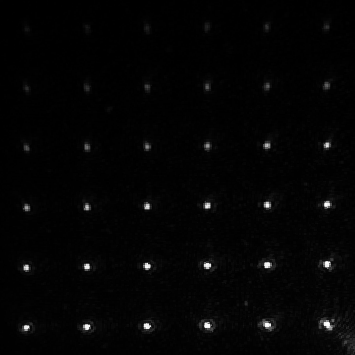
\includegraphics[width=1.4in] {grid0.pdf}};;
		\draw[white, fill=white] (0.95,1.4) rectangle (1.45,1.45);
		\node[color=white] at (1.03,1.1) {\footnotesize \SI{20}{\micro\meter}};
		\end{tikzpicture}
		\centering
		\caption{}
		\label{36a}
	\end{subfigure}
	\begin{subfigure}[b]{.32\linewidth}
		\begin{tikzpicture}
		\centering
		\node[inner sep=0] (image) {
\includegraphics[width=1.4in] {grid6x61blue.pdf}};;
		
		\node[anchor=south , color=white] at (-42.5pt,-50.5pt) {\scriptsize $25$};
		\node[anchor=south , color=white] at (-42.5pt,-33.6pt) {\scriptsize $19$};
		\node[anchor=south , color=white] at (-42.5pt,-16.7pt) {\scriptsize $12$};
		\node[anchor=south , color=white] at (-42.5pt,0.5pt) {\scriptsize $6.5$};
		\node[anchor=south , color=white] at (-42.5pt,17.1pt) {\scriptsize $3.4$};
		\node[anchor=south , color=white] at (-42.5pt,34pt) {\scriptsize $1.4$};
		
		\node[anchor=south , color=white] at (-25.6pt,-50.5pt) {\scriptsize $31$};
		\node[anchor=south , color=white] at (-25.6pt,-33.6pt) {\scriptsize $24$};
		\node[anchor=south , color=white] at (-25.6pt,-16.7pt) {\scriptsize $15$};
		\node[anchor=south , color=white] at (-25.6pt,0.5pt) {\scriptsize $9.3$};
		\node[anchor=south , color=white] at (-25.6pt,17.1pt) {\scriptsize $1.5$};
		\node[anchor=south , color=white] at (-25.6pt,34pt) {\scriptsize $1.6$};
		
		\node[anchor=south , color=white] at (-8.7pt,-50.5pt) {\scriptsize $37$};
		\node[anchor=south , color=white] at (-8.7pt,-33.6pt) {\scriptsize $30$};
		\node[anchor=south , color=white] at (-8.7pt,-16.7pt) {\scriptsize $20$};
		\node[anchor=south , color=white] at (-8.7pt,0.5pt) {\scriptsize $10$};
		\node[anchor=south , color=white] at (-8.7pt,17.1pt) {\scriptsize $5.3$};
		\node[anchor=south , color=white] at (-8.7pt,34pt) {\scriptsize $2.5$};
		
		\node[anchor=south , color=white] at (8.2pt,-50.5pt) {\scriptsize $42$};
		\node[anchor=south , color=white] at (8.2pt,-33.6pt) {\scriptsize $34$};
		\node[anchor=south , color=white] at (8.2pt,-16.7pt) {\scriptsize $23$};
		\node[anchor=south , color=white] at (8.2pt,0.5pt) {\scriptsize $12$};
		\node[anchor=south , color=white] at (8.2pt,17.1pt) {\scriptsize $6.8$};
		\node[anchor=south , color=white] at (8.2pt,34pt) {\scriptsize $2.8$};
			
		\node[anchor=south , color=white] at (25.1pt,-50.5pt) {\scriptsize $46$};
		\node[anchor=south , color=white] at (25.1pt,-33.6pt) {\scriptsize $36$};
		\node[anchor=south , color=white] at (25.1pt,-16.7pt) {\scriptsize $24$};
		\node[anchor=south , color=white] at (25.1pt,0.5pt) {\scriptsize $15$};
		\node[anchor=south , color=white] at (25.1pt,17.1pt) {\scriptsize $6.5$};
		\node[anchor=south , color=white] at (25.1pt,34pt) {\scriptsize $3.4$};
		
		\node[anchor=south , color=white] at (42pt, -50.5pt) {\scriptsize $51$};
		\node[anchor=south , color=white] at (42pt, -33.6pt) {\scriptsize $41$};
		\node[anchor=south , color=white] at (42pt, -16.7pt) {\scriptsize $29$};
		\node[anchor=south , color=white] at (42pt, 0.5pt) {\scriptsize $17$};
		\node[anchor=south , color=white] at (42pt, 17.1pt) {\scriptsize $7.9$};
		\node[anchor=south , color=white] at (42pt, 34pt) {\scriptsize $3.6$};
		
		\end{tikzpicture}
		\centering
		\caption{}
		\label{36b}
	\end{subfigure}
	\begin{subfigure}[b]{.32\linewidth}
		\begin{tikzpicture}
		\centering
		\node[inner sep=0] (image) {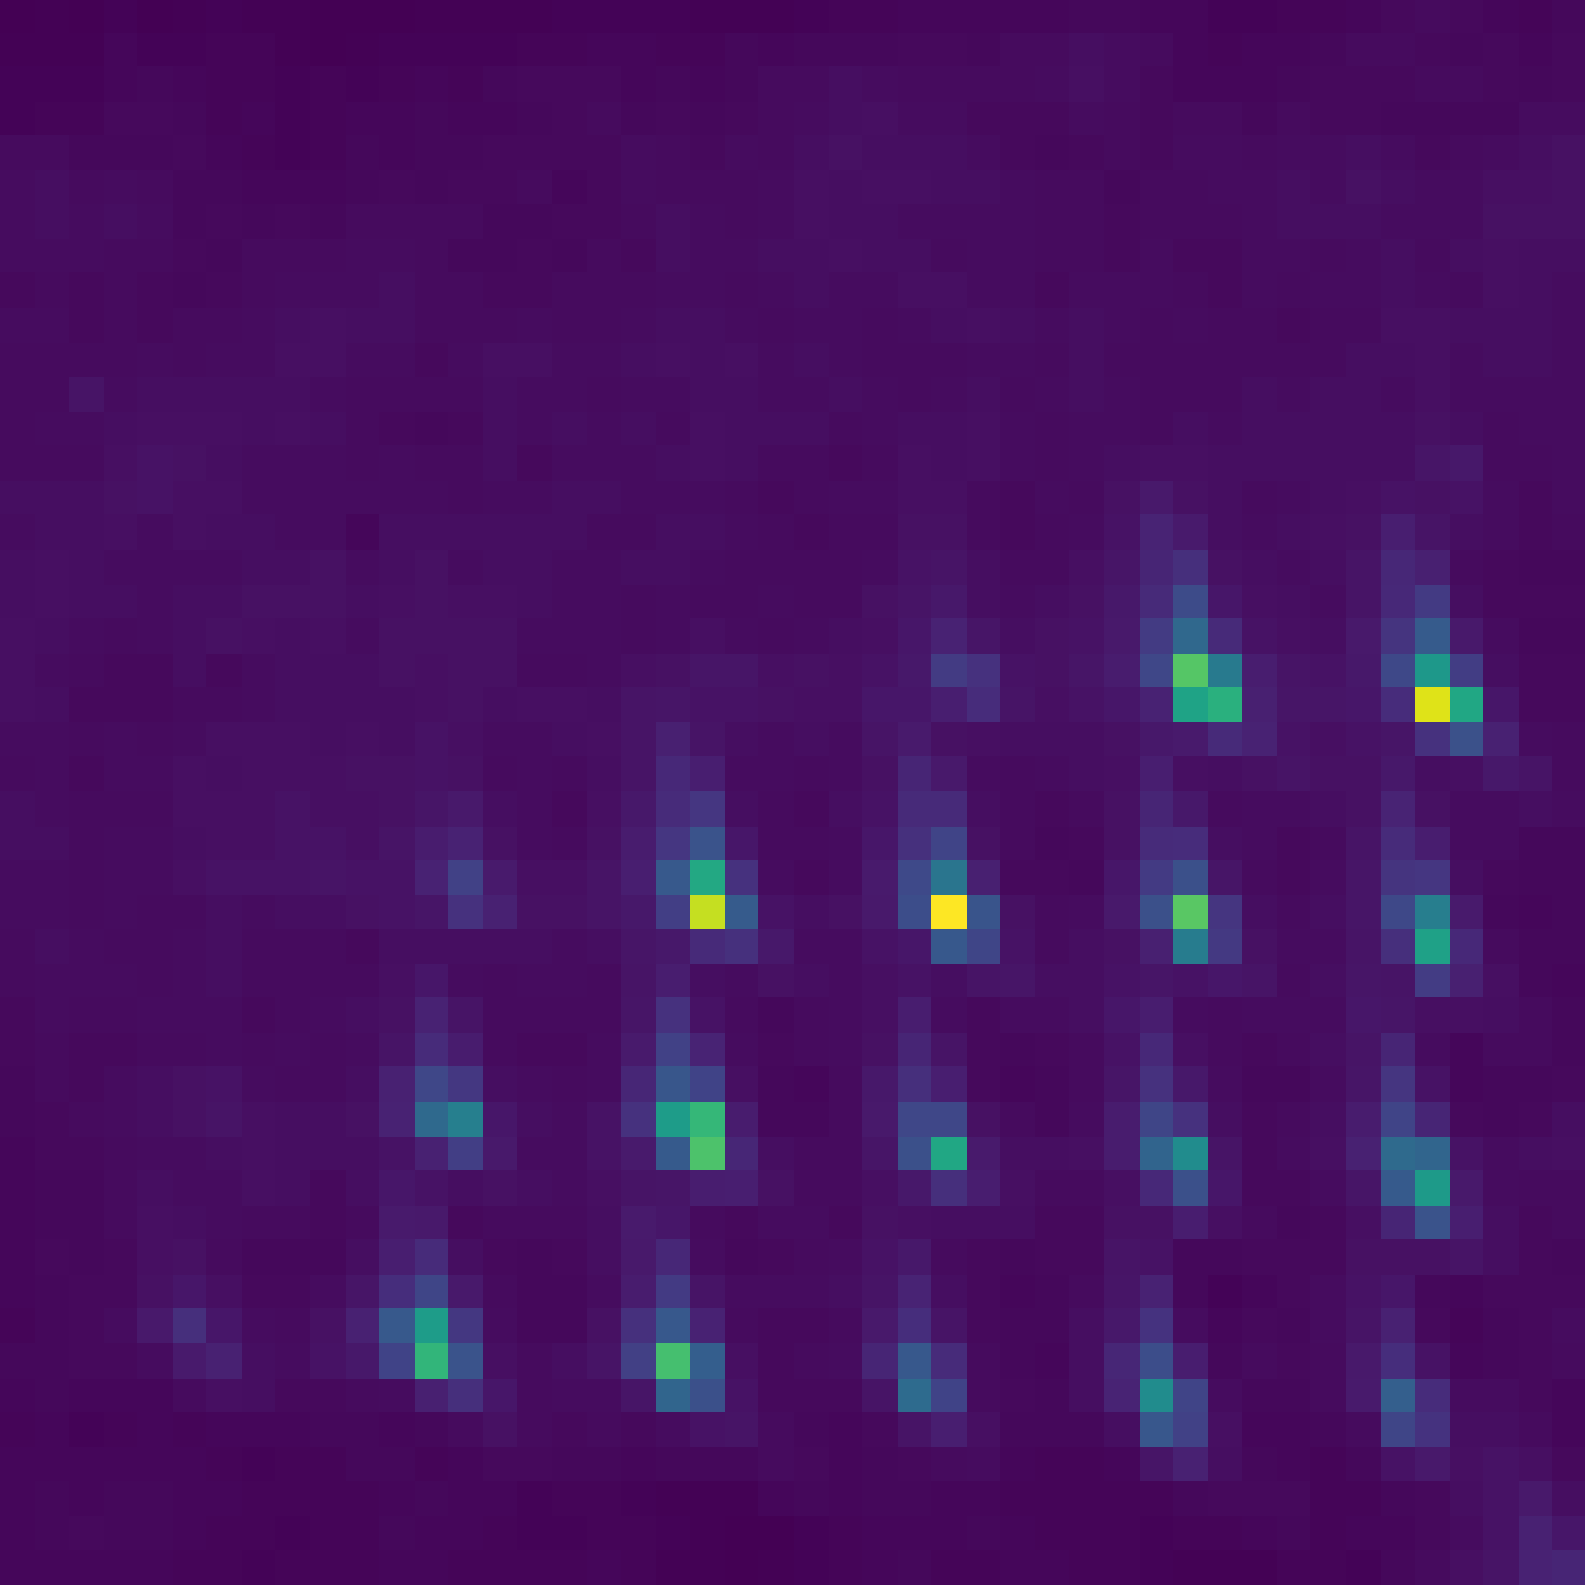
\includegraphics[width=1.4in] {grid6x62blue.pdf}};;
		\draw[white] (-1.05,-0.55) rectangle (1.70,0.05);
		\draw[white, fill=white] (0.95,1.4) rectangle (1.45,1.45);
\node[color=white] at (1.03,1.1) {\footnotesize \SI{20}{\micro\meter}};
		\end{tikzpicture}
		\centering
		\caption{}
		\label{36c}
	\end{subfigure}
	\caption{(a) Recorded light intensity in the trapping plane. (b) Corresponding grid of optical power per trap in \si{\milli\watt}. (c) Integrated atom fluorescence. The box marks the 5 traps used for analysis of the ac-Stark shift (see \autoref{stark}). The $\sfrac{1}{\mathrm{e}^2}$ diameter of the traps is \SI{2.2}{\micro\meter}.}
	\label{mainstarkfigure}
\end{figure}
Calibration of the CCD camera enables the extraction of absolute optical power per trap (\autoref{36b}). The recorded fluorescence (\autoref{36c}, integration time: \SI{1667}{\second}) shows that on average, the deepest half of the trapping sites is occupied.


We record the fluorescence for each site by imaging the atom onto an EMCCD. The fluorescence count rate is measured for each trap over a \SI{30}{\milli\second} exposure (frame) for a total of $50\,000$ frames. Measurements of the five trapping sites indicated in \autoref{36c} are shown in \autoref{masterplot}.

\begin{figure}[h!]
	\centering
	\begin{tikzpicture}
		
		\begin{groupplot}[group style={group size=3 by 5,horizontal sep=0.72cm, vertical sep=0.72cm},xmin=0,ymin=0,height=4cm,width=4cm,no markers]
			\nextgroupplot
			[
			title={\small$P=\SI{15}{\milli\watt}$},
			title style={yshift=-0.24cm},
			xmin=0, xmax=250,
			ymin=-100/1000, ymax=600/1000,
			%xtick={0,20,40,60,80,100},
			%ytick={0,20,40,60,80,100,120},
			%legend pos=north west,
			xticklabels={,,},
			xmajorgrids=true,
			ymajorgrids=true,
			grid style=dashed,
			y label style={at={(axis description cs:-0.1,0.5)},anchor=south},
			x tick label style={rotate=0},
			width=7cm,
			]
			
			\addplot[
			color=markrood
			] table [col sep = comma, x index = 0, y expr=\thisrowno{1}*1.3062923961932331*9/1000/1000/0.033]{TRACE19b.csv};
			
			\nextgroupplot
			[
			%title={Temperature dependence of CuSO$_4\cdot$5H$_2$O solubility},
			xmin=-100/1000, xmax=600/1000,
			%ymin=0, ymax=120,
			%ytick={0,20,40,60,80,100,120},
			%legend pos=north west,
			%ymajorgrids=true,
			xticklabels={,,},
			xmajorgrids=true,
			grid style=dashed,
			y label style={at={(axis description cs:0.30,.5)},anchor=south},
			x tick label style={rotate=90}
			]
			
			\addplot[
			ybar,
			bar width=1.1pt,
			bar shift=0.55pt,
			fill=markgrijs,
			draw=markgrijs,
			mark = *,
			color=markgrijs,
			opacity=0.5
			] table [col sep = comma, x expr=\thisrowno{0}*1.3062923961932331*9/1000/1000/0.033, y index = 1]{FLUORhist19.csv};
			
			\addplot[
			color=markrood,
			style={thick}
			] table [col sep = comma, x expr=\thisrowno{0}*1.3062923961932331*9/1000/1000/0.033, y index = 1]{FLUORFIThist19.csv};
			
			\node[anchor=north] (source) at (axis cs:1295*1.3062923961932331*9/1000/1000/0.033,0.003){};
			\draw[-latex, color=markrood](source)--++(0cm, -0.5cm);
			
			\nextgroupplot
			[
			%title={Temperature dependence of CuSO$_4\cdot$5H$_2$O solubility},
			xmin=-0, xmax=10,
			%ymin=0, ymax=120,
			%ytick={0,20,40,60,80,100,120},
			%legend pos=north west,
			%ymajorgrids=true,
			xticklabels={,,},
			xmajorgrids=true,
			grid style=dashed,
			y label style={at={(axis description cs:0.30,.5)},anchor=south},
			x tick label style={rotate=90},
			scaled y ticks={base 10:2}
			]
			
			\addplot[
			ybar,
			bar width=1.1pt,
			bar shift=0.55pt,
			fill=markgrijs,
			draw=markgrijs,
			mark = *,
			color=markgrijs,
			opacity=0.5
			] table [col sep = comma, x expr=\thisrowno{0}/30, y expr=\thisrowno{1}]{LIFEhist19.csv};
			
			\addplot[
			color=markrood,
			style={thick}
			] table [col sep = comma, x expr=\thisrowno{0}/30, y index = 1]{LIFEFIThist19.csv};
			
			\node at (1.25cm,2.2cm) {\footnotesize ${\tau}=0.38\pm0.04\,$s};
			
			\nextgroupplot
			[
			title={\small$P=\SI{20}{\milli\watt}$},
			title style={yshift=-0.24cm},
			xmin=0, xmax=250,
			ymin=-100/1000, ymax=600/1000,
			%xtick={0,20,40,60,80,100},
			%ytick={0,20,40,60,80,100,120},
			%legend pos=north west,
			xticklabels={,,},
			xmajorgrids=true,
			ymajorgrids=true,
			grid style=dashed,
			y label style={at={(axis description cs:-0.1,.5)},anchor=south},
			x tick label style={rotate=0},
			width=7cm,
			]
			
			\addplot[
			color=markrood
			] table [col sep = comma, x index = 0, y expr=\thisrowno{1}*1.3062923961932331*9/1000/1000/0.033]{TRACE20b.csv};
			
			\nextgroupplot
			[
			%title={Temperature dependence of CuSO$_4\cdot$5H$_2$O solubility},
			xmin=-100/1000, xmax=600/1000,
			%ymin=0, ymax=120,
			%ytick={0,20,40,60,80,100,120},
			%legend pos=north west,
			%ymajorgrids=true,
			xticklabels={,,},
			xmajorgrids=true,
			grid style=dashed,
			x tick label style={rotate=90}
			]
			
			\addplot[
			ybar,
			bar width=1.1pt,
			bar shift=0.55pt,
			fill=markgrijs,
			draw=markgrijs,
			mark = *,
			color=markgrijs,
			opacity=0.5
			] table [col sep = comma, x expr=\thisrowno{0}*1.3062923961932331*9/1000/1000/0.033, y index = 1]{FLUORhist20.csv};
			
			\addplot[
			color=markrood,
			style={thick}
			] table [col sep = comma, x expr=\thisrowno{0}*1.3062923961932331*9/1000/1000/0.033, y index = 1]{FLUORFIThist20.csv};
			
			\node[anchor=north] (source) at (axis cs:968*1.3062923961932331*9/1000/1000/0.033,0.004){};
			\draw[-latex, color=markrood](source)--++(0cm, -0.5cm);
			
			\nextgroupplot
			[
			%title={Temperature dependence of CuSO$_4\cdot$5H$_2$O solubility},
			xmin=-0, xmax=10,
			%ymin=0, ymax=120,
			%ytick={0,20,40,60,80,100,120},
			%legend pos=north west,
			%ymajorgrids=true,
			xticklabels={,,},
			xmajorgrids=true,
			grid style=dashed,
			y label style={at={(axis description cs:0.30,.5)},anchor=south},
			x tick label style={rotate=90}
			]
			
			\addplot[
			ybar,
			bar width=1.1pt,
			bar shift=0.55pt,
			fill=markgrijs,
			draw=markgrijs,
			mark = *,
			color=markgrijs,
			opacity=0.5
			] table [col sep = comma, x expr=\thisrowno{0}/30, y index = 1]{LIFEhist20.csv};
			
			\addplot[
			color=markrood,
			style={thick}
			] table [col sep = comma, x expr=\thisrowno{0}/30, y index = 1]{LIFEFIThist20.csv};
			
			\node at (1.25cm,2.2cm) {\footnotesize ${\tau}=3.6\pm0.6\,$s};
			
			\nextgroupplot
			[
			title={\small$P=23\,$\si{\milli\watt}},
			title style={yshift=-0.24cm},
			ylabel={Fluorescence counts (\si{\mega\hertz})},
			xmin=0, xmax=250,
			ymin=-100/1000, ymax=600/1000,
			%xtick={0,20,40,60,80,100},
			%ytick={0,20,40,60,80,100,120},
			%legend pos=north west,
			xticklabels={,,},
			xmajorgrids=true,
			ymajorgrids=true,
			grid style=dashed,
			y label style={at={(axis description cs:-0.12,.5)},anchor=south},
			x tick label style={rotate=0},
			width=7cm,
			]
			
			\addplot[
			color=markrood
			] table [col sep = comma, x index = 0, y expr=\thisrowno{1}*1.3062923961932331*9/1000/1000/0.033]{TRACE21b.csv};
			
			\nextgroupplot
			[
			%title={Temperature dependence of CuSO$_4\cdot$5H$_2$O solubility},
			xmin=-100/1000, xmax=600/1000,
			%ymin=0, ymax=120,
			%ytick={0,20,40,60,80,100,120},
			%legend pos=north west,
			%ymajorgrids=true,
			xticklabels={,,},
			xmajorgrids=true,
			grid style=dashed,
			x label style={at={(axis description cs:0.5,-.3)},anchor=south},
			x tick label style={rotate=90}
			]
			
			\addplot[
			ybar,
			bar width=1.1pt,
			bar shift=0.55pt,
			fill=markgrijs,
			draw=markgrijs,
			mark = *,
			color=markgrijs,
			opacity=0.5
			] table [col sep = comma, x expr=\thisrowno{0}*1.3062923961932331*9/1000/1000/0.033, y index = 1]{FLUORhist21.csv};
			
			\addplot[
			color=markrood,
			style={thick}
			] table [col sep = comma, x expr=\thisrowno{0}*1.3062923961932331*9/1000/1000/0.033, y index = 1]{FLUORFIThist21.csv};
			
			\node[anchor=north] (source) at (axis cs:794*1.3062923961932331*9/1000/1000/0.033,0.0042){};
			\draw[-latex, color=markrood](source)--++(0cm, -0.5cm);
			
			\nextgroupplot
			[
			%title={Temperature dependence of CuSO$_4\cdot$5H$_2$O solubility},
			xmin=-0, xmax=10,
			%ymin=0, ymax=120,
			%ytick={0,20,40,60,80,100,120},
			%legend pos=north west,
			%ymajorgrids=true,
			xticklabels={,,},
			xmajorgrids=true,
			grid style=dashed,
			y label style={at={(axis description cs:0.30,.5)},anchor=south},
			x tick label style={rotate=90}
			]
			
			\addplot[
			ybar,
			bar width=1.1pt,
			bar shift=0.55pt,
			fill=markgrijs,
			draw=markgrijs,
			mark = *,
			color=markgrijs,
			opacity=0.5
			] table [col sep = comma, x expr=\thisrowno{0}/30, y index = 1]{LIFEhist21.csv};
			
			\addplot[
			color=markrood,
			style={thick}
			] table [col sep = comma, x expr=\thisrowno{0}/30, y index = 1]{LIFEFIThist21.csv};
			
			\node at (1.25cm,2.2cm) {\footnotesize ${\tau}=5.6\pm1.0\,$s};
			
			\nextgroupplot
			[
			title={\small$P=\SI{24}{\milli\watt}$},
			title style={yshift=-0.24cm},
			xmin=0, xmax=250,
			ymin=-100/1000, ymax=600/1000,
			%xtick={0,20,40,60,80,100},
			%ytick={0,20,40,60,80,100,120},
			%legend pos=north west,
			xticklabels={,,},
			xmajorgrids=true,
			ymajorgrids=true,
			grid style=dashed,
			y label style={at={(axis description cs:-0.1,.5)},anchor=south},
			x tick label style={rotate=0},
			width=7cm,
			]
			
			\addplot[
			color=markrood
			] table [col sep = comma, x index = 0, y expr=\thisrowno{1}*1.3062923961932331*9/1000/1000/0.033]{TRACE22b.csv};
			
			\nextgroupplot
			[
			%title={Temperature dependence of CuSO$_4\cdot$5H$_2$O solubility},
			xmin=-100/1000, xmax=600/1000,
			%ymin=0, ymax=120,
			%ytick={0,20,40,60,80,100,120},
			%legend pos=north west,
			%ymajorgrids=true,
			xticklabels={,,},
			xmajorgrids=true,
			grid style=dashed,
			x tick label style={rotate=90}
			]
			
			\addplot[
			ybar,
			bar width=1.1pt,
			bar shift=0.55pt,
			fill=markgrijs,
			draw=markgrijs,
			mark = *,
			color=markgrijs,
			opacity=0.5
			] table [col sep = comma, x expr=\thisrowno{0}*1.3062923961932331*9/1000/1000/0.033, y index = 1]{FLUORhist22.csv};
			
			\addplot[
			color=markrood,
			style={thick}
			] table [col sep = comma, x expr=\thisrowno{0}*1.3062923961932331*9/1000/1000/0.033, y index = 1]{FLUORFIThist22.csv};
			
			\node[anchor=north] (source) at (axis cs:703*1.3062923961932331*9/1000/1000/0.033,0.0045){};
			\draw[-latex, color=markrood](source)--++(0cm, -0.5cm);
			
			\nextgroupplot
			[
			%title={Temperature dependence of CuSO$_4\cdot$5H$_2$O solubility},
			xmin=-0, xmax=10,
			%ymin=0, ymax=120,
			%ytick={0,20,40,60,80,100,120},
			%legend pos=north west,
			%ymajorgrids=true,
			xticklabels={,,},
			xmajorgrids=true,
			grid style=dashed,
			y label style={at={(axis description cs:0.30,.49)},anchor=south},
			x tick label style={rotate=90}
			]
			
			\addplot[
			ybar,
			bar width=1.1pt,
			bar shift=0.55pt,
			fill=markgrijs,
			draw=markgrijs,
			mark = *,
			color=markgrijs,
			opacity=0.5
			] table [col sep = comma, x expr=\thisrowno{0}/30, y index = 1]{LIFEhist22.csv};
			
			\addplot[
			color=markrood,
			style={thick}
			] table [col sep = comma, x expr=\thisrowno{0}/30, y index = 1]{LIFEFIThist22.csv};
			
			\node at (1.25cm,2.2cm) {\footnotesize ${\tau}=5.3\pm1.0\,$s};
	
			\nextgroupplot
			[
			title={\small$P=\SI{29}{\milli\watt}$},
			title style={yshift=-0.24cm},
			xlabel={Time (s)},
			xmin=0, xmax=250,
			ymin=-100/1000, ymax=600/1000,
			%xtick={0,20,40,60,80,100},
			%ytick={0,20,40,60,80,100,120},
			%legend pos=north west,
			xmajorgrids=true,
			ymajorgrids=true,
			grid style=dashed,
			y label style={at={(axis description cs:-0.1,0.5)},anchor=south},
			x label style={at={(axis description cs:0.5,-.5)},anchor=south},
			x tick label style={rotate=0},
			width=7cm,
			]
			
			\addplot[
			color=markrood
			] table [col sep = comma, x index = 0, y expr=\thisrowno{1}*1.3062923961932331*9/1000/1000/0.033]{TRACE23b.csv};
			
			\nextgroupplot
			[
			%title={Temperature dependence of CuSO$_4\cdot$5H$_2$O solubility},
			xlabel = {Counts (\si{\mega\hertz})},
			xmin=-100/1000, xmax=600/1000,
			%ymin=0, ymax=1600,
			%xtick={0,20,40,60,80,100},
			%ytick={0,20,40,60,80,100,120},
			%legend pos=north west,
			%ymajorgrids=true,
			xmajorgrids=true,
			grid style=dashed,
			x tick label style={rotate=0},
			y label style={at={(axis description cs:-0.1,.5)},anchor=south},
			x label style={at={(axis description cs:0.5,-.5)},anchor=south},
			]
			
			\addplot[
			ybar,
			bar width=1.1pt,
			bar shift=0.55pt,
			fill=markgrijs,
			draw=markgrijs,
			mark = *,
			color=markgrijs,
			opacity=0.5
			] table [col sep = comma, x expr=\thisrowno{0}*1.3062923961932331*9/1000/1000/0.033, y index = 1]{FLUORhist23.csv};
			
			\addplot[
			color=markrood,
			style={thick}
			] table [col sep = comma, x expr=\thisrowno{0}*1.3062923961932331*9/1000/1000/0.033, y index = 1]{FLUORFIThist23.csv};
			
			\node[anchor=north] (source) at (axis cs:422*1.3062923961932331*9/1000/1000/0.033,0.005){};
			\draw[-latex, color=markrood](source)--++(0.0cm, -0.5cm);
			
			\nextgroupplot
			[
			%title={Temperature dependence of CuSO$_4\cdot$5H$_2$O solubility},
			xmin=-0, xmax=10,
			%ymin=0, ymax=120,
			%ytick={0,20,40,60,80,100,120},
			%legend pos=north west,
			%ymajorgrids=true,
			%xticklabels={,,},
			xmajorgrids=true,
			grid style=dashed,
			y label style={at={(axis description cs:0.30,.5)},anchor=south},
			x tick label style={rotate=0},
			xlabel = {Lifetime (s)},
			x label style={at={(axis description cs:0.5,-.5)},anchor=south},
			]
			
			\addplot[
			ybar,
			bar width=1.1pt,
			bar shift=0.55pt,
			fill=markgrijs,
			draw=markgrijs,
			mark = *,
			color=markgrijs,
			opacity=0.5
			] table [col sep = comma, x expr=\thisrowno{0}/30, y index = 1]{LIFEhist23.csv};
			
			\addplot[
			color=markrood,
			style={thick}
			] table [col sep = comma, x expr=\thisrowno{0}/30, y index = 1]{LIFEFIThist23.csv};
			
			\node at (1.25cm,2.2cm) {\footnotesize ${\tau}=6.1\pm0.6\,$s};
			
		\end{groupplot}
		
	\end{tikzpicture}
	\caption[An example of a floating figure]{(Left column) Fluorescence count rate from 5 traps of varying optical power corrected for background counts and EMCCD quantum efficiency. (Middle column) Normalised histogram and multimodal MLE fit of the fluorescence count rate acquired over a period of \SI{1667}{\second}. (Right column) Normalised histogram and exponential MLE fit of the trap lifetime.} % The text in the square bracket is the caption for the list of figures while the text in the curly brackets is the figure caption
	\label{masterplot} 
\end{figure}



The count rates per frame are corrected for background counts and the EMCCD quantum efficiency ($44\%$). The histogram of binned count rates reveals the discretisation that is directly related to the number of atoms occupying the trap. Except for the deepest trap in this series, which shows up to triple atom occupation, all traces reveal two distinct peaks. Whereas the first is associated with the background count rate, the second peak (for which the fluorescence is brighter) corresponds tot the fluorescence of a single atom. Bimodal distributions are fitted to these histograms using maximum likelihood estimation (MLE), which estimates the parameters of a distribution by maximising a likelihood function, such that the observed data is most probable under the assumed statistical model. Single atom occupation is a result of the collisional blockade mechanism \cite{Schlosser2002}: when the trap volume is small enough, multi-atom collisions become the dominant loss mechanism in the trap. Consequently, if one neglects the single-body loss rate, the length of the dark and bright intervals of the fluorescence trace are equal, as the arrival of an atom either triggers a loading or loss event. If we consider such events realisations of a homogeneous Poisson process, the time differences between events, i.\,e. the lengths of bright (or dark) intervals, are exponentially distributed ($\sim\lambda \mathrm{e}^{-\lambda x}$) with mean lifetime $\tau=\sfrac{1}{\lambda}$. This data and the MLE fitted exponential distributions are shown in \autoref{masterplot}.
\begin{figure}[h]
	\centering
	\begin{tikzpicture}
	
	\begin{axis}
	[
	%title={Temperature dependence of CuSO$_4\cdot$5H$_2$O solubility},
	ylabel={Fluorescence counts (\si{\mega\hertz})},
	xlabel={Dipole trap power (\si{\milli\watt})},
	xmin=0, xmax=35,
	%ymin=0, ymax=120,
	%xtick={0,20,40,60,80,100},
	%ytick={0,20,40,60,80,100,120},
	%legend pos=north west,
	ymajorgrids=false,
	grid style=dashed,
	%y label style={at={(axis description cs:0.30,.5)},anchor=south},
	%x tick label style={rotate=90}
	height=5.5cm,
	width=5.5cm,
	name=mainplot,
	ymajorgrids=true,
	xmajorgrids=true
	]

	
	\draw[dashed,help lines] (axis cs:0,0) -- (axis cs:35,0);
	
	
	\addplot[
	only marks,
	draw=markgrijs,
	mark = *,
	color=markgrijs,
	opacity=1
	] table [col sep = comma, x index = 0, y expr = \thisrowno{1}/1e6, y error expr = \thisrowno{2}/1e6]{fluor.csv};
	

	
	
	\addplot[
	color=markrood,
	style={thick},
	name path=plot0
	] table [col sep = comma, x index = 0, y expr = \thisrowno{1}/1e6]{fluorfit.csv};
	
	\addplot[
	color=markrood,
	style={ultra thin},
	name path=plotm
	] table [col sep = comma, x index = 0, y expr = \thisrowno{1}/1e6]{fluorfit2m.csv};
	
	\addplot[
	color=markrood,
	style={ultra thin},
	name path=plotmm
	] table [col sep = comma, x index = 0, y expr = \thisrowno{1}/1e6]{fluorfit4m.csv};
	
	\addplot[
	color=markrood,
	style={ultra thin},
	name path=plotmmm
	] table [col sep = comma, x index = 0, y expr = \thisrowno{1}/1e6]{fluorfit6m.csv};	
	
	\addplot[
	color=markrood,
	style={ultra thin},
	name path=plotp
	] table [col sep = comma, x index = 0, y expr = \thisrowno{1}/1e6]{fluorfit2p.csv};	
	
	\addplot[
	color=markrood,
	style={ultra thin},
	name path=plotpp
	] table [col sep = comma, x index = 0, y expr = \thisrowno{1}/1e6]{fluorfit4p.csv};
	
	\addplot[
	color=markrood,
	style={ultra thin},
	name path=plotppp
	] table [col sep = comma, x index = 0, y expr = \thisrowno{1}/1e6]{fluorfit6p.csv};
	
	\addplot[markrood, opacity=0.05] fill between[
	of = plotpp and plotppp,
	]; 
	
	\addplot[markrood, opacity=0.2] fill between[
	of = plotp and plotpp,
	]; 
	
	\addplot[markrood, opacity=0.35] fill between[
	of = plot0 and plotp,
	]; 
	
	\addplot[markrood, opacity=0.35] fill between[
	of = plotm and plot0,
	]; 
	
	\addplot[markrood, opacity=0.2] fill between[
	of = plotmm and plotm,
	]; 
	
	\addplot[markrood, opacity=0.05] fill between[
	of = plotmmm and plotmm,
	]; 
	
	
	\end{axis}
	
	\end{tikzpicture}
	\caption[An example of a floating figure]{Fluorescence count rate versus optical dipole trap power. The red line is a fit based on the calculated scattering rate, which is corrected for the solid angle of light collection (\SI{10}{\percent} of $4\pi\,$sr) and reflectivity of the dichroic mirror (\SI{90}{\percent}, see \autoref{setup}). (Inset) Expansion of the shaded region. Bands around the central fit correspond to multiples of the standard deviation ($\pm2\sigma$, $\pm4\sigma$, $\pm6\sigma$) of the fit parameter $\alpha=\SI{0.6}{\percent}$.} % The text in the square bracket is the caption for the list of figures while the text in the curly brackets is the figure caption
	\label{starkfig} 
\end{figure}
The extracted mean lifetimes shall be further discussed in \autoref{lifetimeandfilling} as part of a larger dataset. Returning to the fluorescence count rate analysis, we observe that the single atom count rate decreases with deeper traps. Due to the ac-Stark effect, the energy levels of the cooling transition are shifted further away from the cooling light for atoms in stronger light fields, which reduces the scattering rate. For far detuned\footnote{Assuming a resolved fine-structure (spin-orbit coupling), but unresolved hyperfine structure (coupling to nuclear spin). The atom-field interaction is thus considered in terms of the electronic angular momentum configuration of the $\mathrm{D}1$ and $\mathrm{D}2$ line: $J=\sfrac{1}{2} \rightarrow J' =\sfrac{1}{2},\sfrac{3}{2}$.}, linearly polarised light with intensity $I(\vec{r}\,)$, the ground state of \ce{^87Rb} is shifted in energy by
\begin{equation}
\label{starkequation}
\Delta E_\text{g}(\vec{r}\,) = \frac{\pi c^2}{2}\left( \frac{2\Gamma_2}{\omega_{0,2}^3\Delta_2} + \frac{\Gamma_1}{\omega_{0,1}^3\Delta_1}\right) I(\vec{r}\,)	\,,
\end{equation}
where $\Gamma_i$, $\omega_{0,i}$ and $\Delta_i$ denote the properties of the $D_i$ line \cite{Grimm2000}. The peak intensity of a trap can be calculated from the optical power $P$ and the trap waist $w_0$ in the focal plane, given by $w_0=2M^2 \lambda f/\pi D$, which depends on the beam propagation faction $M^2=1.6$, lens focal length $f=30\,$mm and the $\sfrac{1}{\mathrm{e}^2}$ diameter $D=\SI{30}{\milli\meter}$ of the incident beam. With this information, we obtain a maximum ground state shift of $\Delta E_g/\hbar P=-2\pi\times \SI{1.49}{\mega\hertz\per\milli\watt}$. The excited level \ce{5\!^2P_{\sfrac{3}{2}}} shifts in the opposite direction by an amount that equals the corresponding term in \autoref{starkequation}: $\Delta E_e/\hbar P=2\pi\times \SI{0.97}{\mega\hertz\per\milli\watt}$. The total differential light shift $\Delta E_\text{diff}=\Delta E_e-\Delta E_g$ of the cooling transition is thus given by $\Delta E_\text{diff}/\hbar P=2\pi\times \SI{2.47}{\mega\hertz\per\milli\watt}$. In this case, the scattering rate is given by \autoref{scatter} with a detuning that is now adjusted for the ac-Stark effect and a saturation intensity $I_\text{sat}=\SI{3.58}{\milli\watt\per\square\centi\meter}$ that corresponds to an isotropic pump field driving the $\ket{F=2}\rightarrow\ket{F'=3}$ cycling transition, ignoring scattering from light tuned to the $\ket{F=1}\rightarrow\ket{F'=2}$ repump transition \cite{steck}. In addition, we ignore the magnetic field and assume that on average, the atoms are illuminated by all polarisations with a total intensity of $6I_0$, where $I_0=\SI{11.3}{\milli\watt\per\centi\meter^2}$ is the maximum intensity of a single MOT beam. \autoref{starkfig} shows the measured fluorescence count rate versus dipole trap power extracted from \autoref{masterplot}. The fit is based on the calculated scattering rate and is corrected for the emission into the solid angle of the lens (\SI{10}{\percent}) and reflectivity of the dichroic mirror (\SI{90}{\percent}). The only free parameter $\alpha\in[0,1]$ accounts for a reduced intensity of the cooling light ($6I_0\rightarrow6\alpha I_0$) at the position of the dipole trap, which is shifted with respect to the centre of the MOT. Note that in a trap with a reasonable lifetime (\autoref{masterplot}), the ac-Stark effect is responsible for a significant reduction of the fluorescence count rate with respect to the unperturbed atom ($P=0$).

\subsection{Trap lifetime and filling fraction}
\label{lifetimeandfilling}
For an analysis of trap lifetime and filling fraction we consider all trapping sites in \autoref{c} that exhibit a clear sign of single atom occupation based on the recorded fluorescence count rate. A bimodal distribution is fitted to all realisations of the fluorescence count rate (as in \autoref{masterplot}), which is repeated for a series of three measurements ($50\,000$ frames each). Each fit sets the cut-off rate (defined as the mean of the bimodal peak positions) above which the trap is considered to be filled (bright).
\begin{figure}[!t]
	%\vspace{0.7em}
	\centering
	\begin{tikzpicture}
	
	\begin{groupplot}[group style={group size=2 by 1, horizontal sep=2.5cm},xmin=0,ymin=0,height=5.5cm,width=5.5cm,no markers]
	\nextgroupplot
	[
	%title={Temperature dependence of CuSO$_4\cdot$5H$_2$O solubility},
	xlabel={Power in dipole trap (\si{\milli\watt})},
	ylabel={Average trap lifetime (s)},
	%xmin=0, xmax=100,
	%ymin=0, ymax=120,
	%xtick={0,20,40,60,80,100},
	%ytick={0,20,40,60,80,100,120},
	%legend pos=north west,
	ymajorgrids=true,
	xmajorgrids=true,
	grid style=dashed,
	]
	
	\addplot[
	only marks,
	mark = *,
	color=markrood,
	/pgfplots/error bars/.cd,
	y dir = both,
	y explicit,
	] table [col sep = comma, x index = 0, y index = 1, y error index = 2]{LT.csv};
	\iffalse
	\draw[dashed,markrood] (10.606060606060607, 0) -- (10.606060606060607, 13);
	\draw[dashed,markrood] (24.50757575757576, 0) -- (24.50757575757576, 13);
	\draw[->,>=stealth,markgrijs] (10.606060606060607, 3) -- (24.50757575757576, 3);
	\node[markgrijs] at (10.606060606060607-3,3) {$A$};
	\node[markgrijs] at (24.50757575757576+3,3) {$B$};
	\fi
	%\legend{CuSO$_4\cdot$5H$_2$O}
	
	\nextgroupplot
	[
	%title={Temperature dependence of CuSO$_4\cdot$5H$_2$O solubility},
	xlabel={Power in dipole trap (\si{\milli\watt})},
	ylabel={Filling fraction},
	%xmin=0, xmax=100,
	%ymin=0, ymax=120,
	%xtick={0,20,40,60,80,100},
	%ytick={0,20,40,60,80,100,120},
	legend pos=north west,
	ymajorgrids=true,
	xmajorgrids=true,
	grid style=dashed,
	]
	
	\addplot[
	only marks,
	mark = *,
	color=markrood,
	/pgfplots/error bars/.cd,
	y dir = both,
	y explicit,
	] table [col sep = comma, x index = 0, y index = 1, y error index = 2]{FR.csv};
	
	\iffalse
	\draw[dashed,markrood] (10.606060606060607, 0) -- (10.606060606060607, 13);
	\draw[dashed,markrood] (24.50757575757576, 0) -- (24.50757575757576, 13);
	\draw[->,>=stealth,markgrijs] (10.606060606060607, 0.25) -- (24.50757575757576, 0.25);
	\node[markgrijs] at (10.606060606060607-3,0.25) {$A$};
	\node[markgrijs] at (24.50757575757576+3,0.25) {$B$};
	\fi
	
	%\legend{CuSO$_4\cdot$5H$_2$O}
	
	\end{groupplot}
	
	\end{tikzpicture}
	\caption[An example of a floating figure]{Average trap lifetime (left) and filling fraction (right) versus dipole trap power. Error bars represent the standard error of the mean based on up to three measurements of the fluorescence count rate ($50\,000$ frames) per trapping site.} % The text in the square bracket is the caption for the list of figures while the text in the curly brackets is the figure caption
	\label{fig:LTandFR} 
\end{figure}
These cut-off values are then used to calculate the average trap lifetime (i.\,e. the mean duration of bright fluorescence intervals) and trap filling fraction (i.\,e. the fraction of measurement time for which the trap is filled). The results are shown in \autoref{fig:LTandFR}. First note that the filling fraction reaches a plateau around \SI{50}{\percent} for trap powers above \SI{20}{\milli\watt}. An explanation for this phenomenon is the dominance of the two-body loss rate in the collisional blockade regime, which implies that the single-body loss effect is negligible and the average lengths of the bright and dark intervals are equal because the loading and loss are equally probable. For low powers, the atoms are more likely to be ejected from the shallow trapping potential due to heating, background gas collisions and the energy distribution of the atom. The effect is a reduced filling fraction and average trap lifetime, which agrees with the visible trend in \autoref{fig:LTandFR}.

\iffalse
\section{Dipole-trapping theory}

Our work relies on exploiting the dipole interaction between atoms and light in order to trap individual atoms at the intensity maximum of a focused red-detuned laser. Dipole-force traps are conservative, therefore to trap atoms in this way requires them to be pre-cooled; a Magneto-Optical Trap (MOT) is typically used from which to load atoms. 

There are two mechanisms by which atoms are lost from such a dipole trap. The first is via a collision with a background atom that imparts sufficient kinetic energy for the atom's energy to exceed the depth of the trap. The second loss mechanism comes into play when there is more than one atom in the trap; this mechanism is a light-assisted collision between two trapped atoms \cite{fuhrmanek2012}, and it causes both of the atoms involved to be lost from the trap. The smaller the waist of a dipole trap, the more dominant the light-assisted loss channel becomes. 

Under some critical trap volume (the value of which is determined experimentally, but typically corresponds to a trap waist of the order of \SI{1}{\micro\metre} \cite{fung2015a}) these light-assisted collisions dominate the loss as soon as there are two atoms in the trap \cite{schlosser2002a}. In this case it is guaranteed that the trap will contain either zero or one atoms at any given time. In the limit that this loss mechanism dominates entirely, the average atom number is locked to \num{0.5} and is insensitive to fluctuations in the trap loading rate. In practice, other loss mechanisms persist, so this \SI{50}{\percent} occupation actually serves as an upper bound.

The potential experienced by an \ce{^87Rb} atom, cooled on the $\mathrm{D}2$ transition, held in a far-detuned optical dipole trap of intensity $I$ is given by
\begin{equation}\label{eq:dipPot}
U_{\mathrm{dip}} \approx \frac{\hbar\Gamma^2}{8\Delta}\frac{I}{I_{\mathrm{sat}}},
\end{equation}
where the assumption has been made that the detuning $\Delta$ of the trapping light is sufficiently large as to neglect the different detunings from the $\mathrm{D}1$ and $\mathrm{D}2$ lines. Here, $I_{\mathrm{sat}}$ is the saturation intensity and $\Gamma$ is the linewidth of the $\mathrm{D}2$ transition. It should be noted that for red detuning, $\Delta$ is negative and so the potential is attractive.  

Thus the presence of the trapping light results in a Stark shift to the energy levels of a trapped atom, which affects its interaction with the light that is used to cool it in the MOT. As such, different depths of dipole traps and different detunings of the MOT cooling light from resonance will affect how a dipole trap behaves in terms of how readily single atoms are loaded into it and how quickly they are lost from it. For a given MOT detuning, a shallower trap will provide a smaller Stark shift and hence a higher scattering rate, leading to a higher loading rate and better cooling. A deeper trap will give a larger Stark shift and hence a lower scattering rate, resulting in a lower loss rate for atoms in the trap. 

\fi


\iffalse
\section{Experimental arrangement}
%put in vacuum pressure (at end of first para?)

We use \ce{^{87}Rb} atoms, cooled on the $\mathrm{D}2$ transition (\SI{780.246}{\nm}). We dipole-trap single atoms using light at \SI{1064}{\nm}. This large red detuning helps to minimise scattering of the trapping light by the atom. The traps are formed with a waist of  \SI{1.6}{\um}, with depths of the order of hundreds of \SI{}{MHz}.

The atoms are loaded into the traps from a MOT. The MOT is formed using $3$ retro-reflected cooling beams with total power \SI{8}{\milli\watt} and re-pumping light on the $\ce{^2S_{1/2}} (F=1) \, \rightarrow \, \ce{^2P_{3/2}} (F'=2)$ transition with approximately \SI{0.5}{\milli\watt} power. The magnetic field gradient is \SI{13}{\gauss\per\cm} at the quadrupole centre. The MOT lifetime is observed to be on the order of several seconds, and we measure its density as (insert density). From our operating parameters we estimate the temperature of the MOT as (insert temperature). A time-of-flight measurement for the temperature was not possible on account of the low density. In practice the MOT was then fine-tuned to optimise the loading of single-atom dipole traps; these quoted values therefore give a good indication of the operating parameters but cannot be taken as exact.

Our MOT is formed within a glass cell vacuum chamber (ColdQuanta), with cell walls AR coated for both \SI{780}{\nm} and \SI{1064}{\nm} (\SI{< 0.2}{\percent} for $\SI{650}{\nm} \leq \lambda \leq \SI{1100}{\nm}$ and angle of incidence between \SI{\pm 10}{\degree}, \SI{< 0.5}{\percent} for $\SI{760}{\nm} \leq \lambda \leq \SI{860}{\nm}$ and angle of incidence between \SI{\pm 45}{\degree}). The cell is \SI{28}{\mm} in width and height (outside of wall to outside of opposite wall). One MOT cooling beam runs horizontally along the length of the cell while the other two are diagonal with and angle of \SI{60}{\degree} between them. We oscillate the cooling light detuning around its central value of \SI{13.5}{\MHz} to the red ($\approx 2.25 \Gamma$) with a peak-to-peak amplitude of \SI{7}{\MHz} (i.e. just over $\Gamma$), at a frequency of \SI{100}{\kHz}, in order to wash out observed interference fringes in our MOT and provide a stable cloud of atoms from which to load dipole traps.

\begin{figure}
	\centering
	\includegraphics[width=\textwidth]{dipolePath_new.pdf}
	\caption{Optics for the dipole trapping laser and the optics used for single-atom imaging. The trapping light beam path is shown in red. The path taken by the fluorescence light from the trapped atoms is shown in orange. All focal lengths are in millimetres. Each pair of lenses is separated by the sum of their focal lengths and each lens before a camera is one focal length away from the camera.}
	\label{fig:exptSetup}
\end{figure}

The laser used to generate the dipole trapping light is a \SI{20}{\W} CW fibre laser (Quantel EYLSA), which outputs single mode, narrow linewidth ((\SI{<700}{\kHz}) light at \SI{1064}{\nm}, with an $M^2$ beam quality \num{\leq 1.6}. The beam path of this trapping light is illustrated in \cref{fig:exptSetup}.

The light from the trapping laser is first sent through a computer-controlled acousto-optic modualtor (AOM), enabling fast amplitude modulation of the beam. The first order from the AOM is directed onto a spatial light modulator (SLM) in the Fourier plane, enabling the light to be focused to an arbitrary pattern in the image plane (i.e. the plane in which the dipole traps are formed). The purpose of this step is to form multiple dipole traps in arbitrary configurations \cite{Holland2018}. Here, we simply create many identical traps to speed up the process of data collection.

The trapping light is focused to form single-atom dipole traps using a compound lens system, designed to perform the same at \SI{780}{\nm} and \SI{1064}{\nm} so that we may use it both to focus the light to form the traps and to collect the fluorescence light from the trapped atoms. It has an effective focal length (EFL) of \SI{30}{\mm} and the entrance pupil is \SI{36}{\mm}, giving a numerical aperture of $\mathrm{NA} = 0.6$. The working distance of the lens is \SI{15}{\mm} and the cell is \SI{28}{\mm} tall, so to focus a collimated beam in the centre of the cell requires placing the lens so that its front surface is \SI{1}{\mm} away from the edge of the cell. Placing a second high-NA lens \SI{1}{\mm} from the opposing face will then re-collimate the focussed beam so that the focal plane of the trapping light may then be imaged. The \SI{30}{\mm} EFL means that an incident beam of \SI{10}{\mm} radius results in a beam waist at the focus of \SI{1.6}{\um}, accounting for an $M^2$ factor of \num{1.6}. 

The numerical aperture of \num{0.6} means that \SI{10}{\percent} of the fluorescence light emitted from the trapped atoms can be captured by it. A dichroic mirror (Thorlabs DMLP950L) with a cut-off wavelength of \SI{950}{\nm} is used to separate the collected fluorescence light from the light used to make the atom traps. The light is then imaged onto an EMCCD camera (Princeton Instruments ProEM-HS: 512BX3) using a \SI{250}{\mm} focal length lens. A \SI{780}{\nm} bandpass filter (Semrok \num{780}/\SI{12}{\nm} BrightLine single-band) is placed directly in front of the camera to filter out scattered \SI{1064}{\nm} light. Typical observed count rates from a single trapped atom are of the order of \SI{1000}{Hz} above background, making it easy to safely distinguish between empty traps and single trapped atoms.

\fi

%We dipole-trap single \ce{^{87}Rb} atoms from a MOT formed within a glass cell vacuum chamber (ColdQuanta). The cell walls are \SI{3.5}{\mm} thick, are made of borosilicate glass (Schott Borofloat 33), and are AR coated for both \SI{780}{\nm} and \SI{1064}{\nm} (\SI{< 0.2}{\percent} for $\SI{650}{\nm} \leq \lambda \leq \SI{1100}{\nm}$ and angle of incidence between \SI{\pm 10}{\degree}, \SI{< 0.5}{\percent} for $\SI{760}{\nm} \leq \lambda \leq \SI{860}{\nm}$ and angle of incidence between \SI{\pm 45}{\degree}). The cell is \SI{28}{\mm} in width and height (outside of wall to outside of opposite wall).

%The MOT cools the atoms on the$\ce{^2S_{1/2}} (F=2) \, \rightarrow \, \ce{^2P_{3/2}} (F'=3)$ transition at \SI{780.246}{\nm} (\ce{D2} line), and is formed using three retro-reflected circularly polarised beams. The geometry of the glass cell prevents us from having three mutually orthogonal beams; instead we have one horizontal beam and two diagonal beams which are orthogonal to the horizontal and have an angle of \SI{60}{\degree} between them. We use \SI{8}{\mW} of power divided equally between the three MOT cooling beams and operate at a detuning of \SI{13.5}{\MHz} ($\approx 2.25 \Gamma$) to the red. We have a repump laser operating on the $\ce{^2S_{1/2}} (F=1) \, \rightarrow \, \ce{^2P_{3/2}} (F'=2)$ transition at \SI{780.233}{\nm}, with approximately \SI{0.5}{\mW} power. We note that we oscillate the cooling light detuning around its central value with a peak-to-peak amplitude of \SI{7}{\MHz} (i.e. just over $\Gamma$) at a frequency of \SI{100}{\kHz} in order to wash out observed interference fringes in our MOT and provide a stable cloud of atoms from which to load dipole traps. The magnetic field for the MOT is produced by a pair of anti-Helmholtz coils positioned such that the glass cell goes through their centre. Operating the coils at a current of \SI{2.0}{\A} gives a magnetic field gradient of \SI{13}{\gauss\per\cm} at the quadrupole centre. 



%We form our dipole traps at a large red detuning in order to minimise scattering of the trapping light by the atoms. The laser used to generate this trapping light is a CW fibre laser (Quantel EYLSA), which outputs single mode, narrow linewidth ((\SI{<700}{\kHz}) light at \SI{1064}{\nm}, with an $M^2$ beam quality \num{\leq 1.6}. The beam path of this trapping light is illustrated in \cref{fig:exptSetup}.

%The light from the trapping laser is first sent through a computer-controlled acousto-optic modulator (AOM), enabling fast amplitude modulation of the beam. The \plusOne{} order from the AOM is directed onto a spatial light modulator (SLM), which we use to divide the beam into multiple output beams. The purpose of this step is simply to be able to form multiple dipole traps that behave the same, so that we may speed up the process of data collection.

%The trapping light is focused to form single-atom dipole traps using a compound lens system, designed to perform the same at \SI{780}{\nm} and \SI{1064}{\nm} so that we may use it both to focus the light to form the traps and to collect the fluorescence light from the trapped atoms. It has an effective focal length (EFL) of \SI{30}{\mm} and the entrance pupil is \SI{36}{\mm}, giving a numerical aperture of $\mathrm{NA} = 0.6$. The lens system is placed outside of the glass cell vacuum chamber, and accounts for the effect of the cell wall in its design. The working distance of the lens is \SI{15}{\mm} and the cell is \SI{28}{\mm} tall, so to focus a collimated beam in the centre of the cell requires placing the lens so that its front surface is \SI{1}{\mm} away from the edge of the cell. Placing a second high-NA lens \SI{1}{\mm} from the opposing face will then re-collimate the focussed beam so that the focal plane of the trapping light may then be imaged.

%The \SI{30}{\mm} EFL means that for an incident beam size of \SI{10}{\mm} the beam waist at the focus is \SI{1.6}{\um}, accounting for an $M^2$ factor of \num{1.6}. 

%The numerical aperture of \num{0.6} means that the high-NA lens subtends a fractional solid angle of \num{0.1} and hence \SI{10}{\percent} of the fluorescence light emitted from the trapped atoms should be captured by it. A dichroic mirror (Thorlabs DMLP950L) with a cut-off wavelength of \SI{950}{\nm} is used to separate the collected fluorescence light from the light used to make the atom traps. The light is then imaged onto an EMCCD camera (Princeton Instruments ProEM-HS: 512BX3) using a \SI{250}{\mm} focal length lens. A \SI{780}{\nm} bandpass filter (Semrok \num{780}/\SI{12}{\nm} BrightLine single-band) is placed directly in front of the camera to filter out scattered \SI{1064}{\nm} light. Typical observed count rates from a single trapped atom are of the order of \SI{1000}{Hz} above background, making it easy to safely distinguish when a given trap is filled with a single atom.

\iffalse

\subsection{Identical trapping sites}

We use the SLM to generate a $4\times4$ grid of trapping sites. By using an iterative approach based on feedback from the measured intensity of the generated trapping sites, we can achieve a grid of highly similar traps (coefficient of variation of $0.054$). This grid of traps is shown in figure \cref{fig:trapGrid}a. 

\begin{figure}
	\centering
	\includegraphics[width=\textwidth]{trapGrid.pdf}
	\caption{a) Grid of 16 highly similar trapping sites generated using an SLM. The coefficient of variation between the trap intensities is 0.054. b) The traps marked with an `X' were observed to be rarely filled when overlapped with a MOT, hence we do not use these trapping sites to acquire data.}
	\label{fig:trapGrid}
\end{figure}

When we overlap this grid of traps with our MOT, we find that $10$ of the $16$ traps exhibit similar behaviour, while the remaining $6$ are rarely filled. We speculate that this may either be as a result of poor overlap with the MOT or it could be a result of aberrations affecting their shape in a manner which we cannot easily detect. We therefore only use the $10$ similar sites (shown in \cref{fig:trapGrid}b) for our work.

\fi

%something about 10 trapping sites, all the same depth, behave similarly. some brief justification that the MOT is way bigger than the spacing between the traps, so they all see the same local MOT density etc

%Questions:
%do we need to include proof in the paper that all the traps are actually the same? It's a short detour into SLM-land, but if we're justifying using all the trapping sites as identical for the key results in the paper, it might be worthwhile.



\section{Dynamic control of dipole traps}
In this section, ...

\subsection{Feedback for maximum trap occupancy}
Based on our calculation of the power dependent differential frequency shift of the cooling transition, we expect the cooling light to be detuned by at least \SI{155}{\mega\hertz} for a dipole trap power of at least \SI{60}{\milli\watt}. In this regime, we expect the efficiency of cooling atoms into the conservative trap to be reduced\footnote{Even though the cooling efficiency can be significantly reduced in the centre of the trap, there is always a shell in which the intensity drops to a level where the ac-Stark effect does not affect the cooling process. However, the volume of this shell becomes smaller for deeper traps, which means the maximum capture velocity will decrease accordingly. Therefore, the trap will be accessible to a smaller fraction of atoms, considering their velocity distribution in the MOT.}, which limits the loading rate and thus increases the lifetime of the trap. If this can be shown experimentally, it enables a particular scheme for fast loading and synchronised trapping. The proposed sequence for two traps is shown in \autoref{fastload}. The idea is to start in regime $A$ where both traps operate with a relatively short lifetime 

but with a filling fraction of approximately $50\%$. A feedback mechanism will then monitor the occupation in each trap and deepen it as soon as an atom is detected, initiating a long-lifetime period ($B$). Note that since the loading occurs on a short timescale, both traps will be filled quickly and shortly after each other.

\begin{figure}[h]
	\centering
	\begin{tikzpicture}
		\node[anchor=south west,inner sep=0] (image) at (0,0) {\includegraphics[width=0.67\textwidth]{sequenceproposal.pdf}};
		\begin{scope}[x={(image.south east)},y={(image.north west)}]
			
			%\draw[help lines,xstep=.1,ystep=.1] (0,0) grid (1,1);
			%\foreach \x in {0,1,...,9} { \node [anchor=north] at (\x/10,0) {0.\x}; }
			%\foreach \y in {0,1,...,9} { \node [anchor=east] at (0,\y/10) {0.\y}; }
			
			\node[] at (0.245,0.625) {\footnotesize\textcolor{markgrijs}{\textsc{A}}};	
			\node[] at (0.7115,0.625) {\footnotesize\textcolor{markgrijs}{\textsc{B}}};
			\node[] at (0.54,0.625) {\footnotesize\textcolor{white}{Switch}};
			
			\node[] at (0.245,0.067) {\footnotesize\textcolor{markgrijs}{\textsc{A}}};	
			\node[] at (0.7115,0.067) {\footnotesize\textcolor{markgrijs}{\textsc{B}}};
			\node[] at (0.563,0.067) {\footnotesize\textcolor{white}{Switch}};
			
			\node[rectangle, rounded corners=1mm, minimum size=5mm, text width=25mm,
			anchor=base, very thick, draw=none, fill=none, align=right] at (-0.17,0.9) {\small\textcolor{markgrijs}{Fluorescence trap 1}};
			
			\node[rectangle, rounded corners=1mm, minimum size=5mm, text width=25mm,
			anchor=base, very thick, draw=none, fill=none, align=right] at (-0.17,0.34) {\small\textcolor{markgrijs}{Fluorescence trap 2}};
			
			\node[rectangle, rounded corners=1mm, minimum size=5mm, text width=25mm,
			anchor=base, very thick, draw=none, fill=none, align=left] at (0.95,0.48) {\small\textcolor{markgrijs}{Time}};
			
			\node[rectangle, rounded corners=1mm, minimum size=5mm, text width=25mm,
			anchor=base, very thick, draw=none, fill=none, align=left] at (0.95,-0.08) {\small\textcolor{markgrijs}{Time}};
			
			\node[rectangle, rounded corners=1mm, minimum size=5mm, text width=25mm,
			anchor=base, very thick, draw=none, fill=none, align=left] at (0.48,-0.08) {\footnotesize\textcolor{markgrijs}{Wait for atom}};
			
			\node[rectangle, rounded corners=1mm, minimum size=5mm, text width=25mm,
			anchor=base, very thick, draw=none, fill=none, align=left] at (0.48,0.48) {\footnotesize\textcolor{markgrijs}{Wait for atom}};
			
		\end{scope}
		
	\end{tikzpicture}
	\caption[An example of a floating figure]{Proposal for fast loading and synchronised trapping. Starting in a short-lifetime regime (\textsc{A}), traps are monitored and deepened (\textsc{B}) as soon as an atom is detected.} % The text in the square bracket is the caption for the list of figures while the text in the curly brackets is the figure caption
	\label{fastload} 
\end{figure}







\subsection{Single trap lifetime and dark time}
some section about the estimation of the dark time of a single atom


\begin{figure}[!t]
	%\vspace{0.7em}
	\centering
	\begin{tikzpicture}
		
		\begin{groupplot}[group style={group size=1 by 3, vertical sep=1cm},xmin=0,ymin=0,height=4cm,width=13.5cm,no markers]
			\nextgroupplot
			[
			%title={Temperature dependence of CuSO$_4\cdot$5H$_2$O solubility},
			%xlabel={Power in dipole trap (\si{\milli\watt})},
			%ylabel={Fluorescence counts (a.u.)},
			xmin=0, xmax=100,
			ymin=0, ymax=150000,
			yticklabel style={
				/pgf/number format/fixed,
				/pgf/number format/precision=5,
				/pgf/number format/fixed zerofill
			},
			scaled y ticks=false,
			xticklabels={,,},
			yticklabels={,,},
			%xtick={,,},
			%legend pos=north west,
			ymajorgrids=true,
			xmajorgrids=true,
			grid style=dashed,
			]
			
			\addplot[
			mark size=1pt,
			%only marks,
			%mark = *,
			name path=dtdatapoints,
			color=markrood,
			/pgfplots/error bars/.cd,
			y dir = both,
			y explicit,
			] table [col sep = comma, x index = 0, y index = 2]{tracesofdark_1.csv};
			
			
			\node[font=\footnotesize, color=markrood] at (axis cs: 87, 20000) {\SI{0.5}{\s} dark time};
			
			
			\nextgroupplot
			[
			%title={Temperature dependence of CuSO$_4\cdot$5H$_2$O solubility},
			%xlabel={Power in dipole trap (\si{\milli\watt})},
			ylabel={Fluorescence counts (a.u.)},
			xmin=0, xmax=100,
			ymin=0, ymax=150000,
			yticklabel style={
				/pgf/number format/fixed,
				/pgf/number format/precision=5,
				/pgf/number format/fixed zerofill
			},
			scaled y ticks=false,
			xticklabels={,,},
			yticklabels={,,},
			%xtick={,,},
			%legend pos=north west,
			ymajorgrids=true,
			xmajorgrids=true,
			grid style=dashed,
			]
			
			\addplot[
			mark size=1pt,
			%only marks,
			%mark = *,
			name path=dtdatapoints,
			color=markrood,
			/pgfplots/error bars/.cd,
			y dir = both,
			y explicit,
			] table [col sep = comma, x index = 0, y index = 2]{tracesofdark_20.csv};
			
			
			\node[font=\footnotesize, color=markrood] at (axis cs: 87, 20000) {\SI{1}{\s} dark time};
			
			
			\nextgroupplot
			[
			%title={Temperature dependence of CuSO$_4\cdot$5H$_2$O solubility},
			%ylabel={Fluorescence counts (a.u.)},
			xlabel={Time (s)},
			xmin=0, xmax=100,
			yticklabel style={
				/pgf/number format/fixed,
				/pgf/number format/precision=5,
				/pgf/number format/fixed zerofill
			},
			scaled y ticks=false,
			yticklabels={,,},
			ymin=0, ymax=150000,
			%xtick={0,20,40,60,80,100},
			%ytick={0,20,40,60,80,100,120},
			legend pos=north west,
			ymajorgrids=true,
			xmajorgrids=true,
			grid style=dashed,
			]
			
			
			\addplot[
			%skip coords between index={0}{39},
			name path=originaldt,
			color=markrood,
			/pgfplots/error bars/.cd,
			y dir = both,
			y explicit,
			] table [col sep = comma, x index = 0, y index = 2]{tracesofdark_39.csv};
			
			\node[font=\footnotesize, color=markrood] at (axis cs: 87, 20000) {\SI{2}{\s} dark time};
			
			\iffalse
			\draw[dashed,markrood] (10.606060606060607, 0) -- (10.606060606060607, 13);
			\draw[dashed,markrood] (24.50757575757576, 0) -- (24.50757575757576, 13);
			\draw[->,>=stealth,markgrijs] (10.606060606060607, 0.25) -- (24.50757575757576, 0.25);
			\node[markgrijs] at (10.606060606060607-3,0.25) {$A$};
			\node[markgrijs] at (24.50757575757576+3,0.25) {$B$};
			\fi
			
			%\legend{CuSO$_4\cdot$5H$_2$O}
			
		\end{groupplot}
		
	\end{tikzpicture}
	\caption[An example of a floating figure]{Average trap lifetime (left) and filling fraction (right) versus dipole trap power. Error bars represent the standard error of the mean based on up to three measurements of the fluorescence count rate ($50\,000$ frames) per trapping site.} % The text in the square bracket is the caption for the list of figures while the text in the curly brackets is the figure caption
	\label{fig:LTandFR} 
\end{figure}





\begin{figure}[!t]
	%\vspace{0.7em}
	\centering
	\begin{tikzpicture}
		
		\begin{groupplot}[group style={group size=2 by 3,horizontal sep=2.5cm, vertical sep=2.5cm},xmin=0,ymin=0,height=5.5cm,width=5.5cm,no markers]
			
			
			\nextgroupplot
			[
			%y dir=reverse,
			xmode=log,
			%title={Temperature dependence of CuSO$_4\cdot$5H$_2$O solubility},
			xlabel={Power in dipole trap (\si{\milli\watt})},
			ylabel={Survival probability},
			%xmin=0, xmax=100,
			ymin=0, ymax=2,
			%xtick={0,20,40,60,80,100},
			ytick={0,1,2},
			minor ytick={0        ,  0.04575749,  0.09691001,  0.15490196,  0.22184875,
				0.30103   ,  0.39794001,  0.52287875,  0.69897   ,  1.        ,
				1.04575749,  1.09691001,  1.15490196,  1.22184875,  1.30103   ,
				1.39794001,  1.52287875,  1.69897   ,  2.        }, % Set your desired y-tick positions
			yticklabels={0, 0.9, 0.99},
			legend pos=north east,
			legend cell align={left},
			legend style={draw=none,text opacity=1},
			ymajorgrids=true,
			xmajorgrids=true,
			grid style=dashed,
			]
			
			\addplot[
			only marks,
			mark = *,
			color=rainbow1of8,
			/pgfplots/error bars/.cd,
			y dir = both,
			y explicit,
			] table [col sep = comma, x index = 0, y expr=\thisrowno{1}, y error minus expr=\thisrowno{1}-\thisrowno{2}, y error plus expr=\thisrowno{3}-\thisrowno{1}]{shortwindow.csv};
			
			\addplot[
			only marks,
			mark = *,
			color=rainbow2of8,
			/pgfplots/error bars/.cd,
			y dir = both,
			y explicit,
			] table [col sep = comma, x index = 0, y expr=\thisrowno{1}, y error minus expr=\thisrowno{1}-\thisrowno{2}, y error plus expr=\thisrowno{3}-\thisrowno{1}]{mediumwindow.csv};
			
			\addplot[
			only marks,
			mark = *,
			color=rainbow3of8,
			/pgfplots/error bars/.cd,
			y dir = both,
			y explicit,
			] table [col sep = comma, x index = 0, y expr=\thisrowno{1}, y error minus expr=\thisrowno{1}-\thisrowno{2}, y error plus expr=\thisrowno{3}-\thisrowno{1}]{longwindow.csv};
			
			\addlegendentry{\footnotesize \hspace{0.3em}\SI{0.5}{\s}}
			\addlegendentry{\footnotesize \hspace{0.3em}\SI{1}{\s}}
			\addlegendentry{\footnotesize \hspace{0.3em}\SI{2}{\s}}
			
			
			
			\nextgroupplot
			[
			%y dir=reverse,
			xmode=log,
			%title={Temperature dependence of CuSO$_4\cdot$5H$_2$O solubility},
			xlabel={Power in dipole trap (\si{\milli\watt})},
			ylabel={Survival probability},
			%xmin=0, xmax=100,
			ymin=0, ymax=2,
			%xtick={0,20,40,60,80,100},
			ytick={0,1,2},
			minor ytick={0        ,  0.04575749,  0.09691001,  0.15490196,  0.22184875,
				0.30103   ,  0.39794001,  0.52287875,  0.69897   ,  1.        ,
				1.04575749,  1.09691001,  1.15490196,  1.22184875,  1.30103   ,
				1.39794001,  1.52287875,  1.69897   ,  2.        }, % Set your desired y-tick positions
			yticklabels={0, 0.9, 0.99},
			legend pos=north east,
			legend cell align={left},
			legend style={draw=none,fill=none,text opacity=1},
			ymajorgrids=true,
			xmajorgrids=true,
			grid style=dashed,
			]
			
			\addplot[
			only marks,
			mark = *,
			color=rainbow1of8,
			/pgfplots/error bars/.cd,
			y dir = both,
			y explicit,
			] table [col sep = comma, x index = 0, y expr=\thisrowno{1}, y error minus expr=\thisrowno{1}-\thisrowno{2}, y error plus expr=\thisrowno{3}-\thisrowno{1}]{shortwindowc.csv};
			
			\addplot[
			only marks,
			mark = *,
			color=rainbow2of8,
			/pgfplots/error bars/.cd,
			y dir = both,
			y explicit,
			] table [col sep = comma, x index = 0, y expr=\thisrowno{1}, y error minus expr=\thisrowno{1}-\thisrowno{2}, y error plus expr=\thisrowno{3}-\thisrowno{1}]{mediumwindowc.csv};
			
			\addplot[
			only marks,
			mark = *,
			color=rainbow3of8,
			/pgfplots/error bars/.cd,
			y dir = both,
			y explicit,
			] table [col sep = comma, x index = 0, y expr=\thisrowno{1}, y error minus expr=\thisrowno{1}-\thisrowno{2}, y error plus expr=\thisrowno{3}-\thisrowno{1}]{longwindowc.csv};
			
			%\addlegendentry{\small \hspace{0.3em}\SI{0.5}{\s}}
			%\addlegendentry{\small \hspace{0.3em}\SI{1}{\s}}
			%\addlegendentry{\small \hspace{0.3em}\SI{2}{\s}}
			
			\draw [decorate,decoration={brace,amplitude=5pt,raise=4ex}]
			(10,1.33) -- (35,1.33) node[midway,yshift=2.65em]{\footnotesize A-J};
			
			\draw [decorate,decoration={brace,amplitude=5pt,mirror,raise=4ex}]
			(43,0.75) -- (55,0.75) node[midway,yshift=-2.7em]{\footnotesize K-L};
			
			\draw [decorate,decoration={brace,amplitude=5pt,raise=4ex}]
			(110,-0.1) -- (200,-0.1) node[midway,yshift=2.8em]{\footnotesize M-O};
			
			\nextgroupplot
			[
			%title={Temperature dependence of CuSO$_4\cdot$5H$_2$O solubility},
			xlabel={Set waiting time (s)},
			ylabel={Elapsed time (s)},
			xmin=0, xmax=2.5,
			ymin=0, ymax=1,
			%xtick={0,0.5,1,1.5,2},
			%xtick={0,0.5,1,1.5,2},
			legend pos=south west,
			ymajorgrids=true,
			xmajorgrids=true,
			grid style=dashed,
			]
			
			\addplot[
			only marks,
			mark = *,
			color=rainbow1of8,
			/pgfplots/error bars/.cd,
			y dir = both,
			y explicit,
			] table [col sep = comma, x index = 0, y index = 1, y error expr=\thisrowno{2}]{exponentials_darktime_0.csv};
			
			\addplot[
			color=rainbow1of8,
			/pgfplots/error bars/.cd,
			y dir = both,
			y explicit,
			] table [col sep = comma, x index = 0, y index = 1]{exponentials_fit_darktime_0.csv};
			
			\addplot[
			color=rainbow1of8,
			style={ultra thin},
			name path=p0,
			/pgfplots/error bars/.cd,
			y dir = both,
			y explicit,
			] table [col sep = comma, x index = 0, y index = 2]{exponentials_fit_darktime_0.csv};
			
			\addplot[
			color=rainbow1of8,
			style={ultra thin},
			name path=m0,
			/pgfplots/error bars/.cd,
			y dir = both,
			y explicit,
			] table [col sep = comma, x index = 0, y index = 3]{exponentials_fit_darktime_0.csv};
			
			\addplot[rainbow1of8, opacity=0.2] fill between[
			of = m0 and p0,
			];
			
			\addplot[
			only marks,
			mark = *,
			color=rainbow2of8,
			/pgfplots/error bars/.cd,
			y dir = both,
			y explicit,
			] table [col sep = comma, x index = 0, y index = 1, y error expr=\thisrowno{2}]{exponentials_darktime_1.csv};
			
			\addplot[
			color=rainbow2of8,
			/pgfplots/error bars/.cd,
			y dir = both,
			y explicit,
			] table [col sep = comma, x index = 0, y index = 1]{exponentials_fit_darktime_1.csv};
			
			\addplot[
			color=rainbow2of8,
			style={ultra thin},
			name path=p1,
			/pgfplots/error bars/.cd,
			y dir = both,
			y explicit,
			] table [col sep = comma, x index = 0, y index = 2]{exponentials_fit_darktime_1.csv};
			
			\addplot[
			color=rainbow2of8,
			style={ultra thin},
			name path=m1,
			/pgfplots/error bars/.cd,
			y dir = both,
			y explicit,
			] table [col sep = comma, x index = 0, y index = 3]{exponentials_fit_darktime_1.csv};
			
			\addplot[rainbow2of8, opacity=0.2] fill between[
			of = m1 and p1,
			];
			
			\addplot[
			only marks,
			mark = *,
			color=rainbow3of8,
			/pgfplots/error bars/.cd,
			y dir = both,
			y explicit,
			] table [col sep = comma, x index = 0, y index = 1, y error expr=\thisrowno{2}]{exponentials_darktime_2.csv};
			
			\addplot[
			color=rainbow3of8,
			/pgfplots/error bars/.cd,
			y dir = both,
			y explicit,
			] table [col sep = comma, x index = 0, y index = 1]{exponentials_fit_darktime_2.csv};
			
			\addplot[
			color=rainbow3of8,
			style={ultra thin},
			name path=p2,
			/pgfplots/error bars/.cd,
			y dir = both,
			y explicit,
			] table [col sep = comma, x index = 0, y index = 2]{exponentials_fit_darktime_2.csv};
			
			\addplot[
			color=rainbow3of8,
			style={ultra thin},
			name path=m2,
			/pgfplots/error bars/.cd,
			y dir = both,
			y explicit,
			] table [col sep = comma, x index = 0, y index = 3]{exponentials_fit_darktime_2.csv};
			
			\addplot[rainbow3of8, opacity=0.2] fill between[
			of = m2 and p2,
			];
			
			\addplot[
			only marks,
			mark = *,
			color=rainbow4of8,
			/pgfplots/error bars/.cd,
			y dir = both,
			y explicit,
			] table [col sep = comma, x index = 0, y index = 1, y error expr=\thisrowno{2}]{exponentials_darktime_3.csv};
			
			\addplot[
			color=rainbow4of8,
			/pgfplots/error bars/.cd,
			y dir = both,
			y explicit,
			] table [col sep = comma, x index = 0, y index = 1]{exponentials_fit_darktime_3.csv};
			
			\addplot[
			color=rainbow4of8,
			style={ultra thin},
			name path=p3,
			/pgfplots/error bars/.cd,
			y dir = both,
			y explicit,
			] table [col sep = comma, x index = 0, y index = 2]{exponentials_fit_darktime_3.csv};
			
			\addplot[
			color=rainbow4of8,
			style={ultra thin},
			name path=m3,
			/pgfplots/error bars/.cd,
			y dir = both,
			y explicit,
			] table [col sep = comma, x index = 0, y index = 3]{exponentials_fit_darktime_3.csv};
			
			\addplot[rainbow4of8, opacity=0.2] fill between[
			of = m3 and p3,
			];
			
			\addplot[
			only marks,
			mark = *,
			color=rainbow5of8,
			/pgfplots/error bars/.cd,
			y dir = both,
			y explicit,
			] table [col sep = comma, x index = 0, y index = 1, y error expr=\thisrowno{2}]{exponentials_darktime_4.csv};
			
			\addplot[
			color=rainbow5of8,
			/pgfplots/error bars/.cd,
			y dir = both,
			y explicit,
			] table [col sep = comma, x index = 0, y index = 1]{exponentials_fit_darktime_4.csv};
			
			\addplot[
			color=rainbow5of8,
			style={ultra thin},
			name path=p4,
			/pgfplots/error bars/.cd,
			y dir = both,
			y explicit,
			] table [col sep = comma, x index = 0, y index = 2]{exponentials_fit_darktime_4.csv};
			
			\addplot[
			color=rainbow5of8,
			style={ultra thin},
			name path=m4,
			/pgfplots/error bars/.cd,
			y dir = both,
			y explicit,
			] table [col sep = comma, x index = 0, y index = 3]{exponentials_fit_darktime_4.csv};
			
			\addplot[rainbow5of8, opacity=0.2] fill between[
			of = m4 and p4,
			];
			
			
			\node[font=\footnotesize] at (axis cs: 0.5, 0.1) {\textcolor{rainbow1of8}{A}\textcolor{rainbow2of8}{B}\textcolor{rainbow3of8}{C}\textcolor{rainbow4of8}{D}\textcolor{rainbow5of8}{E}};
			
			\nextgroupplot
			[
			%title={Temperature dependence of CuSO$_4\cdot$5H$_2$O solubility},
			xlabel={Set waiting time (s)},
			ylabel={Elapsed time (s)},
			xmin=0, xmax=1.5,
			ymin=0.9, ymax=1,
			%xtick={0,0.5,1,1.5,2},
			%xtick={0,0.5,1,1.5,2},
			legend pos=south west,
			ymajorgrids=true,
			xmajorgrids=true,
			grid style=dashed,
			]
			
			\addplot[
			only marks,
			mark = *,
			color=rainbow1of8,
			/pgfplots/error bars/.cd,
			y dir = both,
			y explicit,
			] table [col sep = comma, x index = 0, y index = 1, y error expr=\thisrowno{2}]{exponentials_darktime_5.csv};
			
			\addplot[
			color=rainbow1of8,
			/pgfplots/error bars/.cd,
			y dir = both,
			y explicit,
			] table [col sep = comma, x index = 0, y index = 1]{exponentials_fit_darktime_5.csv};
			
			\addplot[
			color=rainbow1of8,
			style={ultra thin},
			name path=p5,
			/pgfplots/error bars/.cd,
			y dir = both,
			y explicit,
			] table [col sep = comma, x index = 0, y index = 2]{exponentials_fit_darktime_5.csv};
			
			\addplot[
			color=rainbow1of8,
			style={ultra thin},
			name path=m5,
			/pgfplots/error bars/.cd,
			y dir = both,
			y explicit,
			] table [col sep = comma, x index = 0, y index = 3]{exponentials_fit_darktime_5.csv};
			
			\addplot[rainbow1of8, opacity=0.2] fill between[
			of = m5 and p5,
			];
			
			\addplot[
			only marks,
			mark = *,
			color=rainbow2of8,
			/pgfplots/error bars/.cd,
			y dir = both,
			y explicit,
			] table [col sep = comma, x index = 0, y index = 1, y error expr=\thisrowno{2}]{exponentials_darktime_6.csv};
			
			\addplot[
			color=rainbow2of8,
			/pgfplots/error bars/.cd,
			y dir = both,
			y explicit,
			] table [col sep = comma, x index = 0, y index = 1]{exponentials_fit_darktime_6.csv};
			
			\addplot[
			color=rainbow2of8,
			style={ultra thin},
			name path=p6,
			/pgfplots/error bars/.cd,
			y dir = both,
			y explicit,
			] table [col sep = comma, x index = 0, y index = 2]{exponentials_fit_darktime_6.csv};
			
			\addplot[
			color=rainbow2of8,
			style={ultra thin},
			name path=m6,
			/pgfplots/error bars/.cd,
			y dir = both,
			y explicit,
			] table [col sep = comma, x index = 0, y index = 3]{exponentials_fit_darktime_6.csv};
			
			\addplot[rainbow2of8, opacity=0.2] fill between[
			of = m6 and p6,
			];
			

			\node[font=\footnotesize] at (axis cs: 0.2, 0.91) {\textcolor{rainbow1of8}{F}\textcolor{rainbow2of8}{G}};
			

			
			\nextgroupplot
			[
			%title={Temperature dependence of CuSO$_4\cdot$5H$_2$O solubility},
			xlabel={Set waiting time (s)},
			ylabel={Elapsed time (s)},
			xmin=0, xmax=1.5,
			ymin=0.9, ymax=1,
			%xtick={0,0.5,1,1.5,2},
			%xtick={0,0.5,1,1.5,2},
			legend pos=south west,
			ymajorgrids=true,
			xmajorgrids=true,
			grid style=dashed,
			]

			\addplot[
			only marks,
			mark = *,
			color=rainbow1of8,
			/pgfplots/error bars/.cd,
			y dir = both,
			y explicit,
			] table [col sep = comma, x index = 0, y index = 1, y error expr=\thisrowno{2}]{exponentials_darktime_7.csv};
			
			\addplot[
			color=rainbow1of8,
			/pgfplots/error bars/.cd,
			y dir = both,
			y explicit,
			] table [col sep = comma, x index = 0, y index = 1]{exponentials_fit_darktime_7.csv};
			
			\addplot[
			color=rainbow1of8,
			style={ultra thin},
			name path=p7,
			/pgfplots/error bars/.cd,
			y dir = both,
			y explicit,
			] table [col sep = comma, x index = 0, y index = 2]{exponentials_fit_darktime_7.csv};
			
			\addplot[
			color=rainbow1of8,
			style={ultra thin},
			name path=m7,
			/pgfplots/error bars/.cd,
			y dir = both,
			y explicit,
			] table [col sep = comma, x index = 0, y index = 3]{exponentials_fit_darktime_7.csv};
			
			\addplot[rainbow1of8, opacity=0.2] fill between[
			of = m7 and p7,
			];
			
			\addplot[
			only marks,
			mark = *,
			color=rainbow2of8,
			/pgfplots/error bars/.cd,
			y dir = both,
			y explicit,
			] table [col sep = comma, x index = 0, y index = 1, y error expr=\thisrowno{2}]{exponentials_darktime_8.csv};
			
			\addplot[
			color=rainbow2of8,
			/pgfplots/error bars/.cd,
			y dir = both,
			y explicit,
			] table [col sep = comma, x index = 0, y index = 1]{exponentials_fit_darktime_8.csv};
			
			\addplot[
			color=rainbow2of8,
			style={ultra thin},
			name path=p8,
			/pgfplots/error bars/.cd,
			y dir = both,
			y explicit,
			] table [col sep = comma, x index = 0, y index = 2]{exponentials_fit_darktime_8.csv};
			
			\addplot[
			color=rainbow2of8,
			style={ultra thin},
			name path=m8,
			/pgfplots/error bars/.cd,
			y dir = both,
			y explicit,
			] table [col sep = comma, x index = 0, y index = 3]{exponentials_fit_darktime_8.csv};
			
			\addplot[rainbow2of8, opacity=0.2] fill between[
			of = m8 and p8,
			];
			
			\node[font=\footnotesize] at (axis cs: 0.2, 0.91) {\textcolor{rainbow1of8}{H}\textcolor{rainbow2of8}{I}};
			
			\nextgroupplot
			[
			%title={Temperature dependence of CuSO$_4\cdot$5H$_2$O solubility},
			xlabel={Set waiting time (s)},
			ylabel={Elapsed time (s)},
			xmin=0, xmax=1.5,
			ymin=0, ymax=1,
			%xtick={0,0.5,1,1.5,2},
			%xtick={0,0.5,1,1.5,2},
			legend pos=south west,
			ymajorgrids=true,
			xmajorgrids=true,
			grid style=dashed,
			]
			
			\addplot[
			only marks,
			mark = *,
			color=rainbow1of8,
			/pgfplots/error bars/.cd,
			y dir = both,
			y explicit,
			] table [col sep = comma, x index = 0, y index = 1, y error expr=\thisrowno{2}]{exponentials_darktime_9.csv};
			
			\addplot[
			color=rainbow1of8,
			/pgfplots/error bars/.cd,
			y dir = both,
			y explicit,
			] table [col sep = comma, x index = 0, y index = 1]{exponentials_fit_darktime_9.csv};
			
			\addplot[
			color=rainbow1of8,
			style={ultra thin},
			name path=p9,
			/pgfplots/error bars/.cd,
			y dir = both,
			y explicit,
			] table [col sep = comma, x index = 0, y index = 2]{exponentials_fit_darktime_9.csv};
			
			\addplot[
			color=rainbow1of8,
			style={ultra thin},
			name path=m9,
			/pgfplots/error bars/.cd,
			y dir = both,
			y explicit,
			] table [col sep = comma, x index = 0, y index = 3]{exponentials_fit_darktime_9.csv};
			
			\addplot[rainbow1of8, opacity=0.2] fill between[
			of = m9 and p9,
			];
			
			\addplot[
			only marks,
			mark = *,
			color=rainbow2of8,
			/pgfplots/error bars/.cd,
			y dir = both,
			y explicit,
			] table [col sep = comma, x index = 0, y index = 1, y error expr=\thisrowno{2}]{exponentials_darktime_11.csv};
			
			\addplot[
			color=rainbow2of8,
			/pgfplots/error bars/.cd,
			y dir = both,
			y explicit,
			] table [col sep = comma, x index = 0, y index = 1]{exponentials_fit_darktime_11.csv};
			
			\addplot[
			color=rainbow2of8,
			style={ultra thin},
			name path=p11,
			/pgfplots/error bars/.cd,
			y dir = both,
			y explicit,
			] table [col sep = comma, x index = 0, y index = 2]{exponentials_fit_darktime_11.csv};
			
			\addplot[
			color=rainbow2of8,
			style={ultra thin},
			name path=m11,
			/pgfplots/error bars/.cd,
			y dir = both,
			y explicit,
			] table [col sep = comma, x index = 0, y index = 3]{exponentials_fit_darktime_11.csv};
			
			\addplot[rainbow2of8, opacity=0.2] fill between[
			of = m11 and p11,
			];
			
			\addplot[
			only marks,
			mark = *,
			color=rainbow3of8,
			/pgfplots/error bars/.cd,
			y dir = both,
			y explicit,
			] table [col sep = comma, x index = 0, y index = 1, y error expr=\thisrowno{2}]{exponentials_darktime_12.csv};
			
			\addplot[
			color=rainbow3of8,
			/pgfplots/error bars/.cd,
			y dir = both,
			y explicit,
			] table [col sep = comma, x index = 0, y index = 1]{exponentials_fit_darktime_12.csv};
			
			\addplot[
			color=rainbow3of8,
			style={ultra thin},
			name path=p12,
			/pgfplots/error bars/.cd,
			y dir = both,
			y explicit,
			] table [col sep = comma, x index = 0, y index = 2]{exponentials_fit_darktime_12.csv};
			
			\addplot[
			color=rainbow3of8,
			style={ultra thin},
			name path=m12,
			/pgfplots/error bars/.cd,
			y dir = both,
			y explicit,
			] table [col sep = comma, x index = 0, y index = 3]{exponentials_fit_darktime_12.csv};
			
			\addplot[rainbow3of8, opacity=0.2] fill between[
			of = m12 and p12,
			];
			
			\addplot[
			only marks,
			mark = *,
			color=rainbow4of8,
			/pgfplots/error bars/.cd,
			y dir = both,
			y explicit,
			] table [col sep = comma, x index = 0, y index = 1, y error expr=\thisrowno{2}]{exponentials_darktime_16.csv};
			
			\addplot[
			color=rainbow4of8,
			/pgfplots/error bars/.cd,
			y dir = both,
			y explicit,
			] table [col sep = comma, x index = 0, y index = 1]{exponentials_fit_darktime_16.csv};
			
			\addplot[
			color=rainbow4of8,
			style={ultra thin},
			name path=p16,
			/pgfplots/error bars/.cd,
			y dir = both,
			y explicit,
			] table [col sep = comma, x index = 0, y index = 2]{exponentials_fit_darktime_16.csv};
			
			\addplot[
			color=rainbow4of8,
			style={ultra thin},
			name path=m16,
			/pgfplots/error bars/.cd,
			y dir = both,
			y explicit,
			] table [col sep = comma, x index = 0, y index = 3]{exponentials_fit_darktime_16.csv};
			
			\addplot[rainbow4of8, opacity=0.2] fill between[
			of = m16 and p16,
			];
			
			\addplot[
			only marks,
			mark = *,
			color=rainbow5of8,
			/pgfplots/error bars/.cd,
			y dir = both,
			y explicit,
			] table [col sep = comma, x index = 0, y index = 1, y error expr=\thisrowno{2}]{exponentials_darktime_17.csv};
			
			\addplot[
			color=rainbow5of8,
			/pgfplots/error bars/.cd,
			y dir = both,
			y explicit,
			] table [col sep = comma, x index = 0, y index = 1]{exponentials_fit_darktime_17.csv};
			
			\addplot[
			color=rainbow5of8,
			style={ultra thin},
			name path=p17,
			/pgfplots/error bars/.cd,
			y dir = both,
			y explicit,
			] table [col sep = comma, x index = 0, y index = 2]{exponentials_fit_darktime_17.csv};
			
			\addplot[
			color=rainbow5of8,
			style={ultra thin},
			name path=m17,
			/pgfplots/error bars/.cd,
			y dir = both,
			y explicit,
			] table [col sep = comma, x index = 0, y index = 3]{exponentials_fit_darktime_17.csv};
			
			\addplot[rainbow5of8, opacity=0.2] fill between[
			of = m17 and p17,
			];
			
			\addplot[
			only marks,
			mark = *,
			color=rainbow6of8,
			/pgfplots/error bars/.cd,
			y dir = both,
			y explicit,
			] table [col sep = comma, x index = 0, y index = 1, y error expr=\thisrowno{2}]{exponentials_darktime_18.csv};
			
			\addplot[
			color=rainbow6of8,
			/pgfplots/error bars/.cd,
			y dir = both,
			y explicit,
			] table [col sep = comma, x index = 0, y index = 1]{exponentials_fit_darktime_18.csv};
			
			\addplot[
			color=rainbow6of8,
			style={ultra thin},
			name path=p18,
			/pgfplots/error bars/.cd,
			y dir = both,
			y explicit,
			] table [col sep = comma, x index = 0, y index = 2]{exponentials_fit_darktime_18.csv};
			
			\addplot[
			color=rainbow6of8,
			style={ultra thin},
			name path=m18,
			/pgfplots/error bars/.cd,
			y dir = both,
			y explicit,
			] table [col sep = comma, x index = 0, y index = 3]{exponentials_fit_darktime_18.csv};
			
			\addplot[rainbow2of8, opacity=0.2] fill between[
			of = m18 and p18,
			];
			
			\node[font=\footnotesize] at (axis cs: 1, 0.5) {\textcolor{rainbow1of8}{J}\textcolor{rainbow2of8}{K}\textcolor{rainbow3of8}{L}\textcolor{rainbow4of8}{M}\textcolor{rainbow5of8}{N}\textcolor{rainbow6of8}{O}};

			
			%\legend{CuSO$_4\cdot$5H$_2$O}
			
		\end{groupplot}
		
	\end{tikzpicture}
	\caption[An example of a floating figure]{Three standard deviations for uncertainty} % The text in the square bracket is the caption for the list of figures while the text in the curly brackets is the figure caption
	\label{fig:LTandFR} 
\end{figure}




\begin{figure}[!t]
	%\vspace{0.7em}
	\centering
	\begin{tikzpicture}
		\begin{groupplot}[group style={group size=1 by 1, vertical sep=1cm},xmin=0,ymin=0,height=5.5cm,width=13.5cm,no markers]
			\nextgroupplot
			[
			%title={Temperature dependence of CuSO$_4\cdot$5H$_2$O solubility},
			xlabel={Set waiting time (s)},
			ylabel={Waiting time plus latency (s)},
			xmin=0, xmax=2.25,
			ymin=0, ymax=2.25,
			xtick={0,0.5,1,1.5,2},
			xtick={0,0.5,1,1.5,2},
			%legend pos=north west,
			ymajorgrids=true,
			xmajorgrids=true,
			grid style=dashed,
			]
			
			\addplot[
			only marks,
			mark = *,
			color=markrood,
			/pgfplots/error bars/.cd,
			y dir = both,
			y explicit,
			] table [col sep = comma, x index = 0, y index = 1, y error expr=\thisrowno{2}*3]{darktimecalibration.csv};
			
			\addplot[
			color=markrood,
			/pgfplots/error bars/.cd,
			y dir = both,
			y explicit,
			] table [col sep = comma, x index = 0, y index = 1]{darktimecalibrationfit.csv};
			
			\node[font=\footnotesize, color=markrood] at (axis cs: 1.2, 0.2) {$y=0.137 + x$};
		\end{groupplot}
		
	\end{tikzpicture}
	\caption[An example of a floating figure]{Average trap lifetime (left) and filling fraction (right) versus dipole trap power. Error bars represent the standard error of the mean based on up to three measurements of the fluorescence count rate ($50\,000$ frames) per trapping site.} % The text in the square bracket is the caption for the list of figures while the text in the curly brackets is the figure caption
	\label{fig:LTandFR} 
\end{figure}



asdfasdfasdf asdfa dsdf 
\begin{figure}[!t]
	%\vspace{0.7em}
	\centering
	\begin{tikzpicture}
		
		\begin{groupplot}[group style={group size=1 by 3, vertical sep=1cm},xmin=0,ymin=0,height=5.5cm,width=13.5cm,no markers]
			\nextgroupplot
			[
			%title={Temperature dependence of CuSO$_4\cdot$5H$_2$O solubility},
			%xlabel={Power in dipole trap (\si{\milli\watt})},
			ylabel={Average trap lifetime (s)},
			xmin=0, xmax=220,
			ymin=0, ymax=10,
			xticklabels={,,},
			%xtick={,,},
			%legend pos=north west,
			ymajorgrids=true,
			xmajorgrids=true,
			grid style=dashed,
			]
			
			\addplot[
			mark size=1pt,
			only marks,
			mark = *,
			name path=dtdatapoints,
			color=markrood,
			/pgfplots/error bars/.cd,
			y dir = both,
			y explicit,
			] table [col sep = comma, x index = 0, y index = 1]{finalLT.csv};
			
			\addplot[
			skip coords between index={0}{39},
			color=markrood,
			/pgfplots/error bars/.cd,
			y dir = both,
			y explicit,
			] table [col sep = comma, x index = 0, y index = 1]{finalLTspline.csv};
			
			\addplot[
			style={ultra thin},
			skip coords between index={0}{39},
			name path=asdf3,
			color=markrood,
			/pgfplots/error bars/.cd,
			y dir = both,
			y explicit,
			] table [col sep = comma, x index = 0, y index = 2]{finalLTspline.csv};
			
			\addplot[
			style={ultra thin},
			skip coords between index={0}{39},
			name path=asdf4,
			color=markrood,
			/pgfplots/error bars/.cd,
			y dir = both,
			y explicit,
			] table [col sep = comma, x index = 0, y index = 3]{finalLTspline.csv};
			
			\addplot[markrood, opacity=0.2] fill between[
			of = asdf3 and asdf4,
			]; 
			
			\node[font=\footnotesize] at (axis cs: 190, 8.8) {MOT beams on};
			
			
			\nextgroupplot
			[
			%title={Temperature dependence of CuSO$_4\cdot$5H$_2$O solubility},
			%xlabel={Power in dipole trap (\si{\milli\watt})},
			ylabel={Average trap lifetime (s)},
			xmin=0, xmax=220,
			ymin=0, ymax=25,
			xticklabels={,,},
			%xtick={,,},
			%legend pos=north west,
			ymajorgrids=true,
			xmajorgrids=true,
			grid style=dashed,
			]
			
			\addplot[
			mark size=1pt,
			only marks,
			mark = *,
			name path=dtdatapoints,
			color=markrood,
			/pgfplots/error bars/.cd,
			y dir = both,
			y explicit,
			] table [col sep = comma, x index = 0, y index = 1]{finalLTdark.csv};
			
			\addplot[
			skip coords between index={220}{1000},
			color=markrood,
			/pgfplots/error bars/.cd,
			y dir = both,
			y explicit,
			] table [col sep = comma, x index = 0, y index = 1]{finalLTdarkspline.csv};
			
			\addplot[
			style={ultra thin},
			skip coords between index={220}{1000},
			name path=asdf3,
			color=markrood,
			/pgfplots/error bars/.cd,
			y dir = both,
			y explicit,
			] table [col sep = comma, x index = 0, y index = 2]{finalLTdarkspline.csv};
			
			\addplot[
			style={ultra thin},
			skip coords between index={220}{1000},
			name path=asdf4,
			color=markrood,
			/pgfplots/error bars/.cd,
			y dir = both,
			y explicit,
			] table [col sep = comma, x index = 0, y index = 3]{finalLTdarkspline.csv};
			
			\addplot[markrood, opacity=0.2] fill between[
			of = asdf3 and asdf4,
			]; 
			
			\node[font=\footnotesize] at (axis cs: 190, 22) {MOT beams off};
			
			
			\nextgroupplot
			[
			%title={Temperature dependence of CuSO$_4\cdot$5H$_2$O solubility},
			ylabel={Average trap dark time (s)},
			xlabel={Power in dipole trap (\si{\milli\watt})},
			xmin=0, xmax=220,
			ymin=0, ymax=12,
			%xtick={0,20,40,60,80,100},
			%ytick={0,20,40,60,80,100,120},
			legend pos=north west,
			ymajorgrids=true,
			xmajorgrids=true,
			grid style=dashed,
			]
			
			\addplot[
			mark size=1pt,
			only marks,
			mark = *,
			name path=dtdatapoints,
			color=markrood,
			/pgfplots/error bars/.cd,
			y dir = both,
			y explicit,
			] table [col sep = comma, x index = 0, y index = 1]{finalDT.csv};
			
			
			\addplot[
			skip coords between index={0}{39},
			name path=originaldt,
			color=markrood,
			/pgfplots/error bars/.cd,
			y dir = both,
			y explicit,
			] table [col sep = comma, x index = 0, y index = 1]{finalDTspline.csv};
			
			\addplot[
			style={ultra thin},
			skip coords between index={0}{39},
			name path=asdf1,
			color=markrood,
			/pgfplots/error bars/.cd,
			y dir = both,
			y explicit,
			] table [col sep = comma, x index = 0, y index = 2]{finalDTspline.csv};
			
			\addplot[
			style={ultra thin},
			skip coords between index={0}{39},
			name path=asdf2,
			color=markrood,
			/pgfplots/error bars/.cd,
			y dir = both,
			y explicit,
			] table [col sep = comma, x index = 0, y index = 3]{finalDTspline.csv};
			
			\addplot[markrood, opacity=0.2] fill between[
			of = asdf1 and asdf2,
			]; 
			
			
			\iffalse
			\draw[dashed,markrood] (10.606060606060607, 0) -- (10.606060606060607, 13);
			\draw[dashed,markrood] (24.50757575757576, 0) -- (24.50757575757576, 13);
			\draw[->,>=stealth,markgrijs] (10.606060606060607, 0.25) -- (24.50757575757576, 0.25);
			\node[markgrijs] at (10.606060606060607-3,0.25) {$A$};
			\node[markgrijs] at (24.50757575757576+3,0.25) {$B$};
			\fi
			
			%\legend{CuSO$_4\cdot$5H$_2$O}
			
		\end{groupplot}
		
	\end{tikzpicture}
	\caption[An example of a floating figure]{Average trap lifetime (left) and filling fraction (right) versus dipole trap power. Error bars represent the standard error of the mean based on up to three measurements of the fluorescence count rate ($50\,000$ frames) per trapping site.} % The text in the square bracket is the caption for the list of figures while the text in the curly brackets is the figure caption
	\label{fig:LTandFR} 
\end{figure}





\subsection{Maximum achievable trap occupancy through feedback}
The cooling light is red-detuned from the $F=2 \, \leftrightarrow \, F'=3$ transition and is frequency modulated between $-1.7\Gamma$ and $-2.7\Gamma$ from resonance at a modulation frequency of \SI{100}{\kHz}. This is done to eliminate the impact of interference fringes and thus achieve a homogeneously filled cloud of atoms from which to load the dipole traps.

From the results shown in \cref{table:depthSweep} we may construct a surface plot of the expected filling ratio when switching between any two trap depths. We refer to a ``loading depth" - the trap depth we would start out with when the trap is empty - and a ``holding depth" - the depth we would switch to upon an atom entering the trap. 

For a loading depth $d_\mathrm{l}$ and a holding depth $d_\mathrm{h}$ the expected filling ratio is



\begin{equation}
	\mathrm{FR} = \frac{\tau(d_\mathrm{h})}{(1/R(d_\mathrm{l})) + \tau(d_\mathrm{h})},
\end{equation}

where $\tau$ denotes the trap lifetime and $R$ the trap loading rate.

The resulting filling ratio as a function of loading depth and holding depth is shown in \cref{fig:switchPredict}.


We see a general trend that we obtain the best filling ratios for shallow loading depths and deep holding depths. This is in agreement with our expectations, seen that shallower traps load more quickly while deeper traps have longer lifetimes. 

\begin{figure}[!t]
	%\vspace{0.7em}
	\centering
	\begin{tikzpicture} 
		\begin{groupplot}[group style={group size=1 by 2,horizontal sep=0.65cm, vertical sep=0.5cm},xmin=0,ymin=0,width=15cm]
			\nextgroupplot
			[
			ylabel={Holding depth (\si{\milli\watt})},
			enlargelimits=false,
			axis on top, axis equal image,
			xmin=8, xmax=217,
			ymin=8, ymax=217,
			width=0.95\textwidth,
			height=0.95\textwidth,
			xticklabels={,,}
			]
			
			\addplot graphics [xmin=8,xmax=217,ymin=8,ymax=217] {FRcalc.pdf};
			\draw[markrood, thick, dashed] (axis cs:8,8) rectangle (axis cs:217,47);
			\draw[marklichtgrijs2, thick, dashed] (axis cs:8,8) -- (axis cs:217,217);
			
			
			
			\nextgroupplot
			[
			xlabel={Loading depth (\si{\milli\watt})},
			enlargelimits=false,
			axis on top, axis equal image,
			xmin=8, xmax=217,
			ymin=8, ymax=47,
			width=0.95\textwidth
			]
			\addplot graphics [xmin=8,xmax=217,ymin=8,ymax=47] {FRdarkcalc.pdf};
			\draw[marklichtgrijs2, thick, dashed] (axis cs:8,8) -- (axis cs:47,47);
			
			
		\end{groupplot}
	\end{tikzpicture}
	\caption[An example of a floating figure]{(Left column) Fluorescence count rate from 5 traps of varying optical power corrected for background counts and EMCCD quantum efficiency. (Middle column) Normalised histogram and multimodal MLE fit of the fluorescence count rate acquired over a period of $1667\,$s. (Right column) Normalised histogram and exponential MLE fit of the trap lifetime.} % The text in the square bracket is the caption for the list of figures while the text in the curly brackets is the figure caption
	\label{masterplot} 
\end{figure}


\subsection{Passive modulation of trap depth}
We use the same arrangement of \num{10} atom traps as previously and alternate between the two trap depths using the AOM in the dipole trapping light beam path; in this way we change the power in all traps in the grid in the same way.

We switch power every \SI{30}{\s}. This value was chosen to be long compared to the average lifetime previously measured in the deeper trap (\SI{10.1}{\s}) so that we do not risk cutting short the life of an atom that was present when the trap was deepened, but short enough that we may collect a large amount of data in a reasonable timeframe. We acquire a total of \num{2} hours of data, which provides us with \num{120} instances in which the traps are switched from shallow to deep. Since we have \num{10} trapping sites, and the filling ratio in the shallow regime is expected to be approximately \num{0.5}, we anticipate finding roughly \num{600} instances in which an atom is present in a trap when the trap depth is increased.

\begin{figure}[!t]
	%\vspace{0.7em}
	\centering
	\begin{tikzpicture}
		
		\begin{groupplot}[group style={group size=1 by 1},xmin=0,ymin=0,height=4cm,width=13.5cm,no markers]
			\nextgroupplot
			[
			%title={Temperature dependence of CuSO$_4\cdot$5H$_2$O solubility},
			xlabel={Power in dipole trap (\si{\milli\watt})},
			ylabel={Fluorescence counts (Hz)},
			xmin=0, xmax=240,
			ymin=-0.5e5, ymax=2.5e5,
			xtick={0,30,60,90,120,150,180,210,240},
			%ytick={0,20,40,60,80,100,120},
			%legend pos=north west,
			ymajorgrids=false,
			xmajorgrids=true,
			grid style=dashed,
			]
			
			\addplot[
			color=markrood,
			] table [col sep = comma, x index = 0, y expr=\thisrowno{1}*1.3062923961932331/0.250]{trace.csv};
			
		\end{groupplot}
		
	\end{tikzpicture}
	\caption[An example of a floating figure]{Average trap lifetime (left) and filling fraction (right) versus dipole trap power. Error bars represent the standard error of the mean based on up to three measurements of the fluorescence count rate ($50\,000$ frames) per trapping site.} % The text in the square bracket is the caption for the list of figures while the text in the curly brackets is the figure caption
	\label{fig:LTandFR} 
\end{figure}


We record the fluorescence data using the single-atom imaging camera with an exposure time of \SI{250}{\ms}. To analyse this data we take all instances where there was an atom present in a trap in the frame immediately before the depth was increased (we call the moment at which we increase the depth $t=0$). For each of these instances we measure the time span backwards from $t=0$ until we reach the moment where the atom enters the trap, and we measure forwards until the atom is lost. We then stack up the fluorescence traces for all such instances. In this way we can measure the lifetime in each of the two regimes\footnote{This is obvious when we look forwards in time; when looking backwards we keep in mind that we are post selecting on an atom being present at $t=0$ and are then looking at how long it lasted in order to get there.}. We also note that we previously measured a filling ratio of \num{0.46} at the deeper depth; provided we observe a similar filling ratio in this regime here then we may make the approximation that the lifetime in the shallow regime is equal to the average loading time. 


We show an example of a segment of the fluorescence trace for one of the trapping sites in \cref{fig:switchData}a. The times at which the power is switched are indicated. In the shallow regime we see a fast blinking trap, while in the deep regime we see a longer-lived trap. The heights during the two regimes are different since there is more fluorescence from an atom in a shallow trap than from an atom in a deep trap due to the different Stark shifts in each case.


\begin{figure}[!t]
	%\vspace{0.7em}
	\centering
\begin{tikzpicture}
	\begin{groupplot}[group style={group size=3 by 1, horizontal sep=0.8cm, vertical sep=2cm},xmin=0,ymin=0,height=5.0cm,width=5.0cm,no markers]
\nextgroupplot
[
ybar,
bar width=3pt,
% (changed from `xtick`)
xlabel=Atom number,
xtick distance = 1,
x label style={at={(axis description cs: 0.5, -0.32)},anchor=base},
ylabel=Lifetime (s),
% (changed to an absolute value)
enlarge x limits={abs=0.5},
% ---------------------------------------------------------------------
% changes to get what you want
% ---------------------------------------------------------------------
ymin=0, ymax=12,
xmin=1, xmax=8,
xticklabel={\axisdefaultticklabel\vphantom{$10$}},
%scaled ticks=false,
% remove the `xticks`
xtick pos=left,
%xtick style={
%	/pgfplots/major tick length=0pt,
%},
%        % `ybar interval` is not what you want here I guess, because then e.g.
%        % the last bar is not drawn. To simulate that ...
%        % ... add `extra x ticks` between the `xticks` ...
%        extra x ticks={1.5,...,8.5},
%        % ... without stating any label ...
%        extra x tick labels={},
%        % ... and show the major gridlines
%        extra x tick style={
%            xmajorgrids,
%        },
legend style={font=\footnotesize},
legend columns = 2,
]
\addplot+ [
markgrijs,
fill=markgrijs!50!white,
/pgfplots/error bars/.cd,
y dir = both,
y explicit,
] table [col sep = comma, x index = 0, y index = 1, y error index = 2]{summary_lifetimes_before_after.csv};

\addplot+ [
markrood,
fill=markrood!50!white,
/pgfplots/error bars/.cd,
y dir = both,
y explicit,
] table [col sep = comma, x index = 0, y index = 3, y error index = 4]{summary_lifetimes_before_after.csv};

\legend{
	Before,
	After,
}

\nextgroupplot
[
%xlabel={Time relative to switch (s)},
xlabel={Fluorescence counts (MHz)},
x label style={at={(axis description cs: 1, -0.32)},anchor=base},
xmin=0.167, xmax=0.197,
ymin=1.3, ymax=2.7,
xticklabel={\axisdefaultticklabel\vphantom{$10$}},
%xticklabels={,,},
%yticklabels={0,\phantom{0.5},1},
%y label style={at={(axis description cs:-0.2, -0.15)},anchor=south},
%ymin=-0.1, ymax=1.1,
%xtick={0,20,40,60,80,100},
%ytick={0,0.5,1},
%legend pos=north west,
ymajorgrids=true,
xmajorgrids=true,
grid style=dashed,
]

\addplot[
only marks,
mark = *,
%mark size=0.5pt,
color=markgrijs,
/pgfplots/error bars/.cd,
y dir = both,
y explicit,
] table [col sep = comma, x expr = \thisrowno{0}/1000/1000*1.3062923961932331/0.250, y index = 1, y error index = 2]{lifetime_vs_fluor_shallow.csv};

\nextgroupplot
[
%xlabel={Time relative to switch (s)},
%xlabel={Fluorescence counts (MHz)},
xmin=0.167, xmax=0.197,
%xticklabels={,,},
%yticklabels={0,\phantom{0.5},1},
%y label style={at={(axis description cs:-0.2, -0.15)},anchor=south},
ymin=5, ymax=9,
%yticklabels={5,6,7,8,9},
xticklabel={\axisdefaultticklabel\vphantom{$10$}},
%ytick={0,0.5,1},
%legend pos=north west,
ymajorgrids=true,
xmajorgrids=true,
grid style=dashed,
]

\addplot[
only marks,
mark = *,
%mark size=0.5pt,
color=markgrijs,
/pgfplots/error bars/.cd,
y dir = both,
y explicit,
] table [col sep = comma, x expr = \thisrowno{0}/1000/1000*1.3062923961932331/0.250, y index = 1, y error index = 2]{lifetime_vs_fluor_deep.csv};
%\legend{CuSO$_4\cdot$5H$_2$O}

	\end{groupplot}
{\tiny }\end{tikzpicture}
\caption[An example of a floating figure]{asdf} % The text in the square bracket is the caption for the list of figures while the text in the curly brackets is the figure caption
\label{fig:LTandFR} 
\end{figure}




\begin{figure}[!t]
	%\vspace{0.7em}
	\centering
	\begin{tikzpicture}
	
	\begin{groupplot}[group style={group size=2 by 1, horizontal sep=2.5cm, vertical sep=2cm},xmin=0,ymin=0,height=5.5cm,width=5.5cm,no markers]
	\nextgroupplot
	[
	xlabel={Fluorescence counts (kHz)},
	ylabel={Occurrence},
	xmin=-10*1.3062923961932331/0.250, xmax=50*1.3062923961932331/0.250,
	ymin=0, ymax=15e-5,
	%xtick={0,20,40,60,80,100},
	%ytick={0,20,40,60,80,100,120},
	%legend pos=north west,
	ymajorgrids=true,
	xmajorgrids=true,
	grid style=dashed,
	]
	
	\addplot[thick, color=markrood, dashed] coordinates {((5.270)*1.3062923961932331/0.250,0)((5.270)*1.3062923961932331/0.250,12e-5)};
	\node[align=left, color=markrood] at (20.500*1.3062923961932331/0.250,12e-5) {\footnotesize threshold};	
	
	\addplot[
	ybar,
	bar width=1.1pt,
	bar shift=0.55pt,
	fill=markgrijs,
	draw=markgrijs,
	mark = *,
	color=markgrijs,
	opacity=0.5
	] table [col sep = comma, x expr=\thisrowno{0}/1000*1.3062923961932331/0.250, y index = 1]{fluorhist_shallow.csv};
	
	\nextgroupplot
	[
	xlabel={Fluorescence counts (kHz)},
	ylabel={Occurrence},
	xmin=-10*1.3062923961932331/0.250, xmax=50*1.3062923961932331/0.250,
	ymin=0, ymax=15e-5,
	%xtick={0,20,40,60,80,100},
	%ytick={0,20,40,60,80,100,120},
	%legend pos=north west,
	ymajorgrids=true,
	xmajorgrids=true,
	grid style=dashed,
	]
	
	\addplot[thick, color=markrood, dashed] coordinates {((5.270)*1.3062923961932331/0.250,0)((5.270)*1.3062923961932331/0.250,12e-5)};
	\node[align=left, color=markrood] at (20.500*1.3062923961932331/0.250,12e-5) {\footnotesize threshold};	
	
	\addplot[
	ybar,
	bar width=1.1pt,
	bar shift=0.55pt,
	fill=markgrijs,
	draw=markgrijs,
	mark = *,
	color=markgrijs,
	opacity=0.5
	] table [col sep = comma, x expr=\thisrowno{0}/1000*1.3062923961932331/0.250, y index = 1]{fluorhist_deep.csv};
	
	\end{groupplot}
	\end{tikzpicture}
\caption[An example of a floating figure]{asdf} % The text in the square bracket is the caption for the list of figures while the text in the curly brackets is the figure caption
\label{fig:LTandFR} 
\end{figure}


\begin{figure}[!t]
	%\vspace{0.7em}
	\centering
	\begin{tikzpicture}
	
	\begin{groupplot}[group style={group size=4 by 2, horizontal sep=0.6cm, vertical sep=0.6cm},xmin=0,ymin=0,height=4.1cm,width=4.1cm,no markers]
	
	\nextgroupplot
	[
	%xlabel={Time relative to switch (s)},
	ylabel={Survival probability},
	xmin=-10, xmax=30,
	xticklabels={,,},
	yticklabels={0,\phantom{0.5},1},
	y label style={at={(axis description cs:-0.2, -0.15)},anchor=south},
	ymin=-0.1, ymax=1.1,
	%xtick={0,20,40,60,80,100},
	ytick={0,0.5,1},
	%legend pos=north west,
	ymajorgrids=true,
	xmajorgrids=true,
	grid style=dashed,
	]
	
	\addplot[
	only marks,
	mark = *,
	mark size=0.5pt,
	color=markgrijs,
	opacity=0.5,
	/pgfplots/error bars/.cd,
	y dir = both,
	y explicit,
	] table [col sep = comma, x index = 0, y index = 1, y error index = 2]{exponentialdecay_from_trap_no_0.csv};
	%\legend{CuSO$_4\cdot$5H$_2$O}
	
	\addplot[
	color=markrood,
	] table [col sep = comma, x index = 0, y index = 1]{exponentialdecay_from_trap_0_fit_deep.csv};
	
	\addplot[
	color=markrood,
	] table [col sep = comma, x index = 0, y index = 1]{exponentialdecay_from_trap_0_fit_shallow.csv};
	
	\node[align=left, color=markrood] at (2.9cm,2cm) {\footnotesize ${\tau_1}=2.5\,$s \\ \footnotesize ${\tau_2}=5.2\,$s};
	
	\nextgroupplot
	[
	%xlabel={Time relative to switch (s)},
	%ylabel={Survival probability},
	xmin=-10, xmax=30,
	xticklabels={,,},
	yticklabels={,,},
	ymin=-0.1, ymax=1.1,
	%ymin=0, ymax=120,
	%xtick={0,20,40,60,80,100},
	%ytick={0,20,40,60,80,100,120},
	%legend pos=north west,
	ymajorgrids=true,
	xmajorgrids=true,
	grid style=dashed,
	]
	
	\addplot[
	only marks,
	mark = *,
	mark size=0.5pt,
	color=markgrijs,
	opacity=0.5,
	/pgfplots/error bars/.cd,
	y dir = both,
	y explicit,
	] table [col sep = comma, x index = 0, y index = 1, y error index = 2]{exponentialdecay_from_trap_no_1.csv};
	%\legend{CuSO$_4\cdot$5H$_2$O}
	
	\addplot[
	color=markrood,
	] table [col sep = comma, x index = 0, y index = 1]{exponentialdecay_from_trap_1_fit_deep.csv};
	
	\addplot[
	color=markrood,
	] table [col sep = comma, x index = 0, y index = 1]{exponentialdecay_from_trap_1_fit_shallow.csv};
	
	\node[align=left, color=markrood] at (2.9cm,2cm) {\footnotesize ${\tau_1}=2.0\,$s \\ \footnotesize ${\tau_2}=7.9\,$s};
	
	\nextgroupplot
	[
	%xlabel={Time relative to switch (s)},
	%ylabel={Survival probability},
	xmin=-10, xmax=30,
	xticklabels={,,},
	yticklabels={,,},
	ymin=-0.1, ymax=1.1,
	%ymin=0, ymax=120,
	%xtick={0,20,40,60,80,100},
	%ytick={0,20,40,60,80,100,120},
	%legend pos=north west,
	ymajorgrids=true,
	xmajorgrids=true,
	grid style=dashed,
	]
	
	\addplot[
	only marks,
	mark = *,
	mark size=0.5pt,
	color=markgrijs,
	opacity=0.5,
	/pgfplots/error bars/.cd,
	y dir = both,
	y explicit,
	] table [col sep = comma, x index = 0, y index = 1, y error index = 2]{exponentialdecay_from_trap_no_2.csv};
	%\legend{CuSO$_4\cdot$5H$_2$O}
	
	\addplot[
	color=markrood,
	] table [col sep = comma, x index = 0, y index = 1]{exponentialdecay_from_trap_2_fit_deep.csv};
	
	\addplot[
	color=markrood,
	] table [col sep = comma, x index = 0, y index = 1]{exponentialdecay_from_trap_2_fit_shallow.csv};
	
	\node[align=left, color=markrood] at (2.9cm,2cm) {\footnotesize ${\tau_1}=2.3\,$s \\ \footnotesize ${\tau_2}=6.2\,$s};
	
	\nextgroupplot
	[
	%xlabel={Time relative to switch (s)},
	%ylabel={Survival probability},
	xmin=-10, xmax=30,
	xticklabels={,,},
	yticklabels={,,},
	ymin=-0.1, ymax=1.1,
	%ymin=0, ymax=120,
	%xtick={0,20,40,60,80,100},
	%ytick={0,20,40,60,80,100,120},
	%legend pos=north west,
	ymajorgrids=true,
	xmajorgrids=true,
	grid style=dashed,
	]
	
	\addplot[
	only marks,
	mark = *,
	mark size=0.5pt,
	color=markgrijs,
	opacity=0.5,
	/pgfplots/error bars/.cd,
	y dir = both,
	y explicit,
	] table [col sep = comma, x index = 0, y index = 1, y error index = 2]{exponentialdecay_from_trap_no_3.csv};
	%\legend{CuSO$_4\cdot$5H$_2$O}
	
	\addplot[
	color=markrood,
	] table [col sep = comma, x index = 0, y index = 1]{exponentialdecay_from_trap_3_fit_deep.csv};
	
	\addplot[
	color=markrood,
	] table [col sep = comma, x index = 0, y index = 1]{exponentialdecay_from_trap_3_fit_shallow.csv};
	
	\node[align=left, color=markrood] at (2.9cm,2cm) {\footnotesize ${\tau_1}=1.6\,$s \\ \footnotesize ${\tau_2}=8.5\,$s};
	
	\nextgroupplot
	[
	%xlabel={Time relative to switch (s)},
	%ylabel={Survival probability},
	xmin=-10, xmax=30,
	yticklabels={0,\phantom{0.5},1},
	ymin=-0.1, ymax=1.1,
	%xtick={0,20,40,60,80,100},
	ytick={0,0.5,1},
	%legend pos=north west,
	ymajorgrids=true,
	xmajorgrids=true,
	grid style=dashed,
	]
	
	\addplot[
	only marks,
	mark = *,
	mark size=0.5pt,
	color=markgrijs,
	opacity=0.5,
	/pgfplots/error bars/.cd,
	y dir = both,
	y explicit,
	] table [col sep = comma, x index = 0, y index = 1, y error index = 2]{exponentialdecay_from_trap_no_4.csv};
	%\legend{CuSO$_4\cdot$5H$_2$O}
	
	\addplot[
	color=markrood,
	] table [col sep = comma, x index = 0, y index = 1]{exponentialdecay_from_trap_4_fit_deep.csv};
	
	\addplot[
	color=markrood,
	] table [col sep = comma, x index = 0, y index = 1]{exponentialdecay_from_trap_4_fit_shallow.csv};
	
	\node[align=left, color=markrood] at (2.9cm,2cm) {\footnotesize ${\tau_1}=2.5\,$s \\ \footnotesize ${\tau_2}=5.4\,$s};
	
	\nextgroupplot
	[
	xlabel={Time relative to switch (s)},
	%ylabel={Survival probability},
	x label style={at={(axis description cs:1.2, -0.5)},anchor=south},
	xmin=-10, xmax=30,
	yticklabels={,,},
	ymin=-0.1, ymax=1.1,
	%ymin=0, ymax=120,
	%xtick={0,20,40,60,80,100},
	%ytick={0,20,40,60,80,100,120},
	%legend pos=north west,
	ymajorgrids=true,
	xmajorgrids=true,
	grid style=dashed,
	]
	
	\addplot[
	only marks,
	mark = *,
	mark size=0.5pt,
	color=markgrijs,
	opacity=0.5,
	/pgfplots/error bars/.cd,
	y dir = both,
	y explicit,
	] table [col sep = comma, x index = 0, y index = 1, y error index = 2]{exponentialdecay_from_trap_no_5.csv};
	%\legend{CuSO$_4\cdot$5H$_2$O}
	
	\addplot[
	color=markrood,
	] table [col sep = comma, x index = 0, y index = 1]{exponentialdecay_from_trap_5_fit_deep.csv};
	
	\addplot[
	color=markrood,
	] table [col sep = comma, x index = 0, y index = 1]{exponentialdecay_from_trap_5_fit_shallow.csv};
	
	\node[align=left, color=markrood] at (2.9cm,2cm) {\footnotesize ${\tau_1}=1.4\,$s \\ \footnotesize ${\tau_2}=7.1\,$s};
	
	\nextgroupplot
	[
	%xlabel={Time relative to switch (s)},
	%ylabel={Survival probability},
	xmin=-10, xmax=30,
	yticklabels={,,},
	ymin=-0.1, ymax=1.1,
	%ymin=0, ymax=120,
	%xtick={0,20,40,60,80,100},
	%ytick={0,20,40,60,80,100,120},
	%legend pos=north west,
	ymajorgrids=true,
	xmajorgrids=true,
	grid style=dashed,
	]
	
	\addplot[
	only marks,
	mark = *,
	mark size=0.5pt,
	color=markgrijs,
	opacity=0.5,
	/pgfplots/error bars/.cd,
	y dir = both,
	y explicit,
	] table [col sep = comma, x index = 0, y index = 1, y error index = 2]{exponentialdecay_from_trap_no_6.csv};
	%\legend{CuSO$_4\cdot$5H$_2$O}
	
	\addplot[
	color=markrood,
	] table [col sep = comma, x index = 0, y index = 1]{exponentialdecay_from_trap_6_fit_deep.csv};
	
	\addplot[
	color=markrood,
	] table [col sep = comma, x index = 0, y index = 1]{exponentialdecay_from_trap_6_fit_shallow.csv};
	
	\node[align=left, color=markrood] at (2.9cm,2cm) {\footnotesize ${\tau_1}=1.6\,$s \\ \footnotesize ${\tau_2}=5.5\,$s};
	
	\nextgroupplot
	[
	%xlabel={Time relative to switch (s)},
	%ylabel={Survival probability},
	xmin=-10, xmax=30,
	yticklabels={,,},
	ymin=-0.1, ymax=1.1,
	%ymin=0, ymax=120,
	%xtick={0,20,40,60,80,100},
	%ytick={0,20,40,60,80,100,120},
	%legend pos=north west,
	ymajorgrids=true,
	xmajorgrids=true,
	grid style=dashed,
	]
	
	\addplot[
	only marks,
	mark = *,
	mark size=0.5pt,
	color=markgrijs,
	opacity=0.5,
	/pgfplots/error bars/.cd,
	y dir = both,
	y explicit,
	] table [col sep = comma, x index = 0, y index = 1, y error index = 2]{exponentialdecay_from_trap_no_7.csv};
	%\legend{CuSO$_4\cdot$5H$_2$O}
	
	\addplot[
	color=markrood,
	] table [col sep = comma, x index = 0, y index = 1]{exponentialdecay_from_trap_7_fit_deep.csv};
	
	\addplot[
	color=markrood,
	] table [col sep = comma, x index = 0, y index = 1]{exponentialdecay_from_trap_7_fit_shallow.csv};
	
	\node[align=left, color=markrood] at (2.9cm,2cm) {\footnotesize ${\tau_1}=1.4\,$s \\ \footnotesize ${\tau_2}=7.4\,$s};
	
	\end{groupplot}
	\end{tikzpicture}
	\caption[An example of a floating figure]{asdf} % The text in the square bracket is the caption for the list of figures while the text in the curly brackets is the figure caption
	\label{fig:LTandFR} 
\end{figure}


\begin{figure}[!t]
	%\vspace{0.7em}
	\centering
	\begin{tikzpicture}
		
		\begin{groupplot}[group style={group size=2 by 2, horizontal sep=2.5cm, vertical sep=2cm},xmin=0,ymin=0,height=5.5cm,width=5.5cm,no markers]
			
			\nextgroupplot
			[
			%title={Temperature dependence of CuSO$_4\cdot$5H$_2$O solubility},
			xlabel={Time relative to switch (s)},
			ylabel={Survival probability},
			xmin=-10, xmax=30,
			ymin=-0.1, ymax=1.1,
			%xtick={0,20,40,60,80,100},
			%ytick={0,20,40,60,80,100,120},
			%legend pos=north west,
			ymajorgrids=true,
			xmajorgrids=true,
			grid style=dashed,
			]
			
			\addplot[
			color=rainbow1of8
			] table [col sep = comma, x index = 0, y index = 1, y error index = 2]{exponentialdecay_from_trap_no_0.csv};
			
			\addplot[
			color=rainbow2of8
			] table [col sep = comma, x index = 0, y index = 1, y error index = 2]{exponentialdecay_from_trap_no_1.csv};
			
			\addplot[
			color=rainbow3of8
			] table [col sep = comma, x index = 0, y index = 1, y error index = 2]{exponentialdecay_from_trap_no_2.csv};
			
			\addplot[
			color=rainbow4of8
			] table [col sep = comma, x index = 0, y index = 1, y error index = 2]{exponentialdecay_from_trap_no_3.csv};
			
			\addplot[
			color=rainbow5of8
			] table [col sep = comma, x index = 0, y index = 1, y error index = 2]{exponentialdecay_from_trap_no_4.csv};
			
			\addplot[
			color=rainbow6of8
			] table [col sep = comma, x index = 0, y index = 1, y error index = 2]{exponentialdecay_from_trap_no_5.csv};
			
			\addplot[
			color=rainbow7of8
			] table [col sep = comma, x index = 0, y index = 1, y error index = 2]{exponentialdecay_from_trap_no_6.csv};
			
			\addplot[
			color=rainbow8of8
			] table [col sep = comma, x index = 0, y index = 1, y error index = 2]{exponentialdecay_from_trap_no_7.csv};
			
			\nextgroupplot
			[
			ymode=log,
			ymin=1e-2, ymax=1e0,
			%title={Temperature dependence of CuSO$_4\cdot$5H$_2$O solubility},
			xlabel={Time relative to switch (s)},
			ylabel={Survival probability},
			xmin=-10, xmax=30,
			%ymin=0, ymax=120,
			%xtick={0,20,40,60,80,100},
			%ytick={0,20,40,60,80,100,120},
			%legend pos=north west,
			ymajorgrids=true,
			xmajorgrids=true,
			grid style=dashed,
			]
			
			\addplot[
			color=rainbow1of8
			] table [col sep = comma, x index = 0, y index = 1, y error index = 2]{exponentialdecay_from_trap_no_0.csv};
			
			\addplot[
			color=rainbow2of8
			] table [col sep = comma, x index = 0, y index = 1, y error index = 2]{exponentialdecay_from_trap_no_1.csv};
			
			\addplot[
			color=rainbow3of8
			] table [col sep = comma, x index = 0, y index = 1, y error index = 2]{exponentialdecay_from_trap_no_2.csv};
			
			\addplot[
			color=rainbow4of8
			] table [col sep = comma, x index = 0, y index = 1, y error index = 2]{exponentialdecay_from_trap_no_3.csv};
			
			\addplot[
			color=rainbow5of8
			] table [col sep = comma, x index = 0, y index = 1, y error index = 2]{exponentialdecay_from_trap_no_4.csv};
			
			\addplot[
			color=rainbow6of8
			] table [col sep = comma, x index = 0, y index = 1, y error index = 2]{exponentialdecay_from_trap_no_5.csv};
			
			\addplot[
			color=rainbow7of8
			] table [col sep = comma, x index = 0, y index = 1, y error index = 2]{exponentialdecay_from_trap_no_6.csv};
			
			\addplot[
			color=rainbow8of8
			] table [col sep = comma, x index = 0, y index = 1, y error index = 2]{exponentialdecay_from_trap_no_7.csv};
			
			
			\nextgroupplot
			[
			xlabel={Time relative to switch (s)},
			ylabel={Survival probability},
			xmin=-10, xmax=30,
			ymin=-0.1, ymax=1.1,
			%ymin=0, ymax=120,
			%xtick={0,20,40,60,80,100},
			%ytick={0,20,40,60,80,100,120},
			%legend pos=north west,
			ymajorgrids=true,
			xmajorgrids=true,
			grid style=dashed,
			]
			
			\addplot[
			only marks,
			mark = *,
			mark size=0.5pt,
			color=markgrijs,
			opacity=0.5,
			/pgfplots/error bars/.cd,
			y dir = both,
			y explicit,
			] table [col sep = comma, x index = 0, y index = 1, y error index = 2]{exponentialdecay_from_all.csv};
			%\legend{CuSO$_4\cdot$5H$_2$O}
			
			\addplot[
			color=markrood,
			] table [col sep = comma, x index = 0, y index = 1]{exponentialdecay_from_all_fit_deep.csv};
			
			\addplot[
			color=markrood,
			] table [col sep = comma, x index = 0, y index = 1]{exponentialdecay_from_all_fit_shallow.csv};
			
			\node[align=left, color=markrood] at (4.4cm,3.3cm) {\footnotesize ${\tau_1}=2.0\pm0.1\,$s \\ \footnotesize ${\tau_2}=6.7\pm0.1\,$s};
			
			\nextgroupplot
			[
			ymode=log,
			ymin=1e-2, ymax=1e0,
			xlabel={Time relative to switch (s)},
			ylabel={Survival probability},
			xmin=-10, xmax=30,
			%ymin=0, ymax=120,
			%xtick={0,20,40,60,80,100},
			%ytick={0,20,40,60,80,100,120},
			legend pos=north west,
			ymajorgrids=true,
			xmajorgrids=true,
			grid style=dashed,
			]
			
			\addplot[
			only marks,
			mark = *,
			mark size=0.5pt,
			color=markgrijs,
			opacity=0.5,
			/pgfplots/error bars/.cd,
			y dir = both,
			y explicit,
			] table [col sep = comma, x index = 0, y index = 1, y error index = 2]{exponentialdecay_from_all.csv};
			
			\addplot[
			color=markrood,
			] table [col sep = comma, x index = 0, y index = 1]{exponentialdecay_from_all_fit_deep.csv};
			
			\addplot[
			color=markrood,
			] table [col sep = comma, x index = 0, y index = 1]{exponentialdecay_from_all_fit_shallow.csv};
			
			%\node[align=left] at (16,0.7) {\small $\eta = \SI[separate-uncertainty = true]{91(6)}{\percent}$};	
			
		\end{groupplot}
		
		
		
	\end{tikzpicture}
	\caption[An example of a floating figure]{
		Successful switch rate is 0.9124140006879945 with standard deviation of 0.056895060932698645 averaged over 6 different measurements
		
		lifetimes before and after switch are:
		
		mean 2.3629694102009218
		std 0.12320826572428961
		
		mean 5.60197147836997
		std 0.07022670848128611
		
		Results of increasing the trap depth from \SI{442}{\MHz} to \SI{833}{\MHz} when an atom is held in a dipole trap. a) An example fluorescence trace from a trapping site while the trap power is changed every \SI{30}{\s}. b) We normalise the average fluorescence from a single trapped atom to \num{1} and average this normalised fluorescence over all trapping sites occupied when the depth is increased. Plotting this both before and after the switch gives rise to an exponential on each side. The difference in the values of the fitted exponential curve at $t=0$ gives the fraction of atoms lost in the process of increasing the depth as \num{0.02}. c) By taking the natural logarithm on each side of $t=0$ we get straight lines from which we may extract the average lifetime of a shallow trap as \SI{3.1\pm0.1}{\s} and of a deep trap as \SI{8.2\pm0.3}{\s}.} % The text in the square bracket is the caption for the list of figures while the text in the curly brackets is the figure caption
	\label{fig:LTandFR} 
\end{figure}


\begin{figure}[t]
	\vspace{0em}
	\centering
	\begin{subfigure}[b]{.32\linewidth}
		\begin{tikzpicture}
			\centering
			\node[inner sep=0] (image) {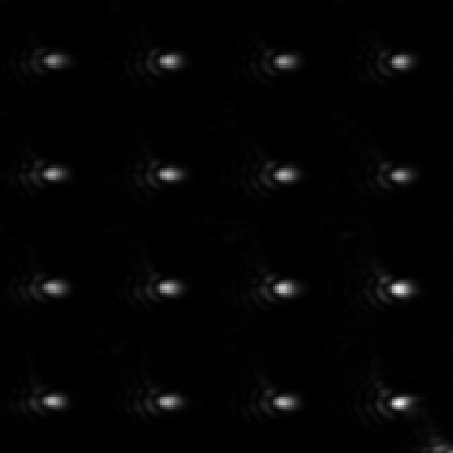
\includegraphics[width=1.4in] {grid0blue.pdf}};;
			\draw[white, fill=white] (0.65,1.1) rectangle (1.15,1.15);
			\node[color=white] at (0.73,0.8) {\footnotesize \SI{20}{\micro\meter}};
		\end{tikzpicture}
		\centering
		\caption{}
		\label{a}
	\end{subfigure}
	\begin{subfigure}[b]{.32\linewidth}
		\begin{tikzpicture}
			\centering
			\node[inner sep=0] (image) {
\includegraphics[width=1.4in] {grid1blue.pdf}};;
			
			\node[anchor=south west, color=white] at (-49pt,-45pt) {\small $5.6$};
			\node[anchor=south west, color=white] at (-23.667pt,-45pt) {\small $5.3$};
			\node[anchor=south west, color=white] at (1.333pt,-45pt) {\small $5.6$};
			\node[anchor=south west, color=white] at (27pt,-45pt) {\small $7.1$};
			
			\node[anchor=south west, color=white] at (-49pt, -20pt) {\small $5.3$};
			\node[anchor=south west, color=white] at (-23.667pt, -20pt) {\small $5.5$};
			\node[anchor=south west, color=white] at (1.333pt, -20pt) {\small $6.2$};
			\node[anchor=south west, color=white] at (27pt, -20pt) {\small $7.5$};
			
			\node[anchor=south west, color=white] at (-49pt, 5pt) {\small $5.0$};
			\node[anchor=south west, color=white] at (-23.667pt, 5pt) {\small $5.5$};
			\node[anchor=south west, color=white] at (1.333pt, 5pt) {\small $5.5$};
			\node[anchor=south west, color=white] at (27pt, 5pt) {\small $4.7$};
			
			\node[anchor=south west, color=white] at (-49pt, 30pt) {\small $4.2$};
			\node[anchor=south west, color=white] at (-23.667pt, 30pt) {\small $5.1$};
			\node[anchor=south west, color=white] at (1.333pt, 30pt) {\small $4.4$};
			\node[anchor=south west, color=white] at (27pt, 30pt) {\small $4.9$};
			
			
		\end{tikzpicture}
		\centering
		\caption{}
		\label{b}
	\end{subfigure}
	\begin{subfigure}[b]{.32\linewidth}
		\begin{tikzpicture}
			\centering
			\node[inner sep=0] (image) {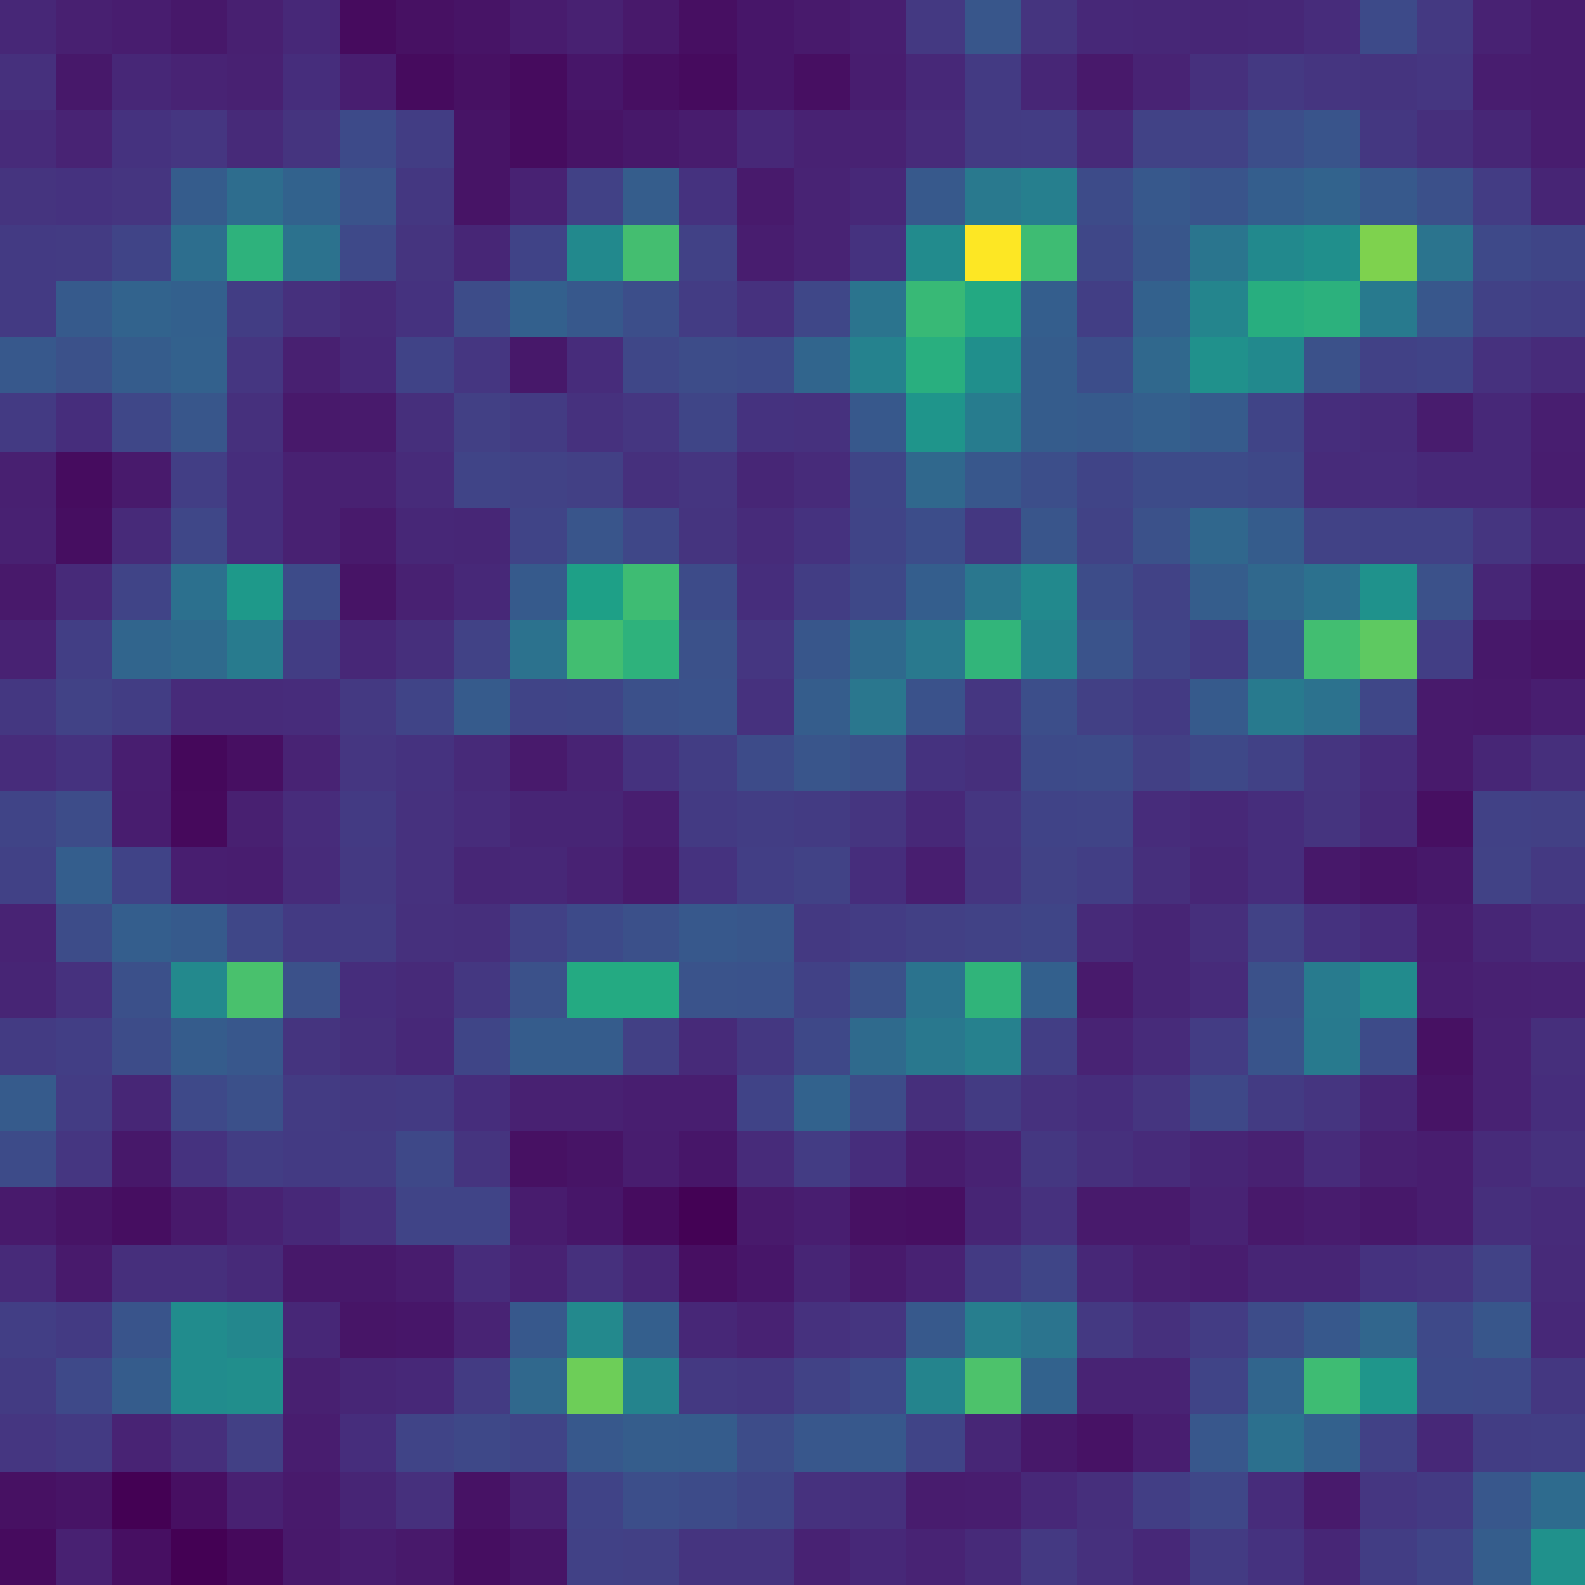
\includegraphics[width=1.4in] {grid2blue.pdf}};;
			\draw[white, fill=white] (0.65,1.1) rectangle (1.15,1.15);
			\node[color=white] at (0.73,0.8) {\small $20\,\mu$m};
		\end{tikzpicture}
		\centering
		\caption{}
		\label{c}
	\end{subfigure}
	\caption{(a) Recorded light intensity in the trapping plane. (b) Corresponding grid of optical power per trap in \si{\milli\watt}. (c) Integrated atom fluorescence. The box marks the 5 traps used for analysis of the ac-Stark shift (see \autoref{stark}). The $1/\mathrm{e}^2$ diameter of the traps is $2.2\,\mu$m.}
\end{figure}



\section{Fluorescence data processing and error analysis}

\subsection{Estimating lifetime under resonant illumination}

first discuss hysteresis method then show hann windows finally discuss

\begin{figure}[!t]
	%\vspace{0.7em}
	\centering
	\begin{tikzpicture}
		\begin{groupplot}[group style={group size=2 by 1, horizontal sep=2.5cm},height=5.5cm,width=5.5cm,no markers]
			\nextgroupplot
			[
			%title={Temperature dependence of CuSO$_4\cdot$5H$_2$O solubility},
			xlabel={Time (s)},
			ylabel={Fluorescence counts (MHz)},
			xmin=0, xmax=200,
			ymin=-0.1, ymax=0.3,
			%xtick={0,0.5,1,1.5,2},
			%xtick={0,0.5,1,1.5,2},
			%legend pos=north west,
			ymajorgrids=true,
			xmajorgrids=true,
			grid style=dashed,
			]
			
			\addplot[
			color=markrood,
			/pgfplots/error bars/.cd,
			x dir = both,
			x explicit,
			] table [col sep = comma, x index = 0, y expr=\thisrowno{1}*1.3062923961932331/0.100/1000/1000]{expgaussiansforparam_rawdata_trace.csv};
			
			\addplot[color=rainbow1of8, thick, name path=bottom] coordinates {(0,0)(200,0)};
			\addplot+[draw=none,name path=bottomb, domain=0:200, mark=none] {-0.1}; 
			\addplot+[gray, fill=rainbow1of8!80] fill between[of=bottom and bottomb,soft clip={domain=0:200}];
			
			\addplot[color=rainbow2of8, thick, name path=top] coordinates {(0,0.1)(200,0.1)};
			\addplot+[draw=none,name path=topt, domain=0:200, mark=none] {0.3}; 
			\addplot+[gray, fill=rainbow2of8!80] fill between[of=topt and top,soft clip={domain=0:200}];
			
			\nextgroupplot
			[
			ylabel=Occurrence,
			xlabel=Fluorescence counts (MHz),
			axis on top,
			enlargelimits=false
			]
			
			\addplot[
			const plot, no marks,
			draw=markrood,
			color=markrood,
			opacity=0.35
			] table [col sep = comma, x expr=\thisrowno{0}*1.3062923961932331/0.100/1000/1000, y index = 1]{expgaussiansforparam_rawdata.csv};
			
			\addplot[
			color=rainbow1of8, thick, name path=blue
			] table [col sep = comma, x expr=\thisrowno{0}*1.3062923961932331/0.100/1000/1000, y index = 1]{expgaussiansforparam.csv};
			
			%\addplot+[draw=none,name path=C, domain=4950*1.3062923961932331/0.1/1e6:0.2, mark=none] {0}; 
			%\addplot+[gray, fill=rainbow1of8!80] fill between[of=blue and C,soft clip={domain=4950*1.3062923961932331/0.1/1e6:0.2}];
			
			\addplot[
			color=rainbow2of8, thick, name path=orange
			] table [col sep = comma, x expr=\thisrowno{0}*1.3062923961932331/0.100/1000/1000, y index = 2]{expgaussiansforparam.csv};
			
			\addplot[
			color=rainbow3of8, thick, name path=green
			] table [col sep = comma, x expr=\thisrowno{0}*1.3062923961932331/0.100/1000/1000, y index = 3]{expgaussiansforparam.csv};
			
			\addplot+[draw=none,name path=D, domain=-0.1:0, mark=none] {0}; 
			\addplot+[gray, fill=rainbow1of8!80] fill between[of=blue and D,soft clip={domain=-0.1:0}];
			
			\addplot+[draw=none,name path=E, domain=0.1:0.3, mark=none] {0}; 
			\addplot+[gray, fill=rainbow2of8!80] fill between[of=orange and E,soft clip={domain=0.1:0.3}];
			
			\addplot[color=markrood, dashed] coordinates {(0,0)(0,1.2e-4)};
			\addplot[color=markrood, dashed] coordinates {(0.1,0)(0.1,1.2e-4)};
			\node[align=left, color=markrood] at (axis cs: 15500*1.3062923961932331/0.1/1e6, 1.1e-4) {\footnotesize thresholds};
			
		\end{groupplot}
		
	\end{tikzpicture}
	\caption[An example of a floating figure]{Average trap lifetime (left) and filling fraction (right) versus dipole trap power. Error bars represent the standard error of the mean based on up to three measurements of the fluorescence count rate ($50\,000$ frames) per trapping site.} % The text in the square bracket is the caption for the list of figures while the text in the curly brackets is the figure caption
	\label{fig:LTandFR} 
\end{figure}

here, discuss the Hann windows:

\begin{figure}[!t]
	%\vspace{0.7em}
	\centering
	\begin{tikzpicture}
		
		\begin{groupplot}[group style={group size=1 by 1, vertical sep=1cm},xmin=0,ymin=0,height=5.5cm,width=13.5cm,no markers]
			\nextgroupplot
			[
			%title={Temperature dependence of CuSO$_4\cdot$5H$_2$O solubility},
			xlabel={Optical power in dipole trap (\si{\milli\watt})},
			ylabel={Average trap lifetime (s)},
			xmin=0, xmax=180,
			ymin=0, ymax=10,
			%xticklabels={,,},
			%xtick={,,},
			legend pos=north east,
			legend cell align={left},
			legend style={draw=none, at={(0.98,0.94)},anchor=north east},
			ymajorgrids=true,
			xmajorgrids=true,
			grid style=dashed,
			]
			
			\addplot[
			mark size=1pt,
			only marks,
			mark = *,
			name path=dtdatapoints,
			color=rainbow1of8,
			/pgfplots/error bars/.cd,
			y dir = both,
			y explicit,
			] table [col sep = comma, x index = 0, y index = 1]{greattrace.csv};
			
			\addplot[
			forget plot,
			skip coords between index={0}{5},
			color=rainbow1of8,
			/pgfplots/error bars/.cd,
			y dir = both,
			y explicit,
			] table [col sep = comma, x index = 0, y index = 1]{greatspline.csv};
			
			\addplot[
			forget plot,
			style={ultra thin},
			skip coords between index={0}{5},
			name path=greatspline_p,
			color=rainbow1of8,
			/pgfplots/error bars/.cd,
			y dir = both,
			y explicit,
			] table [col sep = comma, x index = 0, y index = 2]{greatspline.csv};
			
			\addplot[
			forget plot,
			style={ultra thin},
			skip coords between index={0}{5},
			name path=greatspline_m,
			color=rainbow1of8,
			/pgfplots/error bars/.cd,
			y dir = both,
			y explicit,
			] table [col sep = comma, x index = 0, y index = 3]{greatspline.csv};
			
			\addplot[forget plot, rainbow1of8, opacity=0.2] fill between[
			of = greatspline_m and greatspline_p,
			]; 
			
			
			\addplot[
			mark size=1pt,
			only marks,
			mark = *,
			skip coords between index={0}{1},
			color=rainbow2of8,
			/pgfplots/error bars/.cd,
			y dir = both,
			y explicit,
			] table [col sep = comma, x index = 0, y index = 1]{Hann400trace.csv};
			
			\addplot[
			forget plot,
			skip coords between index={0}{105},
			name path=Hann400trace,
			color=rainbow2of8,
			/pgfplots/error bars/.cd,
			y dir = both,
			y explicit,
			] table [col sep = comma, x index = 0, y index = 1]{hannseriesspline_400.csv};
			
			\addplot[
			forget plot,
			style={ultra thin},
			skip coords between index={0}{105},
			name path=Hann400trace_p,
			color=rainbow2of8,
			/pgfplots/error bars/.cd,
			y dir = both,
			y explicit,
			] table [col sep = comma, x index = 0, y index = 2]{hannseriesspline_400.csv};
			
			\addplot[
			forget plot,
			style={ultra thin},
			skip coords between index={0}{105},
			name path=Hann400trace_m,
			color=rainbow2of8,
			/pgfplots/error bars/.cd,
			y dir = both,
			y explicit,
			] table [col sep = comma, x index = 0, y index = 3]{hannseriesspline_400.csv};
			
			\addplot[forget plot, rainbow2of8, opacity=0.2] fill between[
			of = Hann400trace_m and Hann400trace_p,
			];
			
			
			\addplot[
			mark size=1pt,
			only marks,
			mark = *,
			skip coords between index={0}{1},
			color=rainbow3of8,
			/pgfplots/error bars/.cd,
			y dir = both,
			y explicit,
			] table [col sep = comma, x index = 0, y index = 1]{Hann500trace.csv};
			
			\addplot[
			forget plot,
			skip coords between index={0}{105},
			name path=Hann500trace,
			color=rainbow3of8,
			/pgfplots/error bars/.cd,
			y dir = both,
			y explicit,
			] table [col sep = comma, x index = 0, y index = 1]{hannseriesspline_500.csv};
			
			\addplot[
			forget plot,
			style={ultra thin},
			skip coords between index={0}{105},
			name path=Hann500trace_p,
			color=rainbow3of8,
			/pgfplots/error bars/.cd,
			y dir = both,
			y explicit,
			] table [col sep = comma, x index = 0, y index = 2]{hannseriesspline_500.csv};
			
			\addplot[
			forget plot,
			style={ultra thin},
			skip coords between index={0}{105},
			name path=Hann500trace_m,
			color=rainbow3of8,
			/pgfplots/error bars/.cd,
			y dir = both,
			y explicit,
			] table [col sep = comma, x index = 0, y index = 3]{hannseriesspline_500.csv};
			
			\addplot[forget plot, rainbow3of8, opacity=0.2] fill between[
			of = Hann500trace_m and Hann500trace_p,
			]; 		
			
			
			\addplot[
			mark size=1pt,
			only marks,
			mark = *,
			skip coords between index={0}{1},
			color=rainbow4of8,
			/pgfplots/error bars/.cd,
			y dir = both,
			y explicit,
			] table [col sep = comma, x index = 0, y index = 1]{Hann600trace.csv};
			
			\addplot[
			forget plot,
			skip coords between index={0}{105},
			name path=Hann600trace,
			color=rainbow4of8,
			/pgfplots/error bars/.cd,
			y dir = both,
			y explicit,
			] table [col sep = comma, x index = 0, y index = 1]{hannseriesspline_600.csv};
			
			\addplot[
			forget plot,
			style={ultra thin},
			skip coords between index={0}{105},
			name path=Hann600trace_p,
			color=rainbow4of8,
			/pgfplots/error bars/.cd,
			y dir = both,
			y explicit,
			] table [col sep = comma, x index = 0, y index = 2]{hannseriesspline_600.csv};
			
			\addplot[
			forget plot,
			style={ultra thin},
			skip coords between index={0}{105},
			name path=Hann600trace_m,
			color=rainbow4of8,
			/pgfplots/error bars/.cd,
			y dir = both,
			y explicit,
			] table [col sep = comma, x index = 0, y index = 3]{hannseriesspline_600.csv};
			
			\addplot[forget plot, rainbow4of8, opacity=0.2] fill between[
			of = Hann600trace_m and Hann600trace_p,
			]; 		
			
			
			\addplot[
			mark size=1pt,
			only marks,
			mark = *,
			skip coords between index={0}{1},
			color=rainbow5of8,
			/pgfplots/error bars/.cd,
			y dir = both,
			y explicit,
			] table [col sep = comma, x index = 0, y index = 1]{Hann700trace.csv};
			
			\addplot[
			forget plot,
			skip coords between index={0}{105},
			name path=Hann700trace,
			color=rainbow5of8,
			/pgfplots/error bars/.cd,
			y dir = both,
			y explicit,
			] table [col sep = comma, x index = 0, y index = 1]{hannseriesspline_700.csv};
			
			\addplot[
			forget plot,
			style={ultra thin},
			skip coords between index={0}{105},
			name path=Hann700trace_p,
			color=rainbow5of8,
			/pgfplots/error bars/.cd,
			y dir = both,
			y explicit,
			] table [col sep = comma, x index = 0, y index = 2]{hannseriesspline_700.csv};
			
			\addplot[
			forget plot,
			style={ultra thin},
			skip coords between index={0}{105},
			name path=Hann700trace_m,
			color=rainbow5of8,
			/pgfplots/error bars/.cd,
			y dir = both,
			y explicit,
			] table [col sep = comma, x index = 0, y index = 3]{hannseriesspline_700.csv};
			
			\addplot[forget plot, rainbow5of8, opacity=0.2] fill between[
			of = Hann700trace_m and Hann700trace_p,
			]; 	
			
			
			\addplot[
			mark size=1pt,
			only marks,
			mark = *,
			skip coords between index={0}{1},
			color=rainbow6of8,
			/pgfplots/error bars/.cd,
			y dir = both,
			y explicit,
			] table [col sep = comma, x index = 0, y index = 1]{Hann800trace.csv};
			
			\addplot[
			forget plot,
			skip coords between index={0}{105},
			name path=Hann800trace,
			color=rainbow6of8,
			/pgfplots/error bars/.cd,
			y dir = both,
			y explicit,
			] table [col sep = comma, x index = 0, y index = 1]{hannseriesspline_800.csv};
			
			\addplot[
			forget plot,
			style={ultra thin},
			skip coords between index={0}{105},
			name path=Hann800trace_p,
			color=rainbow6of8,
			/pgfplots/error bars/.cd,
			y dir = both,
			y explicit,
			] table [col sep = comma, x index = 0, y index = 2]{hannseriesspline_800.csv};
			
			\addplot[
			forget plot,
			style={ultra thin},
			skip coords between index={0}{105},
			name path=Hann800trace_m,
			color=rainbow6of8,
			/pgfplots/error bars/.cd,
			y dir = both,
			y explicit,
			] table [col sep = comma, x index = 0, y index = 3]{hannseriesspline_800.csv};
			
			\addplot[forget plot, rainbow6of8, opacity=0.2] fill between[
			of = Hann800trace_m and Hann800trace_p,
			];
			
			
			\addplot[
			mark size=1pt,
			only marks,
			mark = *,
			skip coords between index={0}{1},
			color=rainbow7of8,
			/pgfplots/error bars/.cd,
			y dir = both,
			y explicit,
			] table [col sep = comma, x index = 0, y index = 1]{Hysttrace.csv};
			
			\addplot[
			forget plot,
			skip coords between index={0}{5},
			name path=Hysttrace_p,
			color=rainbow7of8,
			/pgfplots/error bars/.cd,
			y dir = both,
			y explicit,
			] table [col sep = comma, x index = 0, y index = 1]{Hystspline.csv};
			
			\addplot[
			forget plot,
			style={ultra thin},
			skip coords between index={0}{5},
			name path=Hysttrace_p,
			color=rainbow7of8,
			/pgfplots/error bars/.cd,
			y dir = both,
			y explicit,
			] table [col sep = comma, x index = 0, y index = 2]{Hystspline.csv};
			
			\addplot[
			forget plot,
			style={ultra thin},
			skip coords between index={0}{5},
			name path=Hysttrace_m,
			color=rainbow7of8,
			/pgfplots/error bars/.cd,
			y dir = both,
			y explicit,
			] table [col sep = comma, x index = 0, y index = 3]{Hystspline.csv};
			
			\addplot[forget plot, rainbow7of8, opacity=0.2] fill between[
			of = Hysttrace_m and Hysttrace_p,
			]; 		
			
			\addlegendentry{\footnotesize \hspace{0.5em}No filter}
			\addlegendentry{\footnotesize \hspace{0.5em}\SI{400}{\ms}}
			\addlegendentry{\footnotesize \hspace{0.5em}\SI{500}{\ms}}
			\addlegendentry{\footnotesize \hspace{0.5em}\SI{600}{\ms}}
			\addlegendentry{\footnotesize \hspace{0.5em}\SI{700}{\ms}}
			\addlegendentry{\footnotesize \hspace{0.5em}\SI{800}{\ms}}
			\addlegendentry{\footnotesize \hspace{0.5em}Hysteresis}
				
		\end{groupplot}
		
	\end{tikzpicture}
	\caption[An example of a floating figure]{Average trap lifetime (left) and filling fraction (right) versus dipole trap power. Error bars represent the standard error of the mean based on up to three measurements of the fluorescence count rate ($50\,000$ frames) per trapping site.} % The text in the square bracket is the caption for the list of figures while the text in the curly brackets is the figure caption
	\label{fig:LTandFR} 
\end{figure}


how to combine datasets appendix formulas and sample sizes:

\begin{figure}[!t]
	%\vspace{0.7em}
	\centering
	\begin{tikzpicture}
		\begin{groupplot}[group style={group size=1 by 1, vertical sep=1cm},xmin=0,ymin=0,height=5.5cm,width=13.5cm,no markers]
			\nextgroupplot
			[
			%title={Temperature dependence of CuSO$_4\cdot$5H$_2$O solubility},
			xlabel={Optical power in dipole trap (\si{\milli\watt})},
			ylabel={Lifetime sample size},
			xmin=0, xmax=180,
			ymin=0, ymax=600,
			%xtick={0,0.5,1,1.5,2},
			%xtick={0,0.5,1,1.5,2},
			%legend pos=north west,
			ymajorgrids=true,
			xmajorgrids=true,
			grid style=dashed,
			]
			
			\addplot[
			only marks,
			mark = *,
			color=markrood,
			/pgfplots/error bars/.cd,
			x dir = both,
			x explicit,
			] table [col sep = comma, x index = 0, y index = 1, x error expr=\thisrowno{2}]{samplesizesforerroranalysis.csv};
			
			\iffalse
			\addplot[
			color=markrood,
			/pgfplots/error bars/.cd,
			y dir = both,
			y explicit,
			] table [col sep = comma, x index = 0, y index = 1]{darktimecalibrationfit.csv};
			\fi
			%\node[font=\small, color=markrood] at (axis cs: 1.2, 0.2) {$y=0.137 + x$};
		\end{groupplot}
		
	\end{tikzpicture}
	\caption[An example of a floating figure]{Average trap lifetime (left) and filling fraction (right) versus dipole trap power. Error bars represent the standard error of the mean based on up to three measurements of the fluorescence count rate ($50\,000$ frames) per trapping site.} % The text in the square bracket is the caption for the list of figures while the text in the curly brackets is the figure caption
	\label{fig:LTandFR} 
\end{figure}



\subsection{Estimating dark lifetime}
then discuss alpha stuff then 

% Set the overall layout of the tree
\tikzstyle{level 1}=[level distance=3.5cm, sibling distance=2.4cm]
\tikzstyle{level 2}=[level distance=3.5cm, sibling distance=3cm]
\tikzstyle{level 3}=[level distance=3.5cm, sibling distance=1.5cm]


% Define styles for bags and leafs
\tikzstyle{bag} = [text width=4em, text centered, font=\small]
\tikzstyle{end} = [circle, minimum width=3pt,fill, inner sep=0pt]

\begin{figure}
\begin{tikzpicture}[grow=right, sloped]

	\node[bag] (Root) {No}
	child {
		node[bag] {No,\\terminate}
		edge from parent 
		node[above] {\tiny correct}
		node[below]  {$p$}
	}
	child {
		node[bag] (Root1) {Yes,\\wait $\Delta t$}        
		child {
			node[bag] (Root2) {No}
			child {
				node[bag] {No}
				edge from parent
				node[above] {}
				node[below, font=\small]  {$p$}
			}
			child {
				node[bag] (Root3) {Yes}
				edge from parent
				node[above] {}
				node[below, font=\small]  {$1-p$}
			}
			edge from parent
			node[above] {}
			node[below, font=\small]  {$1$}
		}
		edge from parent         
		node[above] {\tiny type I error}
		node[below, font=\small]  {$1-p$}
	};
	
	\node[bag, below= 4cm of Root] {Yes}
	child {
		node[bag] {No,\\terminate}        
		edge from parent 
		node[above] {\tiny type II error}
		node[below, font=\small]  {$1-p$}
	}
	child {
		node[bag] {Yes, wait $\Delta t$}        
		child {
			node[bag] {No}
			child {
				node[bag] {No}
				edge from parent
				node[above] {}
				node[below, font=\small]  {$p$}
			}
			child {
				node[bag] {Yes}
				edge from parent
				node[above] {}
				node[below, font=\small]  {$1-p$}
			}
			edge from parent
			node[above] {}
			node[below, font=\small]  {$1-P$}
		}
		child {
			node[bag] {Yes}
			child {
				node[bag] {No}
				edge from parent
				node[above] {}
				node[below, font=\small]  {$1-p$}
			}
			child {
				node[bag] {Yes}
				edge from parent
				node[above] {}
				node[below, font=\small]  {$p$}
			}
			edge from parent
			node[above] {}
			node[below, font=\small]  {$P$}
		}
		edge from parent         
		node[above] {\tiny correct}
		node[below, font=\small]  {$p$}
	};
	
	
	\begin{scope}[every node/.style={text width=3cm, align=center, anchor=center, font=\small}]
		\node[above= 0.5cm of Root3] (labels-level) {Measurement 2: Atom detected?};
		\node[at =(labels-level-|Root2)] {Reality:\\ Atom survived?};
		\node[at =(labels-level-|Root1)] {Measurement 1: Atom detected?};
		\node[at =(labels-level-|Root)] {Reality:\\ Atom present?};
		
	\end{scope}
	
\end{tikzpicture}
	\caption[An example of a floating figure]{asdlfk sdfoiwe foijwe oifj weoifrj slkdjf 9wiejf oweijfwsljfr we9oijfwloeijf woeijf woejf woedijf weoifjmw eoifrj woeifj woefjw eoifj weoifj weojf } % The text in the square bracket is the caption for the list of figures while the text in the curly brackets is the figure caption
\label{fig:LTandFR} 
\end{figure}




\begin{figure}
\centering
\begin{tikzpicture}
	\begin{groupplot}[group style={group size=2 by 2, horizontal sep=2.5cm, vertical sep=2.5cm }, height=5.5cm, width=5.5cm, no markers]
	
	\nextgroupplot
	[
	no markers,
	domain=0:10,
	y domain=0:0.5,
	ymin=0,
	ymax=0.5,
	samples=100,
	axis lines*=left,
	ylabel=Occurrence,
	xlabel=Fluorescence counts,
	%every axis y label/.style={at=(current axis.above origin),anchor=south},
	%every axis x label/.style={at=(current axis.right of origin),anchor=west},
	ytick={0.5},
	yticklabels={},	
	xtick={4,6},
	xticklabels={$\mu_1$, $\mu_2$},
	%ytick=\empty,
	enlargelimits=false,
	clip=false,
	axis on top,
	]
	
	\addplot [fill=rainbow1of8!20, draw=none, domain=0:5] {gauss(4,1)} \closedcycle;
	\addplot [fill=rainbow2of8!20, draw=none, domain=5:10] {gauss(6,1)} \closedcycle;
	\addplot [fill=rainbow2of8!80, draw=none, domain=0:5] {gauss(6,1)} \closedcycle;
	\addplot [fill=rainbow1of8!80, draw=none, domain=5:10] {gauss(4,1)} \closedcycle;
	\addplot [rainbow1of8, thick] {gauss(4,1)};
	\addplot [rainbow2of8, thick] {gauss(6,1)};
	
	\addplot[color=markrood, dashed] coordinates {(5,0)(5,0.5)};
	\node[align=left, color=markrood] at (2.5,0.45) {\footnotesize threshold};
	
	\node[align=left, color=rainbow2of8] at (6,0.25) {\footnotesize $p$};
	\node[align=left, color=rainbow2of8] at (2.7,0.15) {\footnotesize $1-p$};
	
	\node[align=left, color=rainbow1of8] at (4,0.25) {\footnotesize $p$};
	\node[align=left, color=rainbow1of8] at (7.3,0.15) {\footnotesize $1-p$};		
	
	\addplot[color=rainbow2of8] coordinates {(4,0.05)(2.7,0.12)};
	\addplot[color=rainbow1of8] coordinates {(6,0.05)(7.3,0.12)};
	
	\nextgroupplot
	[
	ylabel=Occurrence,
	xlabel=Fluorescence counts (MHz),
	axis on top,
	enlargelimits=false
	]
	
	\addplot[
	const plot, no marks,
	draw=markrood,
	color=markrood,
	opacity=0.35
	] table [col sep = comma, x expr=\thisrowno{0}*1.3062923961932331/0.100/1000/1000, y index = 1]{expgaussiansforparam_rawdata.csv};
	
	\addplot[
	color=rainbow1of8, thick, name path=blue
	] table [col sep = comma, x expr=\thisrowno{0}*1.3062923961932331/0.100/1000/1000, y index = 1]{expgaussiansforparam.csv};
	
	\addplot+[draw=none,name path=C, domain=4950*1.3062923961932331/0.1/1e6:0.2, mark=none] {0}; 
	\addplot+[gray, fill=rainbow1of8!80] fill between[of=blue and C,soft clip={domain=4950*1.3062923961932331/0.1/1e6:0.2}];
	
	\addplot[
	color=rainbow2of8, thick, name path=orange
	] table [col sep = comma, x expr=\thisrowno{0}*1.3062923961932331/0.100/1000/1000, y index = 2]{expgaussiansforparam.csv};
	
	\addplot[
	color=rainbow3of8, thick
	] table [col sep = comma, x expr=\thisrowno{0}*1.3062923961932331/0.100/1000/1000, y index = 3]{expgaussiansforparam.csv};
	
	\addplot+[draw=none,name path=B, domain=-0.1:4950*1.3062923961932331/0.1/1e6, mark=none] {0}; 
	\addplot+[gray, fill=rainbow2of8!80] fill between[of=orange and B,soft clip={domain=-0.1:4950*1.3062923961932331/0.1/1e6}];
	
	\addplot[color=markrood, dashed] coordinates {(4950*1.3062923961932331/0.1/1e6,0)(4950*1.3062923961932331/0.1/1e6,1.2e-4)};
	\node[align=left, color=markrood] at (axis cs: 12500*1.3062923961932331/0.1/1e6, 1.1e-4) {\footnotesize threshold};
	
	\node[align=left, color=rainbow1of8] at (0.135,0.1e-4) {\footnotesize \SI{1}{\percent}};
	
	\node[align=left, color=rainbow2of8] at (0,0.1e-4) {\footnotesize \SI{4}{\percent}};
	

	

	
	\nextgroupplot
	[
	view={-60}{30},
	colormap/viridis,
	xlabel={$P$},
	ylabel={$p$},
	zlabel={$P_\text{d}$},
	]
	
	\addplot3 [
	surf,
	domain=0:1,
	y domain=0.5:1,
	samples=20,
	] {x*(2*y^2 - y) + 1 - y};
	
	\nextgroupplot
	[
	axis on top,
	xlabel={$P$},
	ylabel={$P_\text{d}$},
	enlargelimits=false
	]
	
	\plot[name path=f26,thick,opacity=0,samples=100,domain=0:1] {x*(0.75^2*2-0.75)+1-0.75};
	\plot[name path=f25,thick,opacity=0,samples=100,domain=0:1] {0.4};
	\plot[name path=f24,thick,opacity=0,samples=100,domain=0:1] {0.325};
	
	\addplot fill between[
	of = f25 and f24,
	soft clip={domain=0:0.2},
	every even segment/.style  = {rainbow3of8!20}
	];
	
	\addplot fill between[
	of = f26 and f25,
	soft clip={domain=0.2:0.4},
	every even segment/.style  = {rainbow3of8!20}
	];
	
	\addplot [fill=rainbow3of8!20, draw=none, domain=0.2:0.4] {x*(0.75^2*2-0.75)+1-0.75} \closedcycle;
	
	\addplot [
	domain=0:1,
	y domain=0:1,
	samples=100,
	color=rainbow1of8
	] {x};
	
	\node[align=left, color=rainbow1of8, rotate=45] at (0.75,0.83) {\footnotesize $p=1$};
	
	\addplot [
	domain=0:1,
	y domain=0:1,
	samples=100,
	color=rainbow2of8
	] {0.5};
	
	\node[align=left, color=rainbow2of8] at (0.2,0.555) {\footnotesize $p=0.5$};
	
	\addplot [
	domain=0:1,
	y domain=0:1,
	samples=100,
	color=rainbow3of8
	] {x*(0.75^2*2-0.75)+1-0.75};
	
	\node[align=left, color=rainbow3of8, rotate=20.5560452] at (0.8,0.612) {\footnotesize $p=0.75$};
	
	\addplot [
	domain=0:0.2,
	y domain=0:1,
	samples=100,
	dashed,
	color=rainbow3of8
	] {0.325};
	
	\addplot [
	domain=0:0.63,
	y domain=0:1,
	samples=100,
	dashed,
	color=rainbow3of8
	] {0.4};
	
	\addplot [
	domain=0:0.63,
	y domain=0:1,
	samples=100,
	dashed,
	color=rainbow3of8
	] {0.3625};
	
	\draw[color=rainbow3of8, dashed] 
	(axis cs:0.2, 0) -- (axis cs:0.2, 0.325);
	
	\draw[color=rainbow3of8, dashed] 
	(axis cs:0.3, 0) -- (axis cs:0.3, 0.3625);
	
	\draw[color=rainbow3of8, dashed] 
	(axis cs:0.4, 0) -- (axis cs:0.4, 0.4);
	
	\node[align=left, color=rainbow3of8] at (0.79,0.38) {\footnotesize $\Delta P_\text{d}$};
	\node[align=left, color=rainbow3of8] at (0.53,0.2) {\footnotesize $\Delta P$};
	
	\draw[<->, rainbow3of8] (0.3,0.2) to (0.4, 0.2);
	\draw[->, rainbow3of8] (0.65,0.3025) to (0.65, 0.3625);
	\draw[->, rainbow3of8] (0.65,0.46) to (0.65, 0.4);
	
	
	\end{groupplot}
\end{tikzpicture}
	\caption[An example of a floating figure]{detected survival probability $P_d$ as a function of Distinguishability $p$ and atom survival probability $P$} % The text in the square bracket is the caption for the list of figures while the text in the curly brackets is the figure caption
\label{fig:LTandFR} 
\end{figure}

Probability of detecting a survival $P_\text{d}$, i.e. atom in measurement 1 and atom in measurement 2, in terms of actual survival probability $P$).
\begin{equation}
	P_\text{d}=  (1-p)^2 + p\left(Pp + (1-P)(1-p) \right)
\end{equation}
which can be inverted to find
\begin{equation}
	P = \frac{P_\text{d}}{2p^2-p} + \frac{p-1}{2p^2-p}
\end{equation}
limit $p\rightarrow 1$ gives $P\rightarrow P_d$ and worst case scenario $p\rightarrow 0.5$ gives $P\rightarrow \infty$, which also means infinity errors.
\begin{equation}
	\Delta P = \Delta P_\text{d} \left| \diff{P}{P_\text{d}} \right|=\frac{1}{2p^2-p},\hspace{1em} p > 0.5
\end{equation}

\subsection{Trap depth correction through ac-Stark shift}

\iffalse
\begin{figure}[tb]
	\centering
	\includegraphics[width=0.8\textwidth]{summary.pdf}
	\caption{}
	\label{fig:singleAtomGraph}
\end{figure}

\begin{figure}[tb]
	\centering
	\includegraphics[width=1\textwidth]{multifit.pdf}
	\caption{}
	\label{fig:singleAtomGraph}
\end{figure}

\begin{figure}[tb]
	\centering
	\includegraphics[width=0.8\textwidth]{correctedLT.pdf}
	\caption{}
	\label{fig:singleAtomGraph}
\end{figure}

\begin{figure}[tb]
	\centering
	\includegraphics[width=0.8\textwidth]{correctedFR.pdf}
	\caption{}
	\label{fig:singleAtomGraph}
\end{figure}
\fi

\section{Conclusion}
We find that we are able to create single-atom dipole traps with a loading rate of \SI{0.32}{\per\second} using a shallow depth of \SI{442}{\mega\hertz}, and a lifetime of \SI{8.2}{\second} using a deeper depth of \SI{833}{\mega\hertz}. We also see that we are able to switch from a shallow trap to a deep one with \SI{98}{\percent} success in keeping the atom trapped in the process, demonstrating that increasing the depth of the trap does not disturb the atom significantly. 






% - by this point will have defined the experimental setup fully and we're at the stage where we the reader knows we have a 1 micron (well 1.6 micron with M^2 factor) trap within a MOT. 
% - have also made reference to the SLM and therefore know we have multiple identical traps (but that this isn't a big deal like, it just means faster data collection). 
% - also have discussed what parameters will have an effect on trap behaviour (namely - trap depth and MOT detuning are the easily experimentally controllable things that will have an obvious effect... and they are closely linked)
% - all of the parameters we actually use will have been detailed in the experimental setup section too (i.e. vacuum pressure, mot powers, trap size, mot detuning; will have also explained that we put a small sinusoidal oscillation on the MOT frequency to wash out interference fringes and give a more reliably constant local MOT density)
\iffalse
We systematically investigate the effects of the depth of the dipole-force trap on the average lifetime, loading rate and filling ratio of the trap. We vary the power per trap between \SI{18.5}{\milli\watt} and \SI{124.0}{\milli\watt} by changing the voltage sent to the AOM in the trapping light beam path. These powers were chosen as the minimum power at which we observe the traps ever being occupied and the maximum power at which single occupation of the trap can be reliably observed.

%\subsection{Methods}

For each chosen depth, we use the single-atom imaging camera to register the fluorescence emitted from all traps for $20$ minutes with a time resolution of \SI{250}{\ms}. In combination with a high EM gain of $800$, this allows us to clearly distinguish when there is an atom in a trap. Even for deep traps, where the large Stark shifts reduce the fluorescence rate drastically\footnote{We note that at these kinds of Stark shifts we wouldn't actually expect the cooling to work or to observe any significant fluorescence; we will come back to this in (reference ahead to the the modelling section)}, the signal-to-noise ratio is excellent. This process is carried out with the MOT running, so that we may observe fluorescence light.

\fi

%We take an acquisition using the single-atom imaging camera for each of the trap depths that we use; in each case the acquisition is \num{5000} frames long and each frame has an exposure time of \SI{250}{\ms} (i.e. approximately a \num{20} minute acquisition in total). This long exposure time is necessary, as is a high EM gain of \num{800}, in order to get a good enough signal-to-noise ratio to clearly distinguish when there is an atom in a trap. This is particularly the case for deep traps where we also have greater Stark shifts and hence less fluorescence from the trapped atoms\footnote{We note that at these kinds of Stark shifts we wouldn't actually expect the cooling to work or to observe any significant fluorescence; we will come back to this in (reference ahead to the the modelling section)}, making for a weaker signal. At the trapping light powers we use, enough scattered light gets through the \SI{780}{\nm} bandpass filter in front of the camera that we have a significant amount of background noise.

\iffalse
\begin{figure}[tb]
	\centering
	\includegraphics[width=\textwidth]{singleAtomGraph_example.pdf}
	\caption{A typical graph of observed fluorescence as a function of time for a single-atom dipole trap. The graph shows two distinct levels, corresponding to an empty trap (lower level) and a trap occupied by a single atom (upper level).}
	\label{fig:singleAtomGraph}
\end{figure}



From the fluorescence data for each of the trapping sites we calculate an average lifetime, filling ratio, and loading rate for each combination of the parameters. An example single-atom fluorescence trace is shown in \cref{fig:singleAtomGraph}. We see that a single-atom trap exhibits two distinct levels of fluorescence. We say that a trap is occupied when its fluorescence exceeds a threshold value that is defined as half-way between the average lower level fluorescence and the average upper level fluorescence. The filling ratio of a trap is the fraction of the time that it is occupied, i.e. the percentage of data points in the trace that are above the threshold. To determine the lifetime we find, for each trap, every instance that it is occupied and measure the length of time it is occupied for. We bin the data to form a histogram and fit an exponential decay function from which we extract the average lifetime. We do the same with the sections for which the trap is empty to determine the average loading time, from which we obtain the loading rate as the reciprocal. We note that in the limit that light-assisted collisions totally dominate loss from the trap, the filling ratio tends to \num{0.5} and thus the average loading time and the average lifetime will be the same. 



%\subsection{Results}

The results of varying the trap depth are shown in \cref{table:depthSweep}. 

\begin{table}[]
	\centering
	%\vspace{5mm}
	\begin{tabular}{llllll} \toprule
		Power (\si{\milli\watt}}{unit commands}) & Depth (\si{\mega\hertz}) & Lifetime (\si{\second}) & filling ratio & Load Rate (\si{\per\second}) \\ \midrule
		18.5 & 160 & \num{0.3 \pm 0.2} & \num{0.02 \pm 0.01} & \num{0.07 \pm 0.003} \\ 
		34.1 & 293 & \num{3.4 \pm 0.3} & \num{0.46 \pm 0.01} & \num{0.22 \pm 0.006} \\ 
		51.3 & 442 & \num{6.6 \pm 0.4} & \num{0.49 \pm 0.02} & \num{0.15 \pm 0.006} \\ 
		66.6 & 573 & \num{7.8 \pm 0.4} & \num{0.47 \pm 0.02} & \num{0.11 \pm 0.007} \\ 
		81.0 & 697 & \num{9.8 \pm 0.5} & \num{0.43 \pm 0.02} & \num{0.08 \pm 0.007} \\ 
		96.8 & 833 & \num{10.1 \pm 0.4} & \num{0.40 \pm 0.02} & \num{0.07 \pm 0.006} \\ 
		109.8 & 945 & \num{9.5 \pm 0.4} & \num{0.39 \pm 0.02} & \num{0.07 \pm 0.008} \\ 
		124.0 & 1069 & \num{9.8 \pm 0.5} & \num{0.36 \pm 0.02} & \num{0.06 \pm 0.006}  \\ \bottomrule
	\end{tabular} \\
	\caption{Results of varying the power per dipole trap, for \num{10} trapping sites that are identical up to the limits outlined in (REF the experimental setup section). The errors on the lifetime and loading rate are taken from the \SI{90}{\percent} confidence intervals of the exponential fits, while the error on the filling ratio is the standard deviation between the values observed at each of the \num{10} trapping sites.}
	\label{table:depthSweep}
\end{table}

\begin{figure}[tb]
	\centering
	\includegraphics[width=\textwidth]{gridData.pdf}
	\caption{Measured average lifetime, loading rate and filling ratio as a function of trap power.}
	\label{fig:gridData}
\end{figure}

In \cref{fig:gridData} we plot the lifetime, loading rate and filling ratio as a function of trap power. We see that the lifetime increases as we put more power into the trap to make it deeper. Meanwhile after an initial rise, corresponding to the trap power reaching the required threshold to successfully trap an atom, we see the filling ratio and loading rate both drop as the power increases.

Qualitatively speaking, we would expect shallower traps to capture atoms more readily - the Stark shift is lower and hence the MOT cooling is more effective, so a greater proportion of the surrounding atoms may be trapped. Meanwhile, it also makes sense that deeper traps would generally keep an atom held for longer, since only the colder atoms will be capable of being trapped in the first place and we would expect colder atoms to remain trapped for longer on average.


\section{Getting the best of both worlds}

We have seen that a shallower trap gives us a faster loading rate, while a deeper trap gives a longer lifetime. This result implies that one can use a fast-loading trap of shallow depth at first, and a deep trap of long lifetime once and atom is trapped. This would require starting out with a shallow trap and increasing the depth at the very moment that an atom enters it.

We demonstrate this concept without actually implementing such an active feedback based upon the presence of an atom; rather, we switch the trap depth at fixed points in time using the AOM in the trapping light beam path and post-select on atoms that were present when the switch from a shallow trap to a deep trap is made. For each such atom we may then trace backwards in time to see at what point that atom entered the shallow trap, and forwards in time to see how long the atom remained in the deep trap.
\fi




Based on these results, we choose a loading depth of $d_\mathrm{l} = \SI{442}{\mega\hertz}$ (i.e. a power per trap of \SI{34.1}{\milli\watt}) and a holding depth of $d_\mathrm{h} = \SI{833}{\mega\hertz}$ (i.e. a power per trap of \SI{96.8}{\milli\watt}).






\subsection{Methods}
\label{subsec:switchMethod}









\iffalse
The result of stacking up the fluorescence traces for atoms present when the trap depth is increased, as described in \cref{subsec:switchMethod}, is displayed in \cref{fig:switchData}b. We have separately normalised the average fluorescence for a single atom to \num{1} for each of the two regimes. We find \num{623} instances where an atom was present at the time that the switch was made; this is in line with our expectation that we would see approximately \num{600} such occurrences. The data here is presented in units of counts per second and per trap (i.e. after stacking up normalised fluorescence traces we divide by \num{623} - the number of fluorescence traces making up the graph). We see an exponential decay either side of $t=0$. We plot the same data with a log-linear scale in \cite{fig:switchData}c. From the gradient $d\ln(\mathrm{count\,\,rate})/dt$ we extract average lifetimes for a shallow and a deep trap as \SI{3.1\pm0.1}{\s} and \SI{8.2\pm0.3}{\s} respectively. 

For the shallow depth we measure an average filling ratio (across all \num{10} sites at all periods of low power) of \num{0.48}. The fact that this is so close to \num{0.5} means we can take the lifetime to be equivalent to the loading time. This gives us a loading rate of $1/3.1 = \SI{0.32}{\per\second}$ for the shallow trap. We have thus demonstrated that we can load atoms fast by using shallow traps, then keep these atoms trapped for longer by increasing the depth of the traps. 

One important question remains: with what success do we keep the atom trapped while increasing the depth? In other words, do we ever lose the trapped atom as a result of changing the depth of the trap? We see in \cite{fig:switchData}a two instances at which the atom remains trapped while the depth is increased since the background-corrected fluorescence drops immediately to the new value for an occupied deep trap rather than falling to zero (we also see one instance where the trap is empty at the moment in time that the switch is made). But are we always this successful? We have this information in \cite{fig:switchData}b. The height of the left-hand exponential, i.e. the data for before the depth is increased, is \num{1} by definition of how the data is selected. The height of the right-hand exponential at $t=0$ tells us what fraction of the atoms are still trapped the instant after the depth is increased. We find that we successfully keep $98\%$ of the atoms.



\fi
%
%
%% 1. behaviour as a function of depth
%% 2. methods for collecting depth change data
%% 3. results of depth change data
%
%(maybe this needs a better name...? basically a section of how we do all the pre-requisite shit for the cool stuff to work)
%
%\begin{itemize}
%  \item we generate holograms using an adaptive  algorithm which enables us to get grids of trap with high uniformity.. ie all the same depth (quote the coefficient of variation)
%  \item we scan MOT detunings and trap powers to identify different regimes (fast loading vs long lifetime) ... i have graphs that can be included here
%  \item we use a DAQ card to send triggers to change the total power via an AOM every 30 seconds to switch between these regimes and post-select on atoms that were present at the time a switch was made from shallow (fast loading) to deep (long lifetime) 
%  \item include enough description of the post-selection process and how we count backwards/forwards until atom is lost, plus equivalence of lifetime and inverse of loading rate based on filling ratio of approx 50\%, to be convincing
%  \item mention the process of normalising the fluorescence because the fluorescence detected is different in each regime due to the differing stark shifts 
%  \item anything else key about our process that i've missed here?
%\end{itemize}
% 
%\section{Results}
% 
%\begin{itemize}
%  \item present the graphs from my thesis showing that we basically lose no atoms in the process of switching (98\% success) and that we have exponential decays with different timescales in the shallow vs deep regime
%  \item quote the lifetimes in each regime and calculate an effective obtainable filling ratio (72\%) if we were able to use this concept to selectively deepen a trap when an atom enters it
%\end{itemize}
% 



\subsection{Dynamic holograms for moving atoms}
\label{exp3}
Once it is possible to fill holographic static microtraps located inside the optical cavity (\autoref{exp4} and \autoref{exp5}), dynamic holograms are necessary to enable selective positioning of single atoms in the optical field mode. The main problem is caused by intensity fluctuations in the trapping potential which are the result of sudden phase changes of a liquid crystal SLM \cite{McGloin2003}. Before a potential solution can be implemented (phase induction for successive phase continuity \cite{Kim2019}), we need to quantify the extent to which the lifetimes are affected during the transport of atoms in this way.



\section{Conclusion}


These findings are backed up by our simulations... [more text needed once the simulation results are clear]

%\begin{itemize}
%  \item re-state the observed lifetimes in each regime and the fact that we were able to switch from shallow to deep with 98\% success in keeping an atom trapped
%  \item re-iterate that we have demonstrated the capability to exceed the collisional blockade filling ratio limit by using dynamic trap parameters 
%  \item all that is needed is the ability to selectively lower trap depths based on detection of an atom
%  \item push the significance of this ability to create these kinds of traps
%\end{itemize}


\iffalse
For a single dipole trap such an active feedback is straightforward to implement, using an AOM to change the trapping light power as has been done here. To selectively lower the depth of individual traps within a larger array presents a further challenge. In this case the approach would be to utilise an SLM to control the relative power at each trapping site independently. The standard iterative phase-retrieval algorithms are capable of creating multiple traps of differing depths, and a ``power dump" site could be used to fix the absolute powers of the traps. One hurdle to be overcome would be that these iterative algorithms exploit phase freedom in the plane in which the traps are formed. Phase jumps at the trapping site when lowering the trap depths would be expected to disturb the trapped single atoms and lead to higher loss rates on switching depths. 
\fi


%%% THOMAS BARRETT BELOW:

\iffalse

This chapter details the theory underpinning the single-photon source that has been built.

\crefbf{sec:IntroductionToCavityQED} provides an introduction to the properties of optical resonators and how they couple to a single atom.  Simple two- and three-level atoms are considered and it is shown how coupling the latter as a $\Lambda$-system allows for population transfer between two ground levels, producing a photon.

\crefbf{sec:SinglePhotonGeneration} expands on this system, describing how a V-STIRAP process can be used to produce a single photon in a well defined quantum state.  This process lies at the heart of the source and, after it is discussed in principle, a brief history of its practical applications in the lab is provided.  This context allows us to conclude by discussing the precise scheme we chose to implement.
\pagebreak
%----------------------------------------------------------------------------------------
%	SECTION_: Introduction to cavity QED
%----------------------------------------------------------------------------------------
\section{Introduction to cavity QED}
\label{sec:IntroductionToCavityQED}

Cavity Quantum-Electrodynamics (cavity QED) studies the interaction of quantum emitters -- typically and in our case consisting of an individual atom -- with a single mode of the electromagnetic field.  A photon is the quantum of the electromagnetic field, the smallest possible excitation, and it follows that in the regime of single or few photons, their interaction with a single atom is correspondingly weak. Moreover, in free space the electromagnetic field is made up of a continuum of modes, supporting any and all frequencies of light.  An optical cavity surrounding the emitter can be used to effectively isolate a single mode and greatly enhance this interaction.
%----------------------------------------------------------------------------------------
%	SUBSECTION_: Fabry-Perot cavities
%----------------------------------------------------------------------------------------
\subsection{Fabry--P\'{e}rot cavities}
\label{sec:FabryPerotCavities}

\subsubsection*{Transmission and enhancement}

 A Fabry--P\'{e}rot cavity is an optical resonator consisting of two surfaces between which light is reflected back and forth many times.  For certain resonant frequencies this sets up a standing wave  where the power of light incident on the cavity is multiplied inside the cavity by a factor $\Fin$, the finesse. A simple cavity can be modelled as shown in \cref{fig:FPcavityTransmissionDerivation}, using mirrors with coefficients of reflection and transmission as $R_{i}$ and $T_{i}$ respectively, related by $R_{i} + T_{i} = 1$, separated by a distance $L\sub{cav}$.  For an incident light field $E\sub{0}$, the transmission can be found by summing the individual terms at the output mirror corresponding to the transmitted light after each round trip,
\begin{equation}
E\sub{T} = (T + T R \\mathrm{e}^{\ii \phi} + T R^2 \\mathrm{e}^{2\ii \phi} + \dots)E\sub{0} = \frac{T}{1-R \\mathrm{e}^{\ii \phi}}E\sub{0},
\label{eq:FPtransmissionField}
\end{equation} 
where $R = \sqrt{R\sub{1}R\sub{2}}$, $T = \sqrt{T\sub{1}T\sub{2}}$ and $\phi = 2L\sub{cav} \frac{2\pi}{\lambda}$ is the round trip phase of the light with wavelength $\lambda$.

\captionsetup[subfigure]{labelfont={normalfont,small}}
\begin{figure}[t]
\centering
\begin{subfigure}{0.48\textwidth}
  \centering
  \includegraphics[clip,trim=0mm -1.6mm 0mm -1.7mm]{"FP cavity transmission derivation".pdf}
  \caption{\label{fig:FPcavityTransmissionDerivation}}
\end{subfigure}
\begin{subfigure}{0.48\textwidth}
  \centering
   \includegraphics[width=\textwidth]{"FP cavity transmission".pdf}
  \caption{\label{fig:FPcavityTransmission}}
\end{subfigure}
\label{fig:FPcavity}
\caption[Transmission of light through a Fabry--P\'{e}rot cavity.]{(a) Transmission of an incident electric field after consecutive round trips of a Fabry--P\'{e}rot cavity made of mirrors with coefficients of reflectivity and transmission denoted $R_{i}$ and $T_{i}$ respectively.  (b) Transmission intensity through a Fabry--P\'{e}rot cavity as a function of the frequency of the incident light for different finesse values, $\Fin$.  The free spectral range, $\Delta\omega\sub{FSR}$, remains unchanged as the linewidth, $\Delta\omega\sub{FWHM}$, narrows for a higher finesse.}
\end{figure}
\clearcaptionsetup{subfigure}


The intensity of the transmitted light is given by the square of the field~\cite{ismail16},
\begin{equation}
\begin{aligned}
I\sub{T} &= \abs{\frac{T}{1-R \mathrm{e}^{i \phi}}E\sub{0}}^2 \\
&= \frac{T^2}{(1-R)^2} \frac{1}{1+\frac{4R}{(1-R)^2}\sin(\frac{\phi}{2})^2}E_0^2.
\label{eq:FPtransmissionIntensity}
\end{aligned}
\end{equation} 
The dependence of transmitted intensity on $\phi$ corresponds to certain resonant wavelengths, $\lambda\sub{res}$, of light interfering constructively within the cavity. Maximal transmission occurs when
\begin{equation}
\begin{aligned}
	\frac{\phi}{2} &= L\sub{cav} \frac{2\pi}{\lambda\sub{res}} = L\sub{cav} \frac{\omega\sub{res}}{c} = n\pi, \quad n \in \Z^+ \\
	\implies \omega\sub{res} &= \frac{\pi c}{L\sub{cav}}n.
\label{eq:FPtransmissionPeaks}
\end{aligned}
\end{equation} 
with the resonant frequencies, $\omega\sub{res}$, separated by the free spectral range of the cavity,
\begin{equation}
	\Delta\omega\sub{FSR} = \frac{\pi c}{L\sub{cav}}.  
\label{eq:FPtransmissionFSR}
\end{equation} 
This is shown in \cref{fig:FPcavityTransmission} where the spectral width of the transmission peaks is denoted by the cavity linewidth $\Delta\omega\sub{FWHM}$.  To find an analytical form for the linewidth we can solve \cref{eq:FPtransmissionIntensity} to find the frequencies corresponding to half the maximal transmission.  This gives \cite{ismail16,fox06},
\begin{equation}
	\Delta\omega\sub{FWHM} = \Delta\omega\sub{FSR} \frac{1-R}{\pi\sqrt{R}} = \frac{\Delta\omega\sub{FSR}}{\Fin},
	\label{eq:FPtransmissionFWHM}
\end{equation}
where $\Fin = \frac{\pi \sqrt{R}}{1-R}$ is defined as the cavity finesse.  Physically the finesse is defined by the ratio of the free spectral range to the cavity linewidth, but it also characterises the enhancement of a resonant light field in the cavity.

Consider the change in intensity associated with a single round trip of the cavity -- taking time $t\sub{trip}$,
\begin{equation}
\begin{aligned}
	&I(t_0 + t\sub{trip}) = I(t_0)R_{1}R_{2}, \\
	\implies &I(t_0 + t\sub{trip}) - I(t_0) = \Delta I = -I(t_0)(1-R^2).
	\label{eq:FPcavityRoundTripIntChange}
\end{aligned}	
\end{equation}
For mirrors with high reflectivities and a sufficiently short cavity we can then write
\begin{equation}
\begin{aligned}
	\frac{\diffd I}{\diffd t} \approx \frac{\Delta I}{t\sub{trip}} &= -I_0\frac{1-R^2}{2L\sub{cav}/c}, \\
	&= -I_0 \frac{1-R^2}{2\pi}\Delta\omega\sub{FSR}, \\
	&= -I_0 \frac{\sqrt{R}(1+R)}{2}\Delta\omega\sub{FWHM}, \\
	&\approx -I_0 \Delta\omega\sub{FWHM}.
\end{aligned}	
\end{equation}
The decay of light out of the cavity is then
\begin{equation}
	I(t) = I_0 \\mathrm{e}^{-\Delta\omega\sub{FWHM}t},
	\label{eq:FPcavityIntensityDecay}
\end{equation}
and it follows that the rate at which the field is emitted from the cavity is given by
\begin{equation}
	E(t) = E_0 \\mathrm{e}^{-\left(\Delta\omega\sub{FWHM}/2\right)t} = E_0 \\mathrm{e}^{-\kappa t},
	\label{eq:FPcavityFieldDecay}
\end{equation}
where have defined $\kappa$, the cavity field decay rate, as\footnote{This definition of $\kappa$, by the rate at which the electric field leaks from the cavity, is widely used, however a note of caution -- some authors define $\kappa$ by the rate at which the intensity leaks from the cavity, leading to ambiguity over a factor of 2.}
\begin{equation}
	\kappa = \frac{\Delta\omega\sub{FWHM}}{2}.
	\label{eq:FPcavityKappa}
\end{equation}
We can now see the physical interpretation of the finesse as the enhancement of resonant light in the cavity,
\begin{equation}
\begin{aligned}
	\Fin &= \frac{\Delta\omega\sub{FSR}}{\Delta\omega\sub{FWHM}} = \frac{\pi c}{L\sub{cav}}	 \frac{1}{2 \kappa}, \\
	&\approx \frac{\text{time for decay to $\sfrac{1}{\e}$ intensity}}{\text{time to travel length of cavity}}.
	\label{eq:FPcavityFinessePhysicalInterpretation}
\end{aligned}
\end{equation}
At a high level it can be considered as the average number of times a single photon will bounce between the mirrors before it is emitted and, as such, the number of times enhanced the field intensity is at the antinodes of the standing wave set up by resonant light    in the cavity.

\subsubsection*{Mode structure}

The electric field of the cavity mode forms a standing wave in the cavity, but the profile of this mode is given by the paraxial wave equation with boundary conditions defined by the mirror surfaces.  The general form of these solutions in elliptical coordinates is given by the Ince-Gaussian polynomials \cite{bandres04}.  In the limiting cases of cartesian or cylindrical coordinates these solutions are then expressed in terms of the Hermite-Gaussian and Laguerre-Gaussian polynomials.

The fundamental Hermite-Gaussian \TEM{00} (transverse electro-magnetic) mode -- to which we interact with in this work -- propagating in the $z$-direction can be expressed as
\begin{equation}
\begin{split}
	E_{00}(x,y,z)=&E_0 \frac{\omega_0}{\omega(z)}\exp \Bigg\{ -\frac{r^2}{\omega(z)^2} \\&+ \ii \left[ \frac{k r^2}{2(z + z\sub{R}^2/z)} - k(z - \frac{L\sub{cav}}{2}) - \Psi\sub{G}(z) \right] \Bigg\},
\end{split}
	\label{eq:tem00}
\end{equation}
where $r^2=x^2+y^2$.  The beam width at a distance $z$ from the waist, $\omega(z)$, and the Gouy phase, $\Psi\sub{G}$, can be expressed in terms of the cavity waist, $\omega_0$, and Rayleigh range, $z\sub{R}$, as \cite{svelto10}
\begin{align}
	\omega(z) &= \omega_0\sqrt{ 1+ \left( \frac{z}{z\sub{R}} \right)^2},
	\label{eq:beamWaistZ}\\
	\Psi\sub{G}(z) &= \arctan \left( \frac{z}{z\sub{R}} \right),
	\label{eq:gouyPhase}
\end{align}
with
\begin{align}
	z\sub{R} &= \frac{\pi \omega_{0}^2}{\lambda},
	\label{eq:rayleighRange}\\
	\omega_{0}^2 &= \frac{\lambda}{\pi} \sqrt{ \frac{L\sub{cav}}{2} ( R\sub{cav} - \frac{L\sub{cav}}{2} ) },
	\label{eq:beamWaist0}
\end{align}
where  $R\sub{cav}$ is the radius of curvature of the cavity mirrors. Physically the Rayleigh range is the distance over which the cross sectional area of the beam doubles.  The \TEM{00} Gaussian mode volume is given by\footnotemark{} \cite{barter16}
\begin{equation}
	V\sub{m} = \frac{\pi \omega_{0}^2}{2}L\sub{cav}.
	\label{eq:cavModeVolume}
\end{equation}
Higher order modes, \TEM{lm}, pick up an additional phase $(l+m)\Psi\sub{G}$, thus the Guoy phase can be seen to lift the degeneracy of these modes.  The frequency spacing of subsequent higher order modes is then given by \cite{dong14}
\begin{equation}
	\Delta\omega\sub{trans} = \frac{\Delta\omega\sub{FSR}}{\pi}\arccos\left(1-\frac{L\sub{cav}}{R\sub{cav}}\right) = \frac{c}{L\sub{cav}}\arccos\left( 1-\frac{L\sub{cav}}{R\sub{cav}} \right).
	\label{eq:transModeSpacing}	
\end{equation}
\footnotetext{Whilst this may appear to approximate the cavity mode as a cylinder of radius $\omega_{0}$ and length $L\sub{cav}$ these results are in fact valid for any shape of the fundamental \TEM{00} mode.}




%----------------------------------------------------------------------------------------
%	SECTION_: Single photon generation
%----------------------------------------------------------------------------------------
\section{Single photon generation}
\label{sec:SinglePhotonGeneration}

%----------------------------------------------------------------------------------------
%	SUBSECTION_: Single photon generation
%----------------------------------------------------------------------------------------
\subsection{V-STIRAP}
\label{sec:V-STIRAP}

%----------------------------------------------------------------------------------------
%	SUBSUBSECTION_: Process overview
%----------------------------------------------------------------------------------------
\subsubsection{Process overview}

We can now consider a special case of the system described in \cref{sec:threeLevelAtom:LambdaSystems} where a three-level atom is coupled to the vacuum mode of the cavity.  Following our previous notation this is the case where $n=1$ and the coupled triplet of states is $\{\ket{u,0},\ket{e,0},\ket{g,1}\}$.  Recall that the `dark' eigenstate, $\ket{\phi^0_1}$, has the entire atomic population distributed across the two ground states by the relative strengths of the couplings between these states to the excited level (see \cref{eq:3lvlTripletStates,eq:3lvlTripletStatesMixingAngles}).

Consider the atom initialised in state $\ket{u,0}$ whereon a driving laser, $\Omega(t)$, couples $\ket{u,0} \leftrightarrow \ket{e,0}$.  The coupling $\ket{g,1} \leftrightarrow \ket{e,0}$ is provided by the cavity and, on the timescales we will consider, has a constant strength.  A suitably chosen diving pulse can then coherently transfer the atomic population through the `dark' state to $\ket{g,1}$, producing a single photon.  This photon will be emitted from the cavity by the decay rate, $\kappa$, leaving the system in $\ket{g,0}$ -- decoupled from further evolution.  This system is shown in \cref{fig:3lvlSTIRAP} where our previous illustration of the atom-cavity $\Lambda$-system has been updated to include the decay channels as well as the final decoupled state $\ket{g,0}$.  Although the spontaneous decay from the excited level is shown, in the adiabatic limit of slowly changing coupling strengths we can approximate system at any time with the solutions of the time-independent Hamiltonian -- effectively eliminating the excited state and thus spontaneous emission.

\begin{figure}[t]
		\centerline{
			\includegraphics{"3 level STIRAP".pdf}
			}
		\caption[Basic 3-level lambda system for V-STIRAP]{The three-level $\Lambda$-system for V-STIRAP with an additional level shown for photon decay from the cavity.}
		\label{fig:3lvlSTIRAP} 
\end{figure}

This process, where one coupling is provided by the vacuum state of the cavity is mode is called V-STIRAP (Vacuum-induced STImulated Raman Adiabatic Passage) \cite{kuhn02, kuhn10, nisbet11, nisbet12, nisbet13, holleczek15, dilley12, barter16}.

%----------------------------------------------------------------------------------------
%	SUBSUBSECTION_: Controlling the photon wavepacket
%----------------------------------------------------------------------------------------
\subsubsection{Controlling the photon wavepacket}

As the process is adiabatic, with the atomic populations following the slowly changing coupling strengths, it provides a high degree of control over the quantum state of the system and, it follows, the photon.  One such example is the arbitrary shaping of the emitted wavepacket.  Consider the triplet of coupled states, $\{\ket{u,0},\ket{e,0},\ket{g,1}\}$, and modify the interaction Hamiltonian described in \cref{eq:3lvlInteractionHamiltonian,eq:3lvlInteractionHamiltonian0,eq:3lvlInteractionHamiltonianC,eq:3lvlInteractionHamiltonianL} to include the previously discussed decays,
\begin{equation}
	\Ham\dash = \Ham - \ii\hbar \left( \kappa \creop\annop + \gamma \ketbra{e}{e} \right).
	\label{eq:stirapInteractionHamiltonian}
\end{equation}
With the probability amplitude of state $i$ given by $c_i(t)$ such that the systems state evolves as $c_u(t)\ket{u,0} + c_e(t)\ket{e,0} + c_g(t)\ket{g,1}$ and assuming $\Delta\sub{L}=\Delta\sub{C}=0$ we can write the time-dependent Schr{\"o}dinger equation for the system as
\begin{equation}
	  \ii\hbar \frac{\diffd}{\diffd t} \mqty(c_u(t) \\ c_e(t) \\ c_g(t)) = -\frac{\hbar}{2} \mqty(0 & \Omega(t) & 0 \\ \Omega(t) & 2\ii\gamma & 2g_0 \\ 0 & 2g_0 & 2\ii\kappa) \mqty(c_u(t) \\ c_e(t) \\ c_g(t)),
	\label{eq:stirapTDSE}
\end{equation}
giving the set of coupled equations
\begin{align}
	-\ii \dot{c_u}(t) &= \frac{1}{2} \Omega(t) c_e, \label{eq:stirapTDSEcu}\\
	-\ii \dot{c_e}(t) &= \frac{1}{2}\Omega(t)c_u(t) + \ii\gamma c_e(t) + g_0 c_g(t), \label{eq:stirapTDSEce}\\
	-\ii \dot{c_g}(t) &= g_0 c_e + \ii\kappa c_g(t). \label{eq:stirapTDSEcg}
\end{align}
We can now ask the question -- what shaped driving pulse, $\Omega(t)$, will emit a single photon with wavepacket
\begin{equation}
	\psi\sub{ph}(t) = \sqrt{\eta}\psi_0(t),
	\label{eq:stirapTargetWavepacket}
\end{equation}
where $\psi_0(t)$ is the normalised wavepacket and $\eta$ is the efficiency with which the photon is emitted -- which we answer following the procedure from \cite{kuhn09}.  From \cref{eq:stirapTDSEcu} we have
\begin{equation}
	\Omega(t) = -2\ii \frac{\dot{c_u}(t)}{c_e(t)}.
	\label{eq:stirapAnalyticalRabiFreq}
\end{equation}
From here we look to find analytical forms for $\dot{c_u}(t)$ and $c_e(t)$.  Formalising the assumption that there is a rapid decay from $\ket{g,1}$ to $\ket{g,0}$ we conclude that the photon wavepacket will follow the population in $\ket{g,1}$,
\begin{equation}
	c_g(t) = \frac{1}{\sqrt{2\kappa}} \psi\sub{ph}(t).
	\label{eq:stirapAnalyticalCg}
\end{equation}
This gives the excited state amplitude evolution in terms of the photon wavepacket when combined with the rearranged form of \cref{eq:stirapTDSEcg},
\begin{equation}
	c_e(t) = -\frac{\ii}{g} \left[ \dot{c_g}(t) + \kappa c_g(t) \right].
	\label{eq:stirapAnalyticalCe}
\end{equation}

A clear form for $c_u(t)$ cannot be inferred from the Hamiltonian and so we instead consider the population of the system.  The population of each state is given by the diagonal density matrix elements of the system, $\rho_{ii} = c_{i}c_{i}^{*}$, and with the system comprising only three states and two loss channels the population in $\ket{u,0}$ can be written as
\begin{equation}
	\rho_{uu}(t) = 1 - \rho_{ee}(t) - \rho_{gg}(t) - \int_0^t \left[ 2\gamma \rho_{ee}(t\dash) + 2\kappa\rho_{gg}(t\dash) \right] \diffd t\dash.
	\label{eq:stirapAnalyticalRhoEE}
\end{equation}
We now choose that the photon wavepacket $\psi\sub{ph}(t)$ is real, and thus, by \cref{eq:stirapAnalyticalCg}, so is $c_g(t)$. Following this through the set of coupled equations it is seen, from \cref{eq:stirapTDSEcg}, that $c_e(t)$ is then purely imaginary, from which it follows, by \cref{eq:stirapTDSEce}, that $c_u(t)$ is real.  Finally this allows us to state that $c_u(t)=\sqrt{\rho_{uu}(t)}$ and so
\begin{equation}
	\dot{c_u}(t) = \frac{\dot{\rho_{uu}}(t)}{2\sqrt{\rho_{uu}(t)}}.
	\label{eq:stirapAnalyticalCu}
\end{equation}

Substituting \cref{eq:stirapAnalyticalCe,eq:stirapAnalyticalCu} into \cref{eq:stirapAnalyticalRabiFreq} gives us the desired outcome, an analytical function for $\Omega(t)$ that gives the driving shape required to produce a desired photon wavepacket.  Whilst it does not simplify down to a neatly presentable form it is straightforward to calculate these driving shapes.

\begin{figure}[t]
	\center
	\includegraphics[scale=0.5]{"STIRAP driving pulses".pdf}
	\caption[Required driving pulses to produce a $\sin^{2}$ photon wavepacket with various efficiencies.]{The driving pulse, expressed as a Rabi frequency, to produce a \SI{1}{\us} photon with a $\sin^2$ wavepacket, inset, from a coupled atom-cavity system described by the coupling rates $\{g,\kappa,\gamma\}/2\pi = \{6,1.75,3\}\,\si{\MHz}$.  Each driving pulse is calculated for a different extraction efficiency, $\eta$, noted in the legend. The requested efficiency of $\eta=0.9$ exceeds the limit of on the maximum possible extraction imposed by the cooperativity of the cavity.}
	\label{fig:stirapDrivingPulses} 
\end{figure}

The calculated driving pulses displayed in \cref{fig:stirapDrivingPulses} are for producing a \SI{1}{\us} long photon with a wavepacket $\psi\sub{ph}(t) \propto \sin^2(t)$ at various efficiencies that are noted in the legend.  The normalised photon wavepacket is displayed in the inset for reference.  The presumed coupling rates in the system are $\{g,\kappa,\gamma\}/2\pi = \{6,1.75,3\}\,\si{\MHz}$.  A straightforward observation is that the driving power required increases with the desired production efficiency -- given the time taken to extract the population from the initial state remain constant this is unsurprising.  It is also noteworthy that the pulses become increasingly asymmetric despite the emitted wavepacket remaining balanced.  As population is lost from the system, stronger driving is required to continue emitting the photon at the same rate -- this is analogous to the increased work required to squeeze the last bit of water from a sponge.

What has not yet been discussed is the singular point of the waveform attempting to emit the photon with an efficiency of $\eta=0.9$.  Whilst one may expect, correctly, a similar behaviour if an unphysical efficiency of $\eta > 1$ was requested -- this suggests a lower limit on the maximum generation possible.  To find this, recall \cref{eq:cavCooperativity}, where the cooperativity of the coupled atom-cavity system, $C$, was defined and that $2C$ is the ratio of emission into the cavity to emission into free space.  Given these are the only two paths emission can take, we can define the maximum possible generation efficiency, as the total emission into the cavity if all of the excitation is lost from the system,
\begin{equation}
	\eta\sub{max} = \frac{2C}{2C+1}.
	\label{eq:striapMaxEff}
\end{equation}
This is a fundamental upper bound to the efficiency, regardless of the requested wavepacket, which for the coupling parameters we have considered is $\eta\sub{max}=0.87$.  It is clear then, why requesting $\eta=0.9$ resulted in an unphysical driving pulse.

It is worth noting that lower limits on the maximum generation efficiency can be found by imposing various physically based criteria on the system for a given wavepacket.  The interested reader can find details of these in \cite{kuhn09}.

%----------------------------------------------------------------------------------------
%	SUBSECTION_: Experimental realisation
%----------------------------------------------------------------------------------------
\subsection{Experimental realisation}
\label{sec:experimentalRealisation}

%----------------------------------------------------------------------------------------
%	SUBSUBSECTION_: Review of the field
%----------------------------------------------------------------------------------------
\subsubsection{Review of the field}
\label{sec:reviewOfTheField}

With the principles of single-photon production from a three-level $\Lambda$-system covered, our attention can turn to how such a process can be practically implemented.  STIRAP processes, where both couplings to the Raman resonance are provided by laser fields, were proposed and preliminarily demonstrated by Gaubatz \etal{} \cite{gaubatz88,gaubatz90} between 1988 and 1990, initially as a tool of the Chemistry community suited to the state preparation and transfer of molecules.  It was not until 2000 that the process was modified to make use of a single $^{85}$Rb atom in an optical cavity when Hennrich \etal{} \cite{hennrich00} demonstrated stimulated Raman scattering of the pump laser into the cavity mode.  This was subsequently extended to a single-photon source using the V-STIRAP process already discussed by Kuhn \etal{} \cite{kuhn02} in 2002.  This source transferred the atomic population between two hyperfine ground levels, with a repumping stage between each driving cycle.  Using this source the quantum interference of these single-photons simultaneously arriving at a beam splitter (see \cref{sec:twoPhotonInterference}) was observed in 2004 by Legero \etal{} \cite{legero04}, and in the same year Kimble \etal{} demonstrated a deterministic single-photon source using a single Cs atom trapped in the cavity \cite{mckeever04}.  A modified system driving between magnetic sublevels of the atom which demonstrated control over the polarisation of the single-photons followed from Wilk \etal{} \cite{wilk07} in 2007.

Since these early demonstrations of single-photon production progress towards increased control over the quantum state of the photons has been made. For example, the shaping of the wavepacket described in \cref{sec:V-STIRAP} was realised by Nisbet \etal{} \cite{nisbet11} in 2011. The long temporal profile of the photons allowed for partial measurement of an entangled two-photon state to be made whilst the production process was still ongoing. When combined with a deterministic feedback loop to the driving laser, this resulted in the dynamic control over the direction of the collapse of this wavefunction (Barter \etal{} \cite{barter16}, 2016).

Progress towards the application of these sources towards quantum networking and computation has also been made.  This has included the demonstration of a single-atom, single-photon interface (Wilk \etal{} \cite{wilk07b}, 2007) -- a key building block of quantum networks utilising photonic qubits that interface with atomic nodes as proposed by Ritter \etal{} \cite{ritter12} in 2012.  Holleczek \etal{} \cite{holleczek15} used cavity-sourced photons interfaced with photonic chips to perform chip-based quantum logic operations, specifically a controlled-NOT gate, in 2015.

The V-STIRAP process is not only limited to neutral atoms -- the high qubit fidelities and increased trap lifetimes of ions makes them a strong candidate for the realisation of a quantum network of emitter-cavity nodes.  The challenges of utilising a charged ion in the vicinity of dielectric cavity mirrors is the obvious downside, however single-photon sources from such systems have been realised (for examples see the work of Matthias Keller \cite{keller03, keller04,keller17} and Rainer Blatt \cite{blatt02, blatt09,blatt12}).

%----------------------------------------------------------------------------------------
%	SUBSUBSECTION_: Chosen single-photon production scheme
%----------------------------------------------------------------------------------------
\subsubsection{Chosen single-photon production scheme}

For any application where $n$-photon states with $n>1$ are required, the single photons emitted in a stream from the cavity must be independently delayed such that the requisite number arrive simultaneously at the experiment.  This can be achieved by routing them down optical paths of different lengths where the propagation time difference compensates for the different emission times.  Practically this entails a PBS routing photons by there polarisation into different lengths of optical fibres (delay lines) \cite{nisbet13,dilley12,barter16,holleczek15,legero04}.

With the exception of the work of Wilk \etal{} \cite{wilk07,wilk07b}, all of the advanced applications of single-photon sources we have enumerated used the same principle scheme, a V-STIRAP process in one direction between hyperfine ground levels of the atom.  Whilst this has proven successful, the degenerate magnetic sublevels of each of these ground states results in randomly polarised emitted photons and hence a random routing into the delay lines.  To generate two-photon states the first photon emitted must travel through the delay line whilst the second does not.  Trivially we can then see that for random routing each subsequently emitted pair of photons has a $\SI{25}{\%}$ chance of arriving simultaneously at an experiment. More generally $n$ subsequently emitted photons of random polarisation can be converted into a $n$ simultaneously delivered photons with an efficiency of $1/2^{n}$.

\begin{figure}[t] 
   \centering
   \includegraphics{"Rb energy levels".pdf}
   \caption[V-STIRAP process between sublevels of the \Rb{} $\mathrm{D}2${} line.]{The V-STIRAP process taking place between two Zeeman sublevels of the $\ket{F=1}$ ground state on the $^{87}$Rb $\mathrm{D}2${} line.  A magnetic field lifts the degeneracy of these levels, splitting them by $\Delta\sub{Z}$ and alternate driving pulses, $\Omega_{1}(t)$ and $\Omega_{2}(t)$, produce photons of alternating polarisation.}
   \label{fig:STIRAPlevelsRb}
\end{figure}

The source constructed in this thesis follows the example of Wilk \etal{} and explores a V-STIRAP process between magnetic sublevels of the $\ket{F{=}1}$ ground level of the \Rb{} $\mathrm{D}2${} line.  A typical driving scheme is shown in \cref{fig:STIRAPlevelsRb} where magnetic field applied along the direction of the cavity axis is used to lift the degeneracy of these Zeeman sublevels by $\Delta\sub{Z}$.  This allows a cavity and driving laser of suitably narrow linewidth to select only the states with desired magnetic quantum numbers, $m_F$, to form a Raman resonance.  The polarisation of the emitted photon is determined by the atomic transition coupled by the cavity mode, in the case of the red-detuned V-STIRAP process, $\ket{m_F{=}{-}1} \rightarrow \ket{m_F{=}{+}1}$, this is a $\sigma^-$ photon.  Similarly the blue-detuned process produces the orthogonal $\sigma^+$ photon.

It is worth noting that these two possible process are restricted to form Raman resonances detuned from each other by $2\Delta\sub{Z}$ as the resonance frequency of the cavity, \ie{} its length, cannot be  changed on the timescale between alternate driving processes of typically $< \SI{1}{us}$.  As the cavity resonance is fixed the driving lasers, $\Omega_{1}(t)$ and $\Omega_{2}(t)$, must be detuned by $\mp 2\Delta\sub{Z}$ from the cavity.

\begin{figure}[t] 
   \centering
   \includegraphics[clip,trim=1.36cm 0cm 0.11cm 0cm,width=\textwidth]{"Photon routing diagram".pdf}
   \caption[Deterministic routing of a stream of polarised photons]{The deterministic routing of a stream of alternately $\sigma^+$ and $\sigma^-$ photons.  A quarter-wave plate and PBS route these photons in the linear ${H,V}$-basis into different optical fibres. The path length difference is equal to the duty cycle of the photon production, resulting in pairs of simultaneous photons.}
   \label{fig:PhotonRoutingDiagram}
\end{figure}

As well as producing photons of well defined polarisation this scheme also removes the need for the system to be repumped back to an initial state between subsequent shots as the final state of the atom for one process is the initial state for the other.  In this way a single atom can be produce a stream of alternately polarised single-photons which can be routed into the correct paths with unitary efficiency. This is illustrated in \cref{fig:PhotonRoutingDiagram} where photons are alternately routed using a quarter-wave plate and PBS into two optical fibres with a path length difference equal to the duty cycle of the production process.  Whilst this allows the preparation of two simultaneous photons, there are only two possible outcomes (paths) of the routing process and so $n>2$ state preparation would require dynamic control over the routing of photons of a single polarisation.  This could be achieved with a Pockels cell, utilising the Pockels effect where the birefringence of a medium changes with a voltage applied across it, acting as a voltage-controlled waveplate.  In this way one could imagine chains of Pockels cell-PBS pairs deterministically routing single-photons into any number of delay lines.

\fi


\end{document}
